%\documentclass[a4paper]{article}
\documentclass{IEEEtran}

%\usepackage{times}
\usepackage{graphicx}
\usepackage{amsmath,amssymb}
\usepackage{multirow}
\usepackage{booktabs}
\usepackage{tabularx}
\usepackage{nicefrac}
\usepackage{placeins}

% Any macro definitions you would like to include
% These are not defined in the style file, because they don't begin
% with \bmva, so they might conflict with the user's own macros.
% The \bmvaOneDot macro adds a full stop unless there is one in the
% text already.
\def\eg{\emph{e.g.,}}
\def\ie{\emph{i.e.,}}
\def\etal{\emph{et al.}}
\def\vs{\emph{vs.}}

% macros for referencing figures, tables, equations and sections
\newcommand{\fref}[1]{Figure~\ref{#1}}
\newcommand{\eref}[1]{(\ref{#1})}
\newcommand{\tref}[1]{Table~\ref{#1}}
\newcommand{\sref}[1]{Section~\ref{#1}}
\newcommand{\aref}[1]{Algorithm~\ref{#1}}
\newcommand{\emptybox}[2]{\framebox[#1][l]{\rule[#2]{0pt}{0pt}}}

% maths macros
\def\G{G}
\def\Gx{G_x}
\def\Gy{G_y}
\def\Gxx{G_{xx}}
\def\Gxxs{G_{xx}(\sigma)}
\def\Gxy{G_{xy}}
\def\Gxys{G_{xy}(\sigma)}
\def\Gyx{G_{yx}}
\def\Gyy{G_{yy}}
\def\Gyys{G_{yy}(\sigma)}
\def\Ix{I_x}
\def\Iy{I_y}
\def\Ixsqr{I_{x^2}}
\def\Iysqr{I_{y^2}}
\def\Ixx{I_{G_{xx}}}
\def\Ixxs{I_{G_{xx}}(\sigma)}
\def\Ixy{I_{G_{xy}}}
\def\Ixys{I_{G_{xy}}(\sigma)}
\def\Iyy{I_{G_{yy}}}
\def\Iyys{I_{G_{yy}}(\sigma)}
\def\dtcwt{DT-$\mathbb{C}$WT}

\DeclareMathOperator*{\argmax}{arg\,max}

\def\deg{\ensuremath{^\circ}}
\def\rad{\ensuremath{\text{radians}}}
\def\by{\ensuremath{\times}}

% lengths for image sizes
\newlength{\qtrcol}\setlength{\qtrcol}{0.24\columnwidth}
\newlength{\halfcol}\setlength{\halfcol}{0.48\columnwidth}

% command for adding inline comment to text
\newcommand{\comment}[1]{}

% define title here so headers are updated, too
\def\ttl{Analysing Curvilinear Structures in Images}
\title{\ttl}
\author{Authors}

% define path to figures
\def\figroot{./figs}
\def\figpath{\figroot}


%-------------------------------------------------------------------------
% Document starts here
\begin{document}

\tableofcontents\clearpage

\maketitle

\begin{abstract}
*Rewrite this when paper content is finalised*
Estimating orientation of image structure underpins applications including digital mammography, retinography and fingerprint analysis. We consider different choices of filter bank including those based on first and second derivatives, efficient Haar-like features and the Dual Tree Complex Wavelet Transform. We then investigate how standard regressors (linear regression, Boosting and Random Forests) may be adapted to use the responses to these filter banks in order to predict orientation of image structure. For a quantitative evaluation, we use synthetic images based on mammograms and the publicly available DRIVE database of retinal images, and show that Random Forests and the wavelet transform offer superior accuracy though at a cost in efficiency.
\end{abstract}

% Put in any papers to be referenced in here.
% This will give us an idea of how many we have in total and how much space the references take up

\nocite{Kovesi_DICTA03}
\nocite{Amin_Yan_ICMLC09}
\nocite{Wang_etal_PRL11}



\section{Introduction}
% State the problem, and its impact on all stakeholders (those directly affected, and society at large e.g. the social and economic impact of treating the disease)
A curvilinear structure in an image appears as a ribbon or bar of finite width that is distinguishable from the surrounding background, with a cross-sectional profile that is repeated along a linear, though not necessarily straight.

%What are their general characteristics?
%Defined locally by their cross-sectional profile and orientation, and assumed to extend in at least one direction normal to the profile (as opposed to a blob).

Detecting and measuring the properties of curvilinear structures in images is useful for many reasons~\cite{Ayres_Rangayyan_JEI07}:

\begin{itemize}
\item detecting distinctive patterns of vessels and fibrous tissue can improve quality of life and reduce costs associated with treating diseases such as retinopathy (\fref{f:first_pic}), diabetic neuropathy and breast cancer in advanced stages by aiding early diagnosis and treatment; %
\item spotting cracks and other similar defects in manufactured items such as roads, eggs can reduce costs associated with waste; %
\item biometrics based on ridge patterns in fingerprints~\cite{}, or the veins of the finger~\cite{} or hand~\cite{}, can bring criminals to justice and prevent further crime, or enhance the usability of technology by controlling access to sensitive data; %
\item detecting roads, railways and rivers in aerial photography can help to build maps automatically for applications such as providing relief in remote areas following a natural disaster.
\end{itemize}


\subsection{Aims and Objectives}

\begin{figure}[t]
\centering
\begin{tabular}{@{}c c c@{}}
\includegraphics[width=0.3\columnwidth]{\figpath/retina/02_test} &
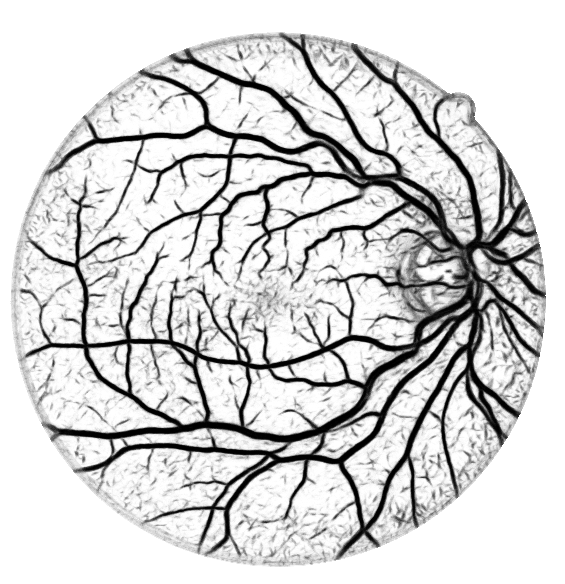
\includegraphics[width=0.3\columnwidth]{\figpath/retina/02_segmentation_gabor_inv.png} &
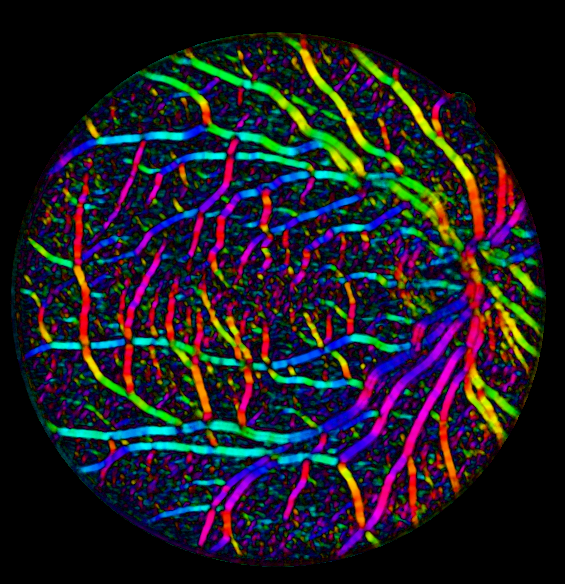
\includegraphics[width=0.3\columnwidth]{\figpath/retina/02_orientation_mag} \\
%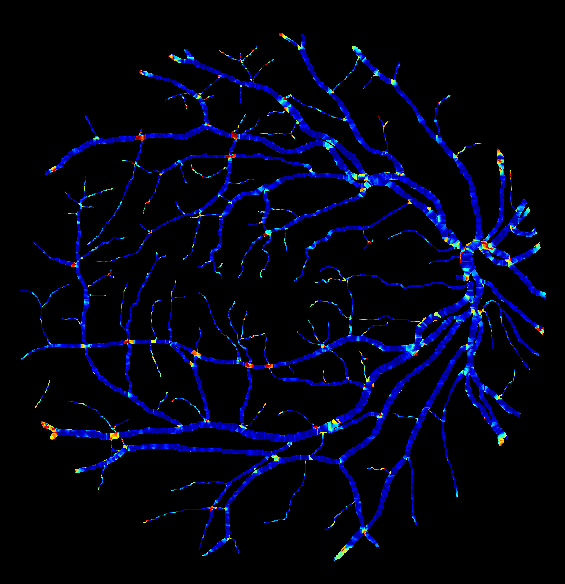
\includegraphics[height=0.15\textheight]{\figpath/retina/002_abs_error} \\
(a) & (b) & (c) \\
\noalign{\smallskip}
\end{tabular}
%
\caption{Estimating orientation in retinography: %
(a) input image; %
(b) segmentation of vessels by random forest classification of Gabor features; %
(c) orientation (indicated by colour) estimated using random regression over Gabor~features.}
\label{f:first_pic}
\end{figure}

% Specific aims of the study
Given an image, our aim is to determine where any linear structures exist in the image, and to measure values that correspond to low-level properties such as orientation, width, and cross-sectional profile. Although these properties form the basis of higher level, application-specific analysis (classifying structure as \emph{road}, \emph{rail} or \emph{river} in aerial photographs, for example), our focus is purely on computing the local attributes as accurately and robustly as possible; by improving the accuracy of the values we estimate, it follows logically that performance should improve for all higher level analysis methods that use these values as inputs.\footnote{Any algorithm that does not benefit from better input should be regarded with suspicion.}

%For example, any method to move from a map of vessel probabilities and predicted orientations in a retinograms, to an explicit grouping of pixels that belong to individual vessels, is likely to benefit from a priori knowledge of the spatial arrangement vessels in that image class and the physical model of how vessels grow and bifurcate. Such a method will therefore be very different from that needed to group a similar set of local information into the road, rivers etc present in an image for aerial analysis

With this focus, we have two objectives: extract, at every image location, structural information that is rich enough to capture the underlying image properties yet sparse enough to be computed efficiently; and combine this raw local information to predict output values of interest (such as orientation).


% Review other people's attempts at solving the problem, and why they are found wanting
\subsection{Related Work}
\comment{
There is no 3D analogue of the \dtcwt{}. Therefore, we should avoid 3D datasets and related work as much as possible - this paper is solely about the analysis of 2D image structures. This includes aerial photography, retinal images, fingerprints and palmprints, surface inspection, and possibly fibre analysis.
}

Because previous attempts at detecting and measuring curvilinear structures have been surveyed elsewhere, from the general~\cite{Papari_Petkov_IVC11} to the application-specific~\cite{Kirbas_Quek_ACMCS04,Lesage_etal_MIA09}, here we briefly review only a few papers in applications areas of specific interest. We will also discount the very basic detection methods that simply threshold an image~\cite{Jiang_Mojon_TPAMI03} and very complex methods that use techniques such as phase fields~\cite{Peng_etal_IJCV09}, leaving us free to focus on the most popular approaches that apply a bank of filters to the image before interpreting the responses in a way that accentuates the `lineness' at every pixel.

Early examples modelled a curvilinear structure as an image `ridge', typically defined using second order derivatives and formulated either as a Hessian problem~\cite{Frangi_etal_MICCAI98,Sato_etal_MIA98} or as responses to a derivative filter~\cite{Staal_etal_TMI04,Aylward_Bullitt_TMI02,Steger_TPAMI98,Koenderink_vanDoorn_TPAMI92}. Interpreting the responses to these filters used hand-crafted equations based on the differential geometry of the image `surface'~\cite{Frangi_etal_MICCAI98,Sato_etal_MIA98}.

With the maturing of machine learning, it was recognized that hand-crafting could be replaced by flexible statistical models whose parameters were optimized to agree with input-output training example pairs; Gaussian mixture models~\cite{Soares_etal_TMI06}, %
artificial neural networks~\cite{Marin_etal_TMI11,Minh_Hinton_ECCV10}, %
support vector machines~\cite{Ricci_Perfetti_TMI07,Gonzalez_etal_CVPR09}, and %
$k$-nearest neighbour classifiers~\cite{Staal_etal_TMI04} were all popular choices. Not only are these methods well-established and understood within machine learning, but a learnt statistical model can also accommodate different sensing modalities (with different noise properties) and other `stuff' that is hard to hand-craft, making the resulting algorithms more easily transferrable.

In addition, learnt statistical models can be applied to \emph{any} vector of image features to predict the quantity of interest, and are not tied to a particular feature type with specific theoretical properties. Furthermore, flexible statistical models permit the option to include hand-crafted, application-specific features where beneficial~\cite{Staal_etal_TMI04}. As a result, subsequent studies were free to use alternative filter banks and features based on %
matched filters or templates~\cite{Chaudhuri_etal_TMI89,Pechaud_etal_CVPR09,Dixon_Taylor_IPC79,Hoover_etal_TMI00,Ricci_Perfetti_TMI07}; %
derivatives of a first~\cite{Cai_Chung_MICCAI06} or higher than second~\cite{Gonzalez_etal_CVPR09} order; %
Gabor filters~\cite{Soares_etal_TMI06,Dabbah_etal_MIA11}; %
moments~\cite{Marin_etal_TMI11}; %
principal component analysis~\cite{Minh_Hinton_ECCV10}; %
wavelet transforms; %
and the monogenic signal. %
Some of these filter banks have been evaluated previously in a brief comparison~\cite{Ayres_Rangayyan_JEI07}, though the authors admit that not all filters were compared exactly on a like-for-like basis; our work builds on this comparison.

As well as permitting flexibility in the choice of input feature vector, learnt statistical predictors can be used to predict more than just the presence of a line. In recent studies, for example, orientation~\cite{Zwiggelaar_etal_TMI04,Ayres_Rangayyan_JEI07}, width~\cite{Steger_TPAMI98,Zwiggelaar_etal_TMI04} and multi-class labels~\cite{Zwiggelaar_etal_TMI04} have all been predicted from image feature vectors.

Other facets of tube detection and measurement are interesting though not directly relevant to this work: %
detecting lines at multiple scales~\cite{Lindeberg_IJCV98,Sato_etal_MIA98}; %
dealing with junctions and bifurcations where multiple lines meet at a point~\cite{Chen_etal_TPAMI00};
regularizing estimated lines via snakes~\cite{Laptev_etal_MVA00} or dynamic programming~\cite{Gruen}; %
and line following or tracking~\cite{Aylward_Bullitt_TMI02,Perez_etal_ICCV01}.

% Describe what we do, and why it is better than preceding works
\subsection{Our Contributions}
% Briefly outline our attempt at solving the problem, and why it should be better than the solutions that have preceded it
This paper presents three contributions that advance the current body of knowledge in the analysis of curvilinear image structures.

First, we provide a detailed comparison of commonly used image filter banks in the context of their suitability for extracting the local image information pertaining to curvilinear structure. In doing so, we describe the desirable properties of a suitable filter bank, therefore enabling us to make a principled choice that balances the richness of the extracted information against efficiency (both computational and storage). This analysis leads us to apply a previously unexploited image filter -- the dual-tree complex wavelet transform (\dtcwt{}) -- to the task of curvilinear feature analysis. The \dtcwt{} benefits from specific properties, such as efficiency and phase information, that address the shortcomings of existing popular image filters (\sref{s:filtering}).

Second, we investigate supervised learning approaches that, after training on a set of (input feature vector, target label) example pairs, turn a previously unseen feature vector of filter responses at a given location into an estimated output value. Specifically, we include the Random Forest statistical method to predict outputs, and compare this to techniques that have been previously used. For line detection (\ie~image segmentation), we show that a carefully selected filter bank, coupled with a modern learning method that is capable of dealing with non-linear data, produces results that match or exceed the state-of-the-art without relying on application-specific assumptions to boost performance. For orientation, we show how to formulate the learning problem such that angle wraparound is dealt with correctly, and in doing so produce\comment{ significantly} better estimates than existing methods that compute orientation analytically. In addition, we show how predicting output responses via machine learning allows us to estimate the error associated with the predictions, which we propose may in itself be of use in further processing.

Third, we explore the similarities and differences between these different approaches, and present empirical evidence of which work best in practice for real images including retinography and corneal confocal microscopy.

In all cases, we back up theoretical claims for filter performance with thorough experimental validation on both synthetic and real data.

%Finally, if for a given image class we know of additional properties that will be useful to predict and that can be reliably labelled on our training data (for example, a further classification of structure in aerial images to roads and rivers) these can easily be added to our protocol.

%\clearpage

\section{Target Output Labels}
Our approach to analyzing and understanding images containing linear structure is to use statistical learning methods to recognize patterns present in training data in order to predict useful information in previously unseen images. More specifically, we focus on two tasks: detecting linear structures in the image; and measuring the orientation of linear structures. Though the input image features are common across both tasks, the output label we wish to predict is task-dependent.

\subsection{Detecting Linear Structure}

One of the most basic tasks in image interpretation is to determine which pixels correspond to linear structures such as vessels, spicules and road, and which pixels correspond to background data in which we have no interest. Throughout we refer to the former as CLS pixels, and the latter as background pixels.

\comment{Segmenting curvilinear structures such as blood vessels, ducts and nerve fibres in medical images is an important task, as shown by the extensive literature in the field~\cite{Papari_Petkov_IVC11,Staal_etal_TMI04,Ricci_Perfetti_TMI07}.}

In our definition of CLS, each structure has a finite width and can be unambiguously differentiated from the image background (regardless of what other structures may be present in the background). As such, for a given class of images (retinograms, aerial maps etc), it is possible to obtain training images in which each pixel can either be labelled as belonging to a CLS or belonging to background. By convention, we assign the former a class label $\mathcal{C}=1$ and the latter $\mathcal{C}=0$. Typically these labels are based on a ground truth segmentation that has been generated by an expert human observer

To segment an unseen image, we train a statistical classifier to predict an output label $C_{est}(p) \in [0, 1]$ at each pixel $p$, such that $C_{est}(p)$ represents the probability that $p$ belongs to a CLS.

%\subsection{Classifying Linear Structure}
%\label{s:review_orientation}
%
At a low and intermediate level, knowing the orientation of curvilinear linear structure is important for steering computation~\cite{Sonka_99}, extracting profiles~\cite{Zwiggelaar_etal_TMI04,Staal_etal_TMI04}, grouping and tracking curvilinear features~\cite{Aylward_Bullitt_TMI02}, and directional filtering such as nonmaximal suppression and anisotropic diffusion~\cite{Perona_PAMI90}. 
%Estimating the local \emph{orientation} of curvilinear structure is also important, though the literature in this area is more limited~\cite{Freeman_Adelson_TPAMI91,Koenderink_vanDoorn_TPAMI92}.
Applications at a high level, however, are more diverse.

As well as knowing where the linear structures are, we may also wish to know where they are heading.%
%The literature on classifying curvilinear structures in mammograms is limited. We are aware of one study that demonstrated the feasibility of distinguishing between different types of structure using cross-sectional profiles obtained from manually annotated curvilinear structures, but did not obtain very satisfactory results when the method was fully automated~\cite{Zwiggelaar_etal_TMI04}. We recently reported preliminary classification (but not detection) results using our current approach~\cite{Chen_etal_IWDM10}.

In mammography, however, we concentrated on the task of distinguishing between spicules (that are an indicator of malignancy) and other curvilinear structures, such as ducts, that are of little consequence.
%
%% Define the output labels in a classification (i.e. multi-class classification) task
%
When using a statistical classifier to discriminate between $k>2$ classes, the target label we assign to examples from the $i$th class is $k$-vector whose $i$th element is $1$, and all other elements are $0$.%

\subsection{Measuring Orientation}
\label{s:measuring_orientation}
At a low and intermediate level, knowing the orientation of CLS is important for steering computation~\cite{Sonka_99}, extracting profiles~\cite{Zwiggelaar_etal_TMI04,Staal_etal_TMI04}, grouping and tracking curvilinear features~\cite{Aylward_Bullitt_TMI02}, and directional filtering such as nonmaximal suppression and anisotropic diffusion~\cite{Perona_PAMI90}. Applications at a high level, however, are more diverse. *This feels unfinished?*

CLS orientation may be computed by assuming that it can be expressed as a (typically nonlinear) function of the responses to a given set of filters. Theoretically, we know this to be true for some filter banks (\eg~second derivatives of a Gaussian), though there are some complications.

First, when filters are applied at more than one scale we must ensure that we use the responses from the best scale for the true line width; analytic methods~\cite{Karssemeijer_teBrake_TMI96,Mei_etal_IVC09} assume this is the scale with the greatest response, though this is not guaranteed in the presence of noise. Second, any analytic method that assumes noise to be additive and Gaussian may suffer when this is not the case; this is a particularly a risk in medical applications (\eg~ultrasound has multiplicative Rayleigh noise). Third, for some filter banks (such as the \dtcwt{}) an analytic solution is not well defined.

Our solution to these problems is to apply statistical methods that learn the association between input filter responses and an output orientation label over a set of training data. Given a ground truth segmentation, we can thin the CLS to a binary skeleton, again using the fact CLS are defined to have finite width. We can then compute the local orientation of each skeletonised CLS pixel, and subsequently label any CLS pixel $p$, with the orientation of the nearest skeletonised pixel. Throughout we refer to this ground truth orientation as $\theta_{gt}(p)$.

Note that where CLS branch or intersect, this orientation is ill-defined. For now, we omit such pixels from the training data. However, we discuss later how this problem may be overcome, and indeed how orientation predictions could actively be used to help detect these features in future work.

\label{s:orientation_representation}
%
Because orientation is a continuous variable, it is appropriate to estimate its value by regression. Orientation, however, violates a common assumption in that it does not live in a Euclidean space; adding $2\pi$ radians gives the same orientation, for example. Also, orientation (unlike \emph{direction}) is only defined over half the circle; orientations exactly $\pi$ radians apart are also considered to be identical.

A different representation is therefore needed, and one that respects these two conditions uses a unit vector in the complex plane where the underlying angle is doubled such that two orientations exactly $\pi$ radians apart are mapped to the same complex value~\cite{Mardia_Jupp_00}:

\begin{equation}
	t_{gt}(p) = \cos 2\theta_{gt}(p) + i\sin 2\theta_{gt}(p)
\end{equation}

% Difference between two orientations
Representing orientation as a complex vector also allows us to define a distance measure between two values -- an estimated value, $t_{est}$, and ground truth, $t_{gt}$, for example:

\begin{equation}
	2\theta_{err}(p) = |\angle(t_{gt}(p) \cdot t_{est}^*(p))|,
\end{equation}
%
\noindent where $t^*$ denotes the complex conjugate of $t$. This error metric therefore accounts for the circular nature of orientation in a principled way.

% Interpreting the mean vector and its magnitude
Taking the mean over a set of orientations gives a complex vector whose angle is twice the average orientation over the set, and whose magnitude,
%
\begin{equation}
D = \left| \frac{\sum{t_k}}{N} \right|,
\label{e:angular_dispersion}
\end{equation}
%
\noindent defines the spread -- known as the \emph{angular dispersion} -- of the samples in the set~\cite{Mardia_Jupp_00}. By definition, $D$ reaches a maximum of $1$ when all $t_k$ are equal, and a minimum of $0$ when orientations are distributed uniformly about the circle or when the sample consists of pairs exactly $\pi$ radians apart.

\subsection{CLS width}
\label{s:output_width}
When the ground truth is skeletonised to compute target orientation labels, we can also apply a distance transform to label the width of each CLS pixel, which we refer to as $w_{gt}(p)$. If desired, $w_{gt}(p)$ is straightforward to regress directly -- in which case it may be preferable to label only the skeletonised (\ie centreline) pixels as CLS in the detection task. In unseen images, predictions of CLS centrelines may then be thinned, and a combination of predicted orientation and width used to estimate a complete segmentation of CLS.

However, we do not use that approach in this work, although $w_{gt}(p)$ is used during the evaluation of detection and orientation prediction to asses how performance varies a function of CLS width.

*width estimation results can be included results for these if we think it adds to the paper?*
%\clearpage

\section{Input Image Features}
\subsection{Filtering}
\label{s:filtering}

Having defined target outputs that we intend to predict, in this section we describe what input features we will base our learning on. Our basic approach is to convolve an image with a bank of filters, generating a set of responses at each pixel that represent local image structure.

To complete the two tasks defined in the previous section, this requires that the set of responses for any given CLS pixel should be distinguishable from the responses of any background pixel; and the filters should be directionally selective to predict orientation. Whilst this may seem trivial to state, we note that the former condition is often not satisfied by many of the filter banks previously used to detect CLS.

We now describe each of the filter banks tested in this paper.

\begin{figure}[t]
\centering
\begin{tabular}{@{}c c c c@{}} % @{} removes padding around the edge of the table
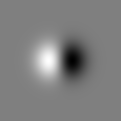
\includegraphics[width=0.2\columnwidth]{figs/filtering/Gx} &

\includegraphics[width=0.2\columnwidth]{figs/filtering/Gxx} &
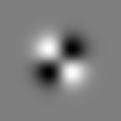
\includegraphics[width=0.2\columnwidth]{figs/filtering/Gxy} &

\includegraphics[width=0.2\columnwidth]{figs/filtering/Gxx-Gyy} \\
(a) & (b) & (c) & (d) \\
\noalign{\smallskip}
%
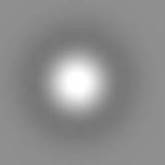
\includegraphics[width=0.2\columnwidth]{figs/filtering/mono_b} &
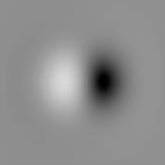
\includegraphics[width=0.2\columnwidth]{figs/filtering/mono_hx} &
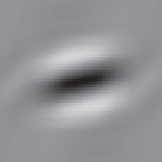
\includegraphics[width=0.2\columnwidth]{figs/filtering/dt_cwt_r4} &
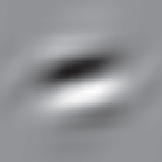
\includegraphics[width=0.2\columnwidth]{figs/filtering/dt_cwt_c4} \\
(e) & (f) & (g) & (h) \\
\noalign{\smallskip}
\end{tabular}
%
\caption{(a)~First derivatives $\Gx = \Gy^T$; (b-d)~Second derivatives, $\Gxx = \Gyy^T$, $\Gxy$; and $\Gxx-\Gyy$; (e,f)~Monogenic signal filters $B$ and $h_x = h_y^T$; (g,h)~Real and complex responses of the \dtcwt~ $15^\circ$ subband.}
\label{f:filters}
\end{figure}

\subsubsection{Gaussian derivatives}
\label{s:filtering_secondderivs}
%
Derivatives of a Gaussian kernel are probably the most commonly used set of filters for linear structure detection (certainly within the context of vessel segmentation in medical images). Throughout, we use $G \equiv G(x,y|\sigma)$ to refer to a 2-dimensional Gaussian kernel with standard deviation $\sigma$, and use subscripts to denote derivatives of $G$ with respect to a particular direction.

The first derivatives of a Gaussian kernel, taken separately with respect to the horizontal ($G_x$) and vertical ($G_y$) axes, are odd filters (\ie $G_x(-x,y) = -G_x(x,y)$ and $G_y(x,-y)=-G_y(x,y)$) that can be used to estimate the strength and direction of the image gradient at each pixel. As such, they are commonly used to detect asymmetric image features (\ie edges) that are associated with a large image gradient in the direction perpendicular to the edge's orientation.

However, a basic property of CLS is that they have approximately symmetric profile and so the first derivative responses of a pixel at the centre of a CLS will be near zero.

Accordingly, when CLS are the structures of interest, it is typical to use second derivatives. Deriving $G_x$ and $G_y$ again both horizontally and vertically, produces three filters, $\Gxx$, $\Gyy$ and $\Gxy = \Gyx$, that can be combined to generate a filter
%
\begin{equation}
G_\theta = \Gxx \cos^2(\theta) + \Gyy \sin^2(\theta) + \Gxy \sin(2\theta)
\label{e:secondderivs_filter}
\end{equation}
%
with even symmetry that resembles a bar or ridge feature at any arbitrary direction $\theta$. However, we need never actually compute $G_\theta$ and apply it to an image, as its response $I_{G_{\theta}}$ may be computed directly from the responses to the separable filters, $\Ixx$, $\Iyy$ and $\Ixy$
%
\begin{equation}
I_{G_\theta} = \Ixx \cos^2(\theta) + \Iyy \sin^2(\theta) + \Ixy \sin(2\theta)
\label{e:secondderivs_response}
\end{equation}

This response function has four stationary points in the range $[0,2\pi)$, occurring at
%
\begin{equation}
\theta = \frac{1}{2} \tan^{-1}\left( \frac{2\Ixy}{\Ixx-\Iyy} \right).
\label{e:secondderivs_orientation}
\end{equation}
%
\noindent Two of these points, $\hat{\theta}$ and $\hat{\theta}+\pi$, correspond to the directions in which the filter is aligned with the feature and the \emph{absolute} value of the response is maximal; the other two points correspond to the two perpendicular directions ($\hat{\theta}^\perp$ and $\hat{\theta}^\perp+\pi$).

Because, however, the maximal absolute response may correspond to either a maximum or minimum (depending on whether the underlying feature is light-on-dark or vice versa) the only way to find out which of the two perpendicular directions has maximal absolute value is to evaluate the response at both and choose the direction corresponding to the larger absolute value. As a result, estimating orientation from second-order derivatives becomes a nonlinear problem.

*Efficient approximations to computing second-order derivatives of the Gaussian can be achieved through Haar-like approximations to the derivative filters~\cite{Bay_etal_CVIU08} or by approximating the Gaussian filter and applying local finite differences~\cite{Kovesi_DICTA10} *could omit?*.

*Note this approach is often reformulated by creating a Hessian matrix \cite{} with the $xx$ and $yy$ derivatives on the lead diagonal and the $xy$ derivatives on the opposing diagonal. Solving this matrix produces eigen vectors with direction $\hat{\theta}$ and $\hat{\theta}^\perp$ and magnitude $I_{\hat{\theta}}$ and $I_{\hat{\theta}^\perp}$ *include as footnote/*.

Second derivatives are used on the assumption that when steered to match the orientation of a CLS, the response will be large, whilst the response in the perpendicular direction will be near-zero. Thus CLS can be distinguished from flat backgrounds (both responses near-zero) or circular blob-like structures (both responses large). Moreover \eref{e:secondderivs_orientation} provides an elegant solution for determining this orientation analytically -- although as noted previously, and justified experimentally in \sref{s:experiments_1}, we prefer a learning based approach to predicting orientation from the filter responses.

However, in either an analytical or learning approach, there are two problems in using second derivatives alone. Firstly, a strong edge in the image will produce an "echo" response that cannot be distinguished from the response at the centre of a CLS. This may seem an arbitrary construct; however it is easy find examples in real data. For example, the edge of the optic disc in a retinogram (\fref{f:drive_odd_even}) is often misclassified as a vessel, whilst similar artifacts may occur at the edges of lesions or near the pectoral muscle in mammograms.

\begin{figure}[t]
\centering
\begin{tabular}{@{}c c c@{}}
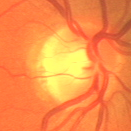
\includegraphics[width=0.3\columnwidth]{\figpath/retina/02_optic} &
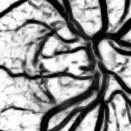
\includegraphics[width=0.3\columnwidth]{\figpath/retina/02_optic_g2d_inv} &
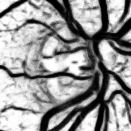
\includegraphics[width=0.3\columnwidth]{\figpath/retina/02_optic_g12d_inv} \\
%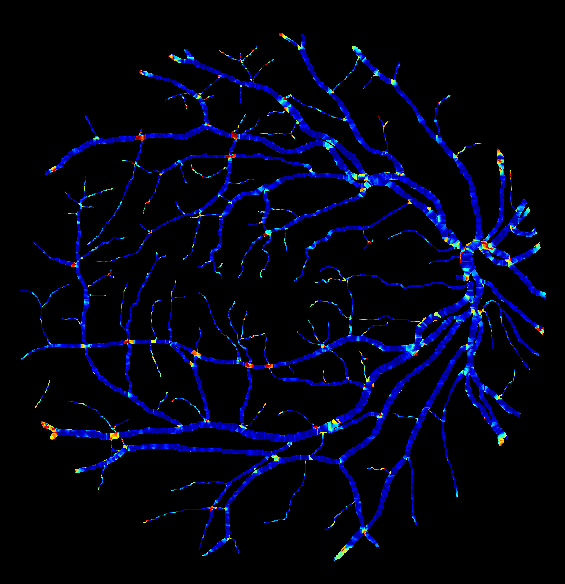
\includegraphics[height=0.15\textheight]{\figpath/retina/002_abs_error} \\
(a) & (b) & (c) \\
\noalign{\smallskip}
\end{tabular}
%
\caption{Detecting vessels in retinography: %
(a) Magnified region containing optic disk; %
(b) Segmentation using only even filter responses as features: the false positive predictions
at the edge of the disk have similar strength to neighbouring vessels; %
(c) Segmentation using odd and even filter responses: false positives are still present, but at a
much lower strength to nearby vessels;
}
\label{f:drive_odd_even}
\end{figure}

Secondly, due to noise in the image, the symmetric profile of a CLS may be disrupted to the extent that not only does equation \eref{e:secondderivs_orientation} produce inaccurate estimations of orientation, the responses themselves hold no usual information for a machine learning algorithm to take advantage of. Again, this can be seen clearly in real data, particularly in structures that have a width of only one or two pixels, such as the smallest vessels in retinograms.

The first problem tells us that it is not enough to have only filters designed to match the shape profile of CLS if the filters responses cannot distinguish other structures in the image background. The second problem says that we cannot rely on the assumptions we make about CLS in real images corrupted by noise.

Combining both ideas motivates us to use a filter bank that more generally represents \emph{any} image feature, rather than one particular structure type. Our goal then is not to make a priori assumptions about the filters responses, but simply to ensure the set of filter responses at a pixel of any one structure type is different from those of a pixel belonging to any other structure. It is then up to our chosen machine learning algorithm to match the various patterns of responses present in the training data to the output measure of interest.

An intuitive solution is to supplement the \emph{even} second derivative filters with the \emph{odd} first derivatives. However, we prefer the approach recommended in \cite{Freeman_Adelson_TPAMI91}, using the Hilbert transform of the second derivatives to provide filters with odd symmetry. In this method, four separable basis filters
%
\begin{equation}
H_a = 0.9780(2.2540x + x^3)G
\label{e:secondderivs_hilberta}
\end{equation}
\begin{equation}
H_b = 0.9780(0.7515 + x^2)yG
\label{e:secondderivs_hilbertb}
\end{equation}
\begin{equation}
H_c = 0.9780(0.7515 + y^2)xG
\label{e:secondderivs_hilbertc}
\end{equation}
\begin{equation}
H_d = 0.9780(2.2540y + y^3)G
\label{e:secondderivs_hilbertd}
\end{equation}
%
may be used to generate a steered response
\begin{align}
   I_{H_\theta} =
     &I_{H_a} \cos^3(\theta) \nonumber \\
   - &I_{H_b} 3\cos^2(\theta)\sin(\theta) \nonumber \\
   + &I_{H_c} 3\cos(\theta)\sin^2(\theta) \nonumber \\
   - &I_{H_d} \sin^3(\theta)
\label{e:secondderivs_hilberts}
\end{align}

The advantage of using $I_{H_\theta}$ (as opposed to a first derivative response) is that it may be combined with $I_{G_\theta}$ to generate magnitude and phase
%
\begin{equation}
M_\theta = \sqrt{I_{G_\theta} + I_{H_\theta}}
\label{e:secondderivs_mag}
\end{equation}
%
%
\begin{equation}
\psi_\theta = \tan^{-1}\left( \frac{I_{G_\theta}}{I_{H_\theta}} \right)
\label{e:secondderivs_phase}
\end{equation}
%
These have an intuitive interpretation where the value of $M_\theta$ at any pixel tells us whether a structure with orientation $\theta$ is present, whilst $\psi_\theta$ tells us the structure's profile (in the direction $\theta^{\perp}$), as it varies from a valley ($\psi_\theta=\nicefrac{\pi}{2}$), to a step ($\psi_\theta=0,\pi$), to a ridge ($\psi_\theta=\nicefrac{\pi}{2}$).

This gives us three basic forms of Gaussian responses to use as features:
\begin{enumerate}
  \item The raw responses to the separable filters at each scale:
  \begin{equation*}
    \{I_{G_xx}, I_{G_xy}, I_{G_yy}, I_{H_a}, I_{H_b}, I_{H_c}, I_{H_d}\}
  \end{equation*}

  \item Steered responses at a number of discrete angles (typically $N_\theta=6$), spread evenly around the circle:
  \begin{equation*}
    \{I_{G_\theta}, I_{H_\theta}\}, \; \theta = [ \nicefrac{i\pi}{N_\theta} ]
  \end{equation*}
  \item Steered responses, converted to magnitude and phase:
  \begin{equation*}
    \{M_\theta, \psi_\theta\}, \; \theta = [ \nicefrac{i\pi}{N_\theta} ]
  \end{equation*}
\end{enumerate}

To account for CLS with different widths, the separable filters are applied at multiple scales, typically by varying $\sigma$ in octave scales (\ie increasing powers of two), and the resulting responses (converted into one of the three forms above) concatenated into a single feature vector. Alternatively, responses at different scales may be generated by successively downsampling the image by a factor of two (\ie decimating) and then applying a filter with fixed $\sigma$. The decimated responses must then be interpolated to the resolution of the original pixel grid to produce and equivalent feature vector.

The latter approach will be much faster to compute, but the interpolated responses at coarser scales may be less robust (\ie more susceptible to noise) than those computed from the full-size image. We test both approaches in \sref{s:experiments_2}.


\subsubsection{Gabor filters}
\label{s:filtering_gabor}
A Gabor filter pair consists of one sine and one cosine function, in two dimensions, windowed with a Gaussian kernel:

\begin{equation}
W_{re}(x,y;\lambda,\theta,\sigma,\gamma) = \exp \left( -\frac{u^2 + \gamma^2 v^2}{2\sigma^2} \right)
    \cos \left( \frac{2\pi u}{\lambda} \right)
\label{e:gabor_real}
\end{equation}
\begin{equation}
W_{im}(x,y;\lambda,\theta,\sigma,\gamma) = \exp \left( -\frac{u^2 + \gamma^2 v^2}{2\sigma^2} \right)
    \sin \left(  \frac{2\pi v}{\lambda} \right)
\label{e:gabor_imag}
\end{equation}
where
\begin{align}
u = x\cos\theta + y\sin\theta \\
%
v = -x\sin\theta + y\cos\theta
\label{e:gabor_xy}
\end{align}
%
Thus $\sigma$ again controls the filter's scale, $\gamma$ varies the shape of the Gaussian kernel (we always use a circular kernel with $\gamma=1$ although in other work elliptical kernels have been used \cite{Dabbah_etal_MICCAI10}), and $\lambda$ controls the frequency of sine waves. Here, we adopt the usual approach of fixing the ratio between $\sigma$ and $\gamma$ at each scale.

Because the even $W_{re}$ and odd $W_{im}$ filters are Hilbert pairs (\ie the differ in phase by $90\deg$), at each scale and orientation we can use their responses $I_{re}$ and $I_{im}$ directly as features, or combine them into a magnitude and phase. Similarly, we have the same choice of filtering at multiple scales by varying $\sigma$, or downsampling the image and interpolating the decimated responses.

Because Gabor filters are directionally sensitive, and can also recover phase information, they are a popular choice of filter in image processing applications~\cite{Daugman_TASSP88}. However, like Gaussian derivatives, where they have also been used to detect CLS, it is often only the even filter $W_{re}$ that is used. For the same reason we match $G_\theta$ with $H_\theta$, we recommend using both $W_{re}$ and $W_{im}$, and show experimentally the advantages of doing so in \sref{s:experiments_2}.

An advantage of Gabor filters, is that by varying the ratio of $\lambda$ to $\sigma$, they allow us to control the directional selectivity of each oriented sub-band in a manner not available to Gaussian derivatives. \fref{f:oriented_responses}a shows the magnitude of $I_{G_\theta}$ and $I_{H_\theta}$ for a pixel on a simple line feature rotated through $180\deg$; the responses have been steered to generate six equally spaced sub-band about the circle. \fref{f:oriented_responses}b shows the responses to six equivalently oriented Gabor filters - note how the drop-off from maximum to minimum response is much faster for each Gabor sub-band. This suggests Gabor filters may be better suited to separating CLS by angle, and thus predicting orientation.

However, unlike Gaussian derivatives, Gabor filters are neither separable nor steerable, although methods to approximate steerability have been explored~\cite{Teo_1987,Perona_PAMI95}. Therefore, they must be applied exhaustively over a discrete set of orientations at each scale. This makes them much more computationally expensive, and also requires more memory (if all responses are to be stored simultaneously).

In an attempt to get the best of both worlds, we next consider a filtering scheme, that offers similar directional selectivity to Gabor filters, at a fraction of the computational cost, and has so far been unexploited in applications analysing CLS *what about our own work?*.

\begin{figure}[t]
\centering
\begin{tabular}{@{}c c c@{}} % @{} removes padding around the edge of the table
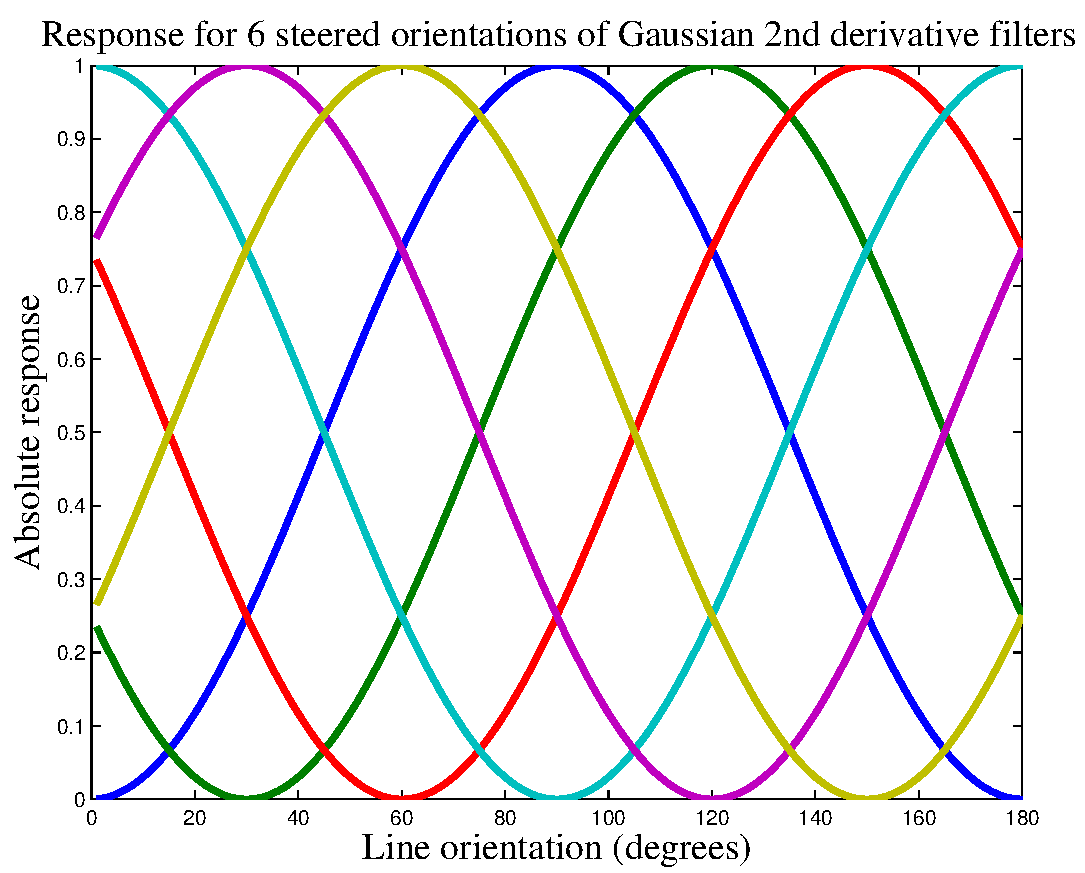
\includegraphics[width=0.3\columnwidth]{figs/filtering/g2d_oriented_response} &
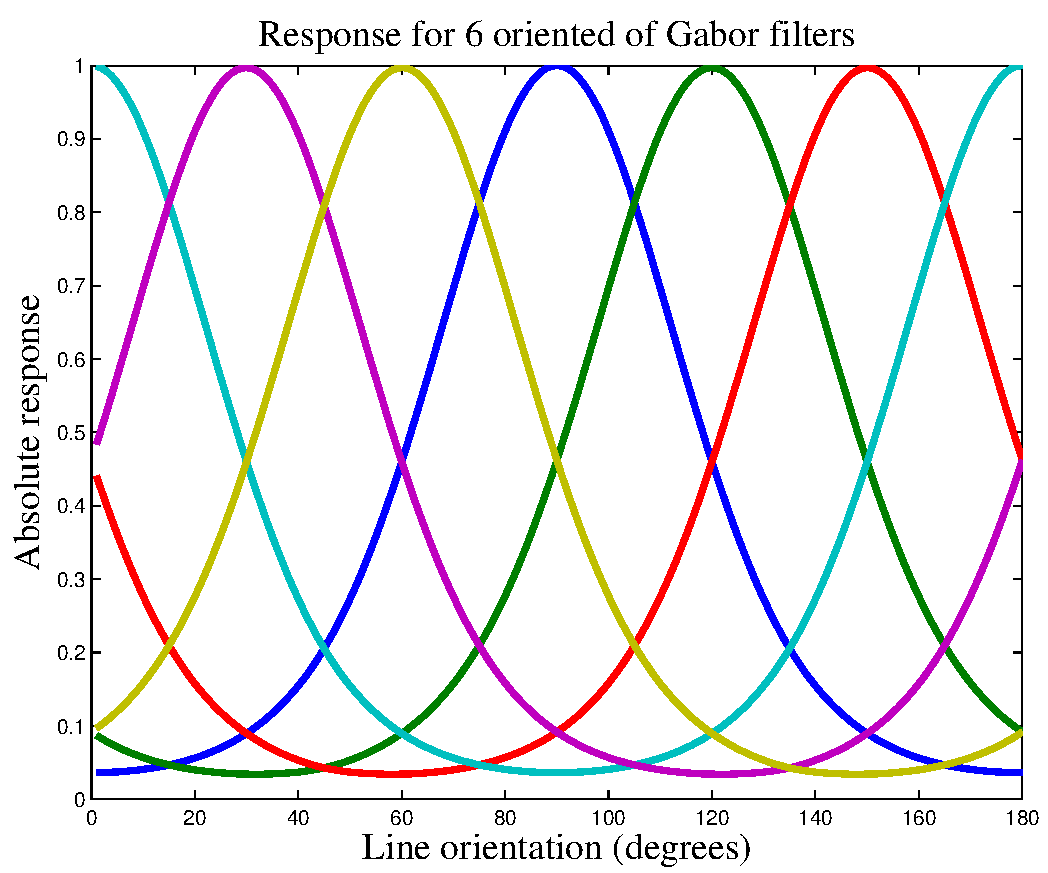
\includegraphics[width=0.3\columnwidth]{figs/filtering/gabor_oriented_response} &
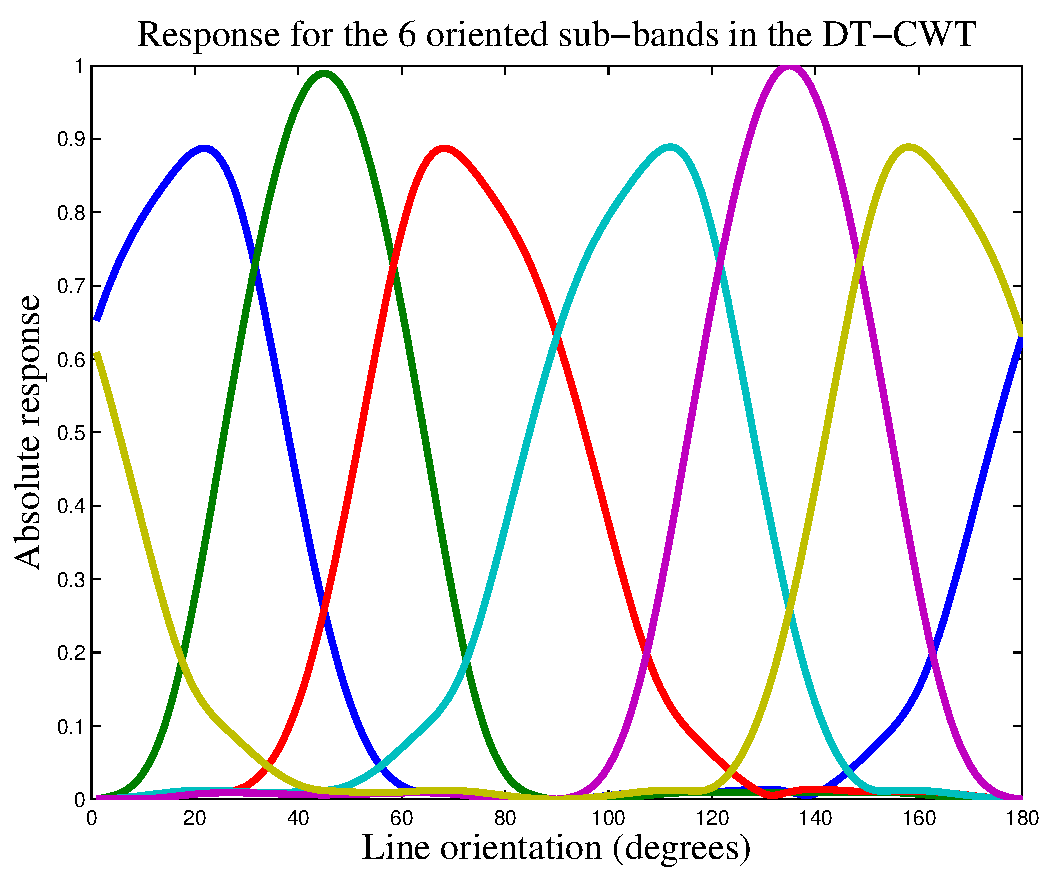
\includegraphics[width=0.3\columnwidth]{figs/filtering/dt_oriented_response} \\
(a) & (b) & (c) \\
\noalign{\smallskip}
\end{tabular}
%
\caption{Oriented sub-band response as a function of CLS orientation (a) Gaussian; (b)Gabor; (c)\dtcwt{} }
\label{f:oriented_responses}
\end{figure}


\subsubsection{The Dual-tree Complex Wavelet Transform}
\label{s:filtering_dtcwt}

The Dual-Tree Complex Wavelet Transform (\dtcwt{}~\cite{Kingsbury_ACHA01}) was developed to overcome the problems inherent in discrete wavelet transforms - their lack of directional selectivity and shift-invariance - whilst remaining fully invertible and maintaining the efficiency of decimation.

Considered as a filtering scheme, the \dtcwt{} combines separable high and low-pass filters to produce sub-bands at six orientations at each scale: $\pm 15\deg$, $\pm 45\deg$ and $\pm 75\deg$. Each sub-band contains complex coefficients, the real and imaginary parts of which are equivalent to the responses from a pair of filters that differ in phase by $90\deg$~(\fref{f:filters_dtcwt}) -- although neither filter has perfect odd or even symmetry.

As recommended in~\cite{Kingsbury_ECSP06}, we use the Q-Shift filters, and include the additional filters designed to reduce the wave frequencies of the $\pm 45\deg$ sub-bands so that they lie closer to those at $\pm 15\deg$ and $\pm 75\deg$, as well as adjusting all six sub-bands that the phase at the centre of the impulse response of each wavelet is zero.

% Multiresolution filtering
To compute filter responses at different scales, the image is repeatedly downsampled by a factor of two in every axis before applying the same separable filter pairs again. This makes the \dtcwt{} extremely fast to compute. Moreover, downsampling means the representation has a redundancy of just 4:1, making it feasible to store the decomposition of even large images (by contrast a full Gabor representation, computed at six orientations over 5 scales has a redundancy of 60:1).

To get the response for every scale at a given location on the original pixel grid, the decimated filter responses are interpolated using the method defined in~\cite{Anderson_etal_ICIP05}. Because the transformation is designed to be shift-invariant, these interpolations are well-defined and theoretically valid.

As with Gabor and Gaussian responses, at each scale and orientation we can choose to use either the raw responses (\ie the real and imaginary parts of the interpolated complex coefficients) directly as features or convert the pair of responses into magnitude and phase.

The response of each sub-band to a line rotated about the circle is shown in \fref{f:oriented_responses}c -- note how the sub-bands have a similar directional selectivity to the Gabor filters (\fref{f:oriented_responses}a). However, unlike the Gaussian and Gabor filters, the \dtcwt{} sub-bands do not have perfect rotation symmetry. The effect this has on features constructed from \dtcwt{} coefficients is explored in \sref{s:experiments_2}.


\subsubsection{The Monogenic Signal}
\label{s:filtering_monogenic}

*When you put forward the theoretical arguments - there really isn't much to call for the Monogenic Signal*
The final filtering scheme we include is also designed to efficiently compute magnitude, phase and orientation at multiple scales in an image. The Monogenic Signal~\cite{Felsberg_Sommer_TSP01} achieves using three filters: one even band-pass filter $B$, and an odd quadrature pair of filters $h_x(x,y) = x/f(x,y)$ and $h_y(x,y) = y/f(x,y)$ where $f(x,y) = 2\pi(x^2 + y^2)^{\frac{3}{2}}$ (\fref{f:filters_monogenic}). These filters are combined to compute a magnitude~($M$), phase~($\psi$) and orientation~($\theta$) at every location in the image:

\begin{align}
M       &= \sqrt{{I_B}^2 + {I_{hx}}^2 + {I_{hy}}^2}
\label{e:monogenic_amplitude} \\
%
\psi	  &= \tan^{-1}\left[ \frac{I_B}{\sqrt{{I_{hx}}^2 + {I_{hy}}^2}} \right]
\label{e:monogenic_phase} \\
%
\theta  &= \tan^{-1}\left[ \frac{I_{hy}}{I_{hx}} \right]
\label{e:monogenic_orientation}
\end{align}

Scale is controlled by the bandpass filter $B$, for which we use log-Gabor filter, defined in the frequency domain as

\begin{equation}
B(\omega) = \exp \left( -\frac{ \log(\nicefrac{r}{f_o})^2 } {2 \log(\sigma_o)^2} \right)
\label{e:monogenic_bandpass}
\end{equation}
%
where $f_o$ is the centre frequency of the filter, and $\sigma_o$ controls the bandwidth (we use $\sigma_o=0.65$, and double $f_o$ at each scale to obtain bands of approximately 1 octave).

The efficiency with which the Monogenic Signal computes local measures of magnitude, phase and orientation relative to a filter bank such as Gabor, has made it popular in several image processing tasks \cite{}, including an attempt to detect CLS in mammograms \cite{wai}.

However, whilst the Monogenic Signal combines both odd and even filters, the even filter $B$ is isotropic and therefore has no directional sensitivity. Consequently all orientation information comes from the odd filters $h_x$ and $h_y$, such that orientation cannot not be recovered for symmetric image features such as CLS (where both the numerator and denominator in \eref{e:monogenic_orientation} will be near zero).

\subsubsection{Other filter banks}

\label{s:filtering_extras}
Finally we acknowledge that there are of course many further filter banks we do not test in this paper, and for which an exhaustive comparison of results is unfeasible. However, we show \emph{how} and \emph{why} the properties of the filter banks we do test affect performance. Thus, given a set computational cost, we can make an informed choice of suitable filter bank for any given data.

We also show that a filter bank selected given these general criteria can produce features that outperform features handcrafted for a particular application.

One interesting concept we do not test is the idea of learning an optimal set of arbitrary filters for a given set of images, as in []. However, we believe that such an approach is only beneficial if the filters are optimised with respect to the task they need to perform (in our case and in [], separating the responses for CLS and background pixels within a classifier) and cannot see how optimising with respect to some other task (such as reconstructing the image in a maximally sparse way) is intrinsically a desirable thing to do. That said a comparison with the results in [] would be desirable if quantitative results on the DRIVE and STARE datasets were made available.

\subsection{Composing feature vectors from filter responses}
\label{s:composing_features}
Thus far we have described the four filter banks included in our experiments, and the basic form of features we can extract from each set of filter responses. Below we consider some additional modifications we can apply to these basic feature vectors.

\subsubsection{"Folding" phase}
\label{s:composing_features_complex}
When filter responses have been combined as phase $\psi$ and magnitude $M$, $\psi$ is computed using the four-quadrant arc-tangent, and is thus defined over $[-\pi, \pi)$. However, if an image is rotated through $180\deg$, the phase $\psi$ at any pixel becomes $\pi - \psi$ (\ie in polar form, it is reflected about the vertical axis). Thus if we define $\psi^*$ as

\begin{equation}
\psi^* =
\begin{cases}
      \psi          & \psi \in [\nicefrac{-\pi}{2}, \nicefrac{-\pi}{2}] \\
      \pi - \psi    & \psi \in [-\pi, \nicefrac{-\pi}{2}) \\
      \pi - \psi    & \psi \in (\nicefrac{\pi}{2}, \pi]
   \end{cases}
\label{e:folding_phase}
\end{equation}
%
then feature vectors using $M$ and $\psi$ ambivalent to $180\deg$ rotations. As we define orientation to be equivalent up to $180\deg$ rotations, this is a theoretically a desirable property.

\subsubsection{Rotation invariance}
\label{s:composing_features_rotation}
Given a set of responses at orientations spread evenly over the circle, a common approach is to rearrange the dimensions of the feature vector such that the orientation that produces maximum response occupies the same dimension in each feature vector, with the remaining orientations are permuted circularly so that the relative order is unchanged. The idea is to produce feature vectors with rotational invariance thus collapsing the size of the feature space (proportional to the number of discrete orientations in the filter bank) and making it easier for the classifier to do its job. With responses over multiple scales, we can choose either to allow the responses in each scale to shift independently or choose a single maximum orientation (\eg from the scale that produces maximum response) to use in all scales. Here we take the former approach although we have experimented with both and found little difference in performance.

\subsubsection{Pooling neighbourhood responses}
\label{s:composing_features_neighbours}
In addition to compiling responses across scale and orientation at each pixel, we can also pool the responses from neighbouring pixels. We have experimented with more exotic sampling schemes in which we interpolate responses in a circular pattern about each pixel, but have found that in practice simply sampling a $3\times3$ window of responses, with the labelled pixel in the centre of the window, provides most benefit. Of course this increases the dimension of the feature vectors nine-fold, but with machine learning algorithms (such as random forests) designed to cope with large dimensional features and plenty of training data (which is nearly always the case in this set up given each pixel in an image is a sample and thus even a small set of images typically contain millions of samples) this needn't be a problem.

\section{Statistical Learning Methods}
\label{s:learning_methods}
Having defined a label to assign to each pixel (either its class $\mathcal{C}$, or orientation vector $t_{gt}$), and defined several options for composing feature vectors that represent the local structure associated with the pixel, it remains to choose a learning method that can associate patterns in the input features to the output labels, across a training set of images.

In this work, we consider three machine learning algorithms of varying complexity: a linear classifier; a boosted classifier; and a Random Forest each of which is described below.

*Actually, I've omitted the experiments that compared classifier as I wasn't whether they added value? They can be added back in if necessary however, although we would need to choose where?*

%\subsection{Linear Classification}
%\label{s:learning_linear}
%\label{s:regression_linear}
Under a linear regressor, the predicted output is a weighed sum of the filter responses. Because the outputs are complex the regression coefficients are complex also, though this problem is equivalent to regressing over $\cos 2\theta$ and $\sin 2\theta$ independently.

\comment{We may want to reintroduce a note here that there are two solutions to the orientation, and that this cannot be estimated from a linear regression alone (at least for the double angle representations)}

%Under ideal conditions, applying this method to the real filters (\eg~first and second derivatives) should produce regression coefficients identical to those computed analytically.\comment{Not sure if that is entirely relevant}

%Since the linear regressor minimizes the mean squared error (in $\cos 2\theta$ and $\sin 2\theta$), the uncertainty in the prediction can be represented as an axis aligned Gaussian distribution in the complex plane. If the errors are equally distributed for both $\cos 2\theta$ and $\sin 2\theta$ -- and our experience suggests that they are typically close -- then the angular error (\ie~the angle subtended by isocontours of the Gaussian) is constant for an input of given magnitude; uncertainty is proportionally lower for inputs with larger magnitude, and vice versa. Since phase is limited to the range $[-\pi,\pi)$, however, the magnitude of the feature vector is strongly correlated with the magnitude (rather than phase) of the response to the \dtcwt{}. As a result, image features with high contrast that respond strongly to the \dtcwt{} have lower relative uncertainty (an intuitive result).\comment{This could be considered as 'discussion' and may not be relevant right here}


%\subsection{Logistic Classification}
%\label{s:learning_logistic}
%%Since we are predicting sin2T and cos2T, it makes sense to apply some limits to the values these can take. One possibility is to us logistic regression (usually used for classification) which can model a linear region for appropriately scaled targets or a sigmoidal output if necessary. We scale sin and cos to the range [0,1] to learn the regressor and apply the reverse transform on the predictions. This does not restrict outputs to be on (or within) the unit circle but within the unit square.
%
%This is slower to train since it requires iteratively reweighted least squares to minimize the objective function though adds little to testing times.
%Uncertainty will be tricky here

%\subsection{Boosted Learning}
%\label{s:learning_boosted}
%Though straightforward, linear regression breaks down if the relationship between inputs and outputs is in fact nonlinear. Furthermore, the output of a linear regressor is unbounded even though in reality $-1 \leq \sin\theta,\cos\theta \leq 1$. We therefore investigate additive (or \emph{boosted}) regression models that can not only limit output but also capture any nonlinearities in the relationship between feature vector and orientation.

In this work we use an additive model composed of $N=100$ piecewise constant functions. To train the model, we start with a zero residual and iterate the following steps $N$ times: fit a weak predictor to each dimension of the training data in turn; select the dimension and corresponding predictor that minimize the residual error; add a fraction (we use $0.05$) of the prediction to the estimated outputs -- a process known as \emph{shrinkage}~\cite{Friedman_AoS01}; and recompute the residual error. This boosting process is thought to be more insensitive to overtraining than most Machine Learning methods.

%

\subsection{Decision Trees}
\label{s:learning_trees}

% Start by explaining how a single tree predicts a label (either discrete or continuous) from an input
Decision Trees -- a well-established and popular approach to Machine Learning -- are easy to understand and implement, and are capable of learning complex, nonlinear relationships over large numbers of variables (with absolute scales that are incommensurate) at a modest computational cost.

A typical training algorithm for a classification and regression tree (CART~\cite{}) iteratively partitions the input space in order to optimize some splitting metric until a termination criterion is satisfied. The input feature vectors may then be discarded and the tree used as a lookup table where the output labels assigned to each leaf can be retained (and later sampled) or replaced by a description of their distribution (\eg~mean and variance) to reduce memory use. Both representations permit multimodal distributions (which is useful at points where lines cross or bifurcate) and a measure of confidence in the prediction of a previously unseen example.

\comment{Measure of confidence?}

%Splitting criterion
When determining how to partition the input space, all distinct partitions (based on threshold applied to an input feature) of the examples at a given node are ranked based on a measure of `goodness of split'. As an example, consider the average variance over the two potential partitions in question: the variance is minimized at the point where the data set is split with the minimum ovelap.

%Termination criterion
The examples assigned to every leaf are split repeatedly until some termination criterion is satisfied. One approach is to continue splitting the data until every leaf contains samples with exactly the same label (a `pure' leaf node). Leaves can later be merged -- a process known as `pruning' -- for efficient lookup at run-time. We have found (as have others~\cite{Criminisi_MICCAI11}), however, that it is computationally more efficient and more robust to stop based on measure of spread within the two proposed leaves (we use 0.05\% of the total variance over all output labels). One further advantage of avoiding pure leaf nodes is that each leaf contains several training samples such that we can estimate the distribution over output labels for every leaf, thus providing a measure of confidence in the prediction that varies over the input space.

\subsection{Random Forests}
\label{s:learning_forest}

% Details on how a Random Forest works for either classification or regression
\label{s:rf_background}

% Then explain how sampling from the training examples and the input features, reduces correlation between trees such that a 'forest' of them produces better results

Using an ensemble of $F$ different trees (dubbed a \emph{Random Forest}~\cite{Breiman_ML01}), improves performance by reducing correlation between the outputs of the trees. Specifically, the forest produces $F$ predictions whose distribution can be used directly or averaged (using the individual measures of spread as weights if available).

The key to the Random Forest's performance is that every tree is built using randomly selected input features from randomly selected examples. For every partition at every level of the tree, only a random subset of $d < D$ input dimensions are considered rather than assessing all $D$ inputs. Similarly, $F$ bootstrap sets of $N$ examples are generated by sampling with replacement from the (finite) training data; if a generative model is available, a different training set can be synthesized for each tree without sampling.

As well as giving state of the art performance in a number of applications~\cite{Criminisi}, Random Forests also have relatively few parameters to tune and are often resistant to overtraining.

% Details on how a Random Forest works specifically for detection
%
During classification, an unseen feature vector is classified independently by each tree in the forest; each tree casts a unit class vote, and the most popular class can be assigned to the input vector. Alternatively, the proportion of votes assigned to each class can be used to provide a probabilistic labelling of the input vector.

% Points specific to estimating orientation with a Random Forest
When using a Random Forest as a regressor to predict orientation, we must take special care to ensure that the sample statistic (\eg~variance) used to partition the training data is appropriate. One statistic that does respect the circular nature of orientation is the angular dispersion, defined in equation \eref{e:angular_dispersion}and so it is a natural choice for choosing an optimal partition of the sample.

When using a pruned tree, we can replace the samples at each leaf by a histogram that captures  any multimodal properties of the output (where lines cross, for example). Alternatively, we can replace the samples at each leaf by their summary statistics to save memory. In the case of orientation, the mean of the complex values gives both the average orientation (the angle of the mean vector) and the angular dispersion of the sample (the magnitude of the mean vector). This therefore provides a measure of confidence in the estimate for a single tree (in contrast to when using unpruned trees where every estimate has an identical confidence of 1).

When computing the final output of the forest, we can also take the mean over all $F$ outputs to give an estimate of orientation that is weighted by the confidence in each individual prediction. This output vector will also have a magnitude in the range $[0,1]$ that indicates confidence in the overall prediction produced by the forest.

Considering that curvilinear structure has a well-defined orientation, the confidence in an orientation estimate can also be used as a substitute for detection.

\subsection{Sampling Data}
\label{s:learning_sampling_data}
The final step in our method is to determine how we sample data for the forests. We have two schemes, one for running experiments on training data (e.g. to evaluate parameter options), the other for making final predictions on test data.

In the first scheme, we simply take some fixed size random subsample of pixels across the whole training data, with an equal number of CLS and background pixels (although only the CLS pixels are used orientation and width prediction). We then take a bootstrap sample of this data to train each tree in the forest. To test the forest, we take a second subsample from the pixels in the main training data not used in the first set. We can repeat this scheme, taking different random subsamples at every iteration, to compute a measure of uncertainty in prediction performance.

To make final predictions on the test data, we adopt a slightly more complicated sampling scheme that aims to better use all the data in the training set. In the first stage, we sample a different random subset of the training data for each tree during forest building, recording which pixels were selected. We then use the forest to predict all the training data, where at each pixel we aggregate only those predictions from trees for which the pixel wasn't selected. We can thus produce an unbiased prediction error at each pixel, analogous to the out-of-bag error described in Breiman's original random forest work \cite{Breiman_ML01}.

We then build a second forest, where again we sample a different random subset of the training data for each tree, but now rather than uniformly sampling from the data, we weight the samples in each image according to equation \eref{e:reweight_sampling},
%
\begin{equation}
\nu(p) = \frac{1}{N} + \frac{\alpha E(p)}{ \sum\nolimits_{j=1}^{N} E(p_i) }
\label{e:reweight_sampling}
\end{equation}
%
where there are $N$ pixels in the image, and $E(p)$ is the prediction error defined separately for detection
%
\begin{equation}
E(p)   = (1 - \mathcal{C}_{gt}(p))\mathcal{C}_{est}(p) + \mathcal{C}_{gt}(p)(1-\mathcal{C}_{est}(p))
\label{e:reweight_detect} \\
\end{equation}
%
and orientation
%
\begin{equation}
E_{ori}	= \frac{|\angle(t_{gt}(p) \cdot t_{est}^*(p))|}{2}
\label{e:reweight_orientation}
\end{equation}
%
This has the effect of oversampling pixels that were poorly predicted in the first forest (with $\alpha$ controlling the level of oversampling versus uniform sampling) and results in a significant improvement in overall prediction performance. Note that the second stage of this process can be repeated to determine a suitable value for $\alpha$. Indeed subject to time constraints, we could iterate until our predictions in the training data converge. In practice however, we evaluate performance for a fixed set of values for $\alpha$ and select the best.

The resulting forest can then be used to make predictions for all images in the test data.

The complete method for detecting CLS or predicting orientation is summarised in the flow chart in \fref{f:flowchart} *Would this be helpful?*.

\section{Data \& Applications}
\label{s:data}
We evaluate our methods on three set of real data, two of which contain retinograms and the third containing corneal confocal microscopy (CCM) images. These data are described below.

\begin{figure}[t]
\centering
\begin{tabular}{@{}c c c@{}} % @{} removes padding around the edge of the table
\includegraphics[width=0.3\columnwidth]{figs/retina/02_test} &
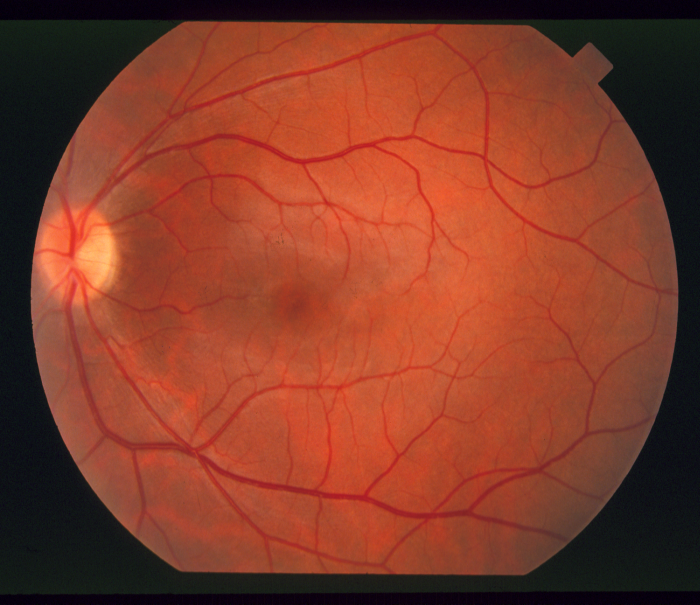
\includegraphics[width=0.3\columnwidth]{figs/retina/17_stare} &
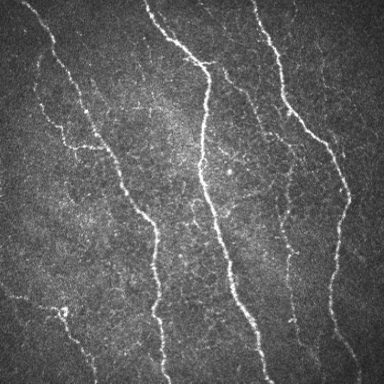
\includegraphics[width=0.3\columnwidth]{figs/fibre/04_fibre_ccm} \\
(a) & (b) & (c) \\
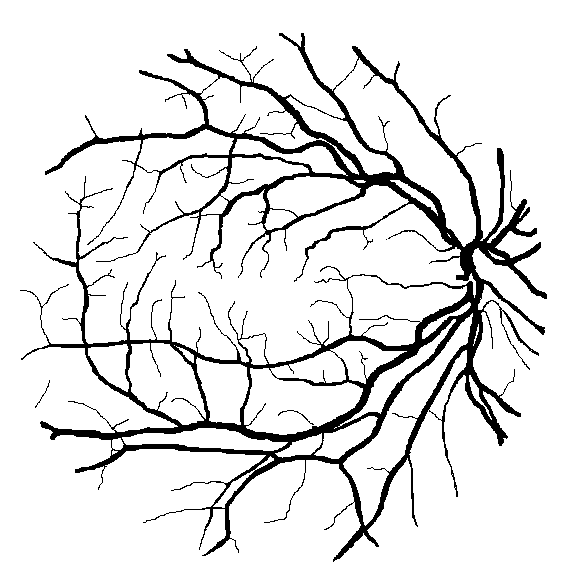
\includegraphics[width=0.3\columnwidth]{figs/retina/02_manual1} &
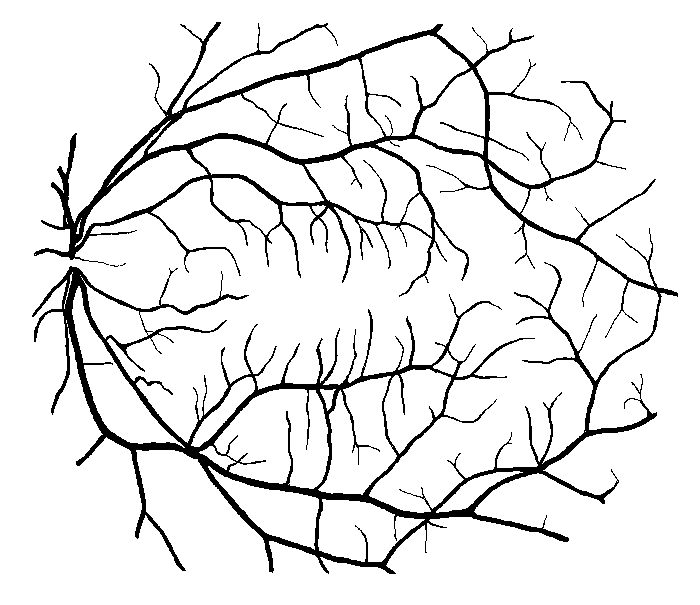
\includegraphics[width=0.3\columnwidth]{figs/retina/17_stare_v_mask} &
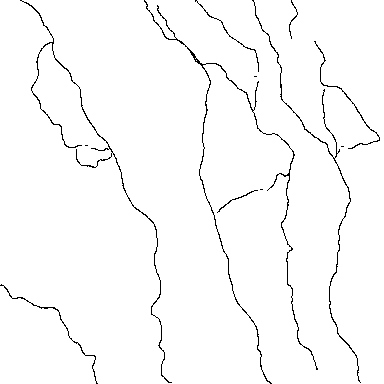
\includegraphics[width=0.3\columnwidth]{figs/fibre/04_fibre_gt} \\
(d) & (e) & (f) \\
\noalign{\smallskip}
\end{tabular}
%
\caption{Example images and their ground truth CLS segmentation: (a,d) DRIVE retinograms; (b,e) STARE retinograms; (c,f)Fibre CCM images }
\label{f:image_examples}
\end{figure}
%
\subsection{DRIVE retinograms}
\label{s:dataset_drive}
The publicly available DRIVE dataset~\cite{Staal_etal_TMI04} contains 40 full colour, JPEG compressed retinogram images (\fref{f:image_examples}a) that originate from a diabetic neuropathy screening program in The Netherlands, where subjects were aged 25-90. The images were acquired using a Canon CR5 non-mydriatic 3CCD camera with a 45 degree field of view (FOV) and 8 bits per colour plane, and are $768 \by 584$ pixels in size. The field of view is defined by a mask, provided with every image, that results in a cropped image $565 \by 584$ pixels in size.

Forty images from a total of 400 were selected for the dataset, seven of which exhibit signs of mild early diabetic retinopathy. These 40 are split into 20 training and 20 test images. Every image comes with at least one mask (test images have two, of which we use the first), hand-labelled by human observers, that define ground truth vessel segmentations (\fref{f:fig_drive_examples}). The segmentations of the training data produce 565,180 vessel and 5,667,260 background pixels, 565,180 vessel and 5,667,260 background pixels in the test images.

Detecting CLS in retinograms enables us to segment the vessel tree from the background. This is useful for diagnosing or quantifying diseases such as diabetic retinopathy, as it enables us either to focus on the vessels (when measuring venous beading or neovascularization, for example) or to ignore the vessels and focus on the background (when counting microaneurysms, haemorrhages and exudates).

The rate of change of orientation (tortuosity) of blood vessels in a retinogram can serve as a diagnostic indicator of vascular disease such as retinopathy of prematurity~\cite{Wallace_TAOS07,Hart_etal_IJMI99}. Though studies suggest that vessels can be detected and segmented~\cite{Staal_etal_TMI04,Ricci_Perfetti_TMI07}, few have addressed the problem of measuring their orientation and quantifying tortuosity.

*We have more text on the clinical importance of retinograms as a means of diagnosing diabetic retinopathy if deemed relevant*

\subsection{STARE retinograms}
\label{s:dataset_stare}
The second set of data we use is the publicly available STARE set of retinograms, compiled by Hoover et al. \cite{Hoover_etal_TMI00}. STARE contains 20 images, which unlike DRIVE, are not split into separate training and test sets. The images are digitised from slides acquired from a TopCon TRV-50 fundus camera at 35 field of view. Each image is encoded with 8 bits per colour plane, and are $700 \by 605$ pixels in size. Ten of the images contain pathology.

A field-of-view of approximately 600 pixels in diameter is clearly identifiable in each image, (\fref{f:image_examples}(b)), however definitive masks are not provided with the original data. We create our own masks by setting a threshold of $40$ in the red channel to remove the dark background outside the field-of-view. We note however that Hoover et al. measured performance using the whole image, whilst others have used their own masks without describing exactly how they are generated \cite{Staal_etal_TMI04} and in some cases, whether masks were used or not is not specified \cite{}. Because the edge of the field-of-view is a common source of false positives, ambiguity in which pixels in this region are included makes a direct comparison to earlier works difficult. The field-of-view masks we use are available from *are we allowed to do this?*.

Two manual segmentations are provided with the images - we use the first observer (labelled as ? in \cite{Hoover_etal_TMI00}) in our experiments. Combined with our field-of-view masks, the segmentations produce 644,000 vessel and 5,592,658 background pixels.

\subsection{Fibre CCM images}
\label{s:dataset_fibre}

Corneal confocal microscopy (CCM) is a non-invasive technique for imaging small nerve fibres in the cornea. Analysis of these fibres, may allow for early damage to be detected and quantified, thus providing a hugely useful clinical tool in diagnosing and assessing the progress of diabetic neuropathy \cite{Dabbah_etal_MICCAI10,Dabbah_etal_MIA11}.

Nerve fibres appears a bright CLS in CCM images, as seen \fref{f:image_examples}(c). Usually there is an approximate dominant orientation of fibres within each image, although individual fibres have locally varying orientation, and may branch or join with neighbouring fibres. The fibres have varying width, and in general, are less well-defined than the vessels in the two retinogram datasets.

We use a set of 200 CCM images, split into a training and test of 100 images each, selected randomly from a larger set of 976 images collected by Dabbah et al. \cite{Dabbah_etal_MICCAI10}. The images were captured with an HRT-III1 microscope, and are $38\times384$ pixels in size, with a spatial resolution of $1.0417\mu m$ per pixel and encoded on an 8-bit grey scale. The images were acquired from a mixture of normal controls and diabetic patients.

The images have been annotated by experts using CCMetrics \cite{}. This provides an approximate centreline for each fibre, as well as a classification between main and secondary fibres and labelling of branch points. Using the marked centrelines, regardless of fibre type, as CLS ground truth provides 240,154 fibre and 14,352,246 background pixels in the training images, and 314,923 fibre and 14,277,477 background pixels in the test set.

\begin{figure*}[t]
\centering
\begin{tabular}{@{}c c c c c@{}} % @{} removes padding around the edge of the table
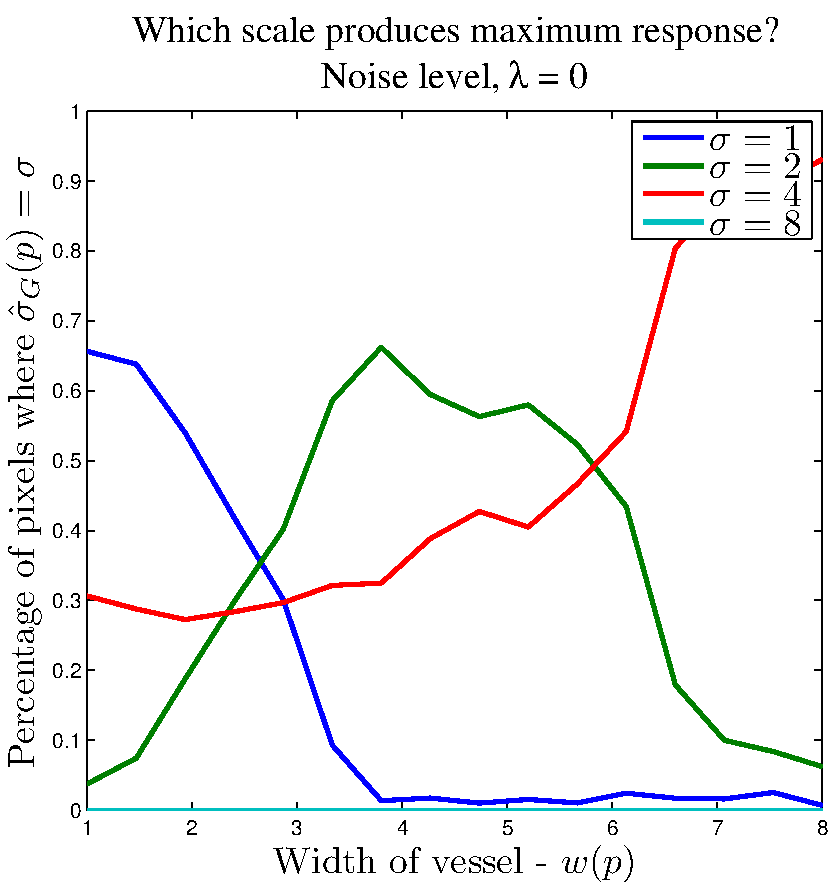
\includegraphics[width=0.18\textwidth]{figs/synthetic/syn_lines_g2d_scales_0} &
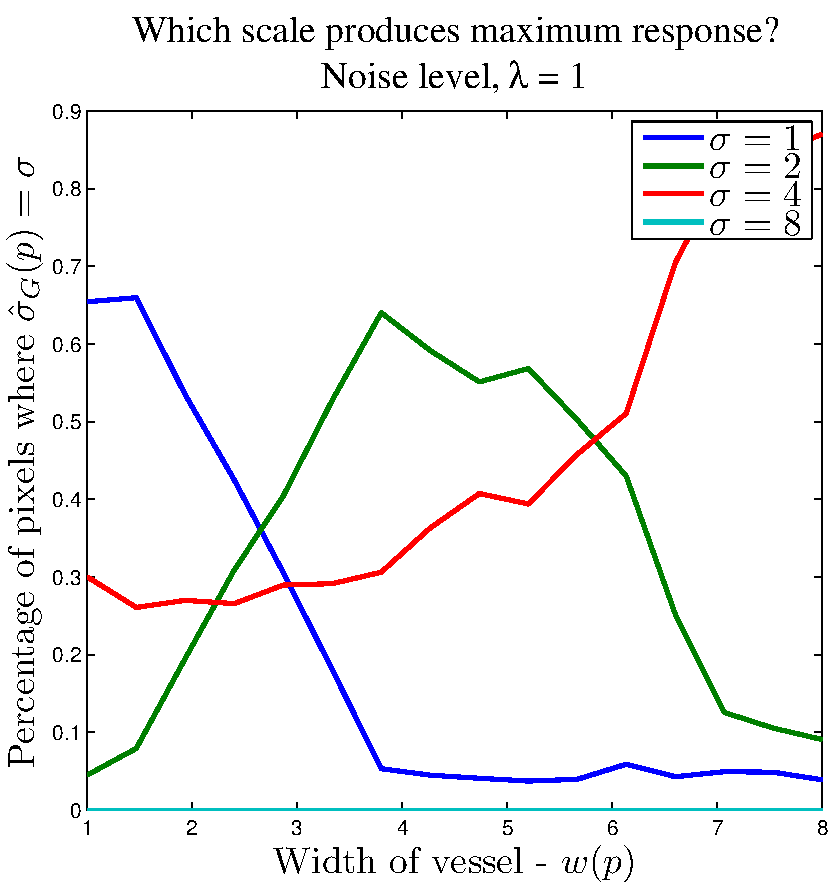
\includegraphics[width=0.18\textwidth]{figs/synthetic/syn_lines_g2d_scales_1} &
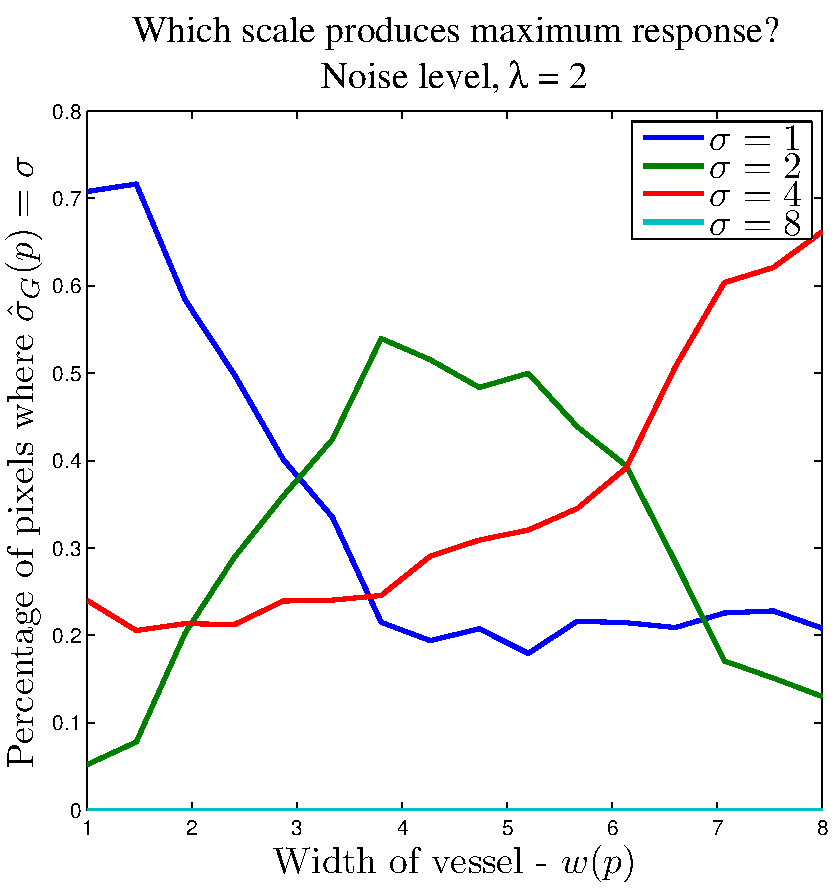
\includegraphics[width=0.18\textwidth]{figs/synthetic/syn_lines_g2d_scales_2} &
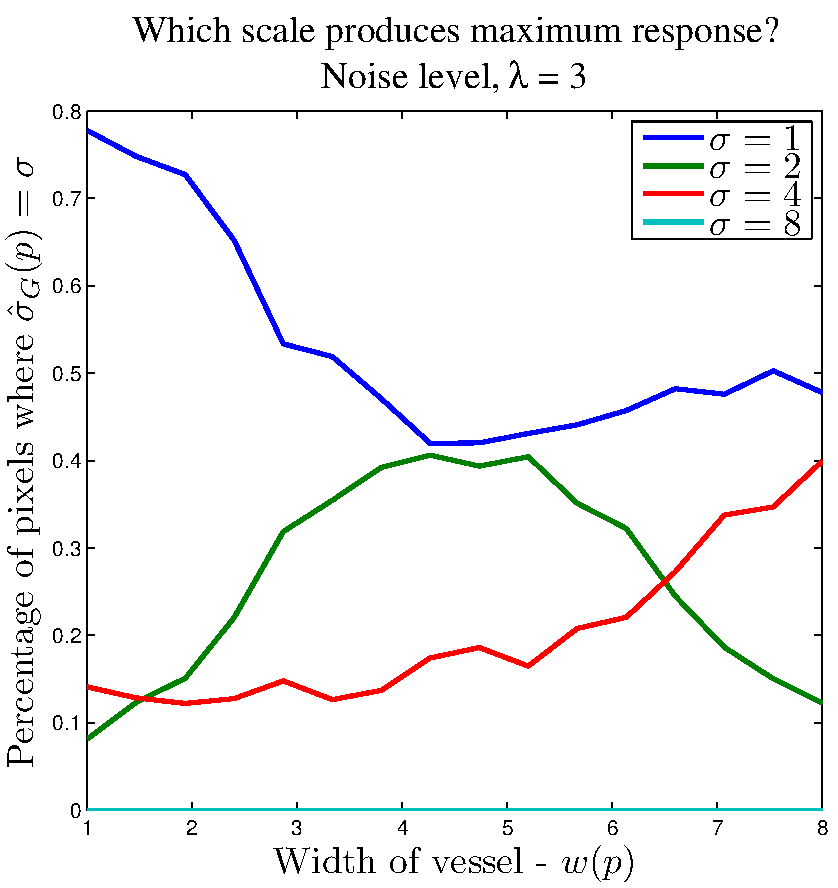
\includegraphics[width=0.18\textwidth]{figs/synthetic/syn_lines_g2d_scales_3} &
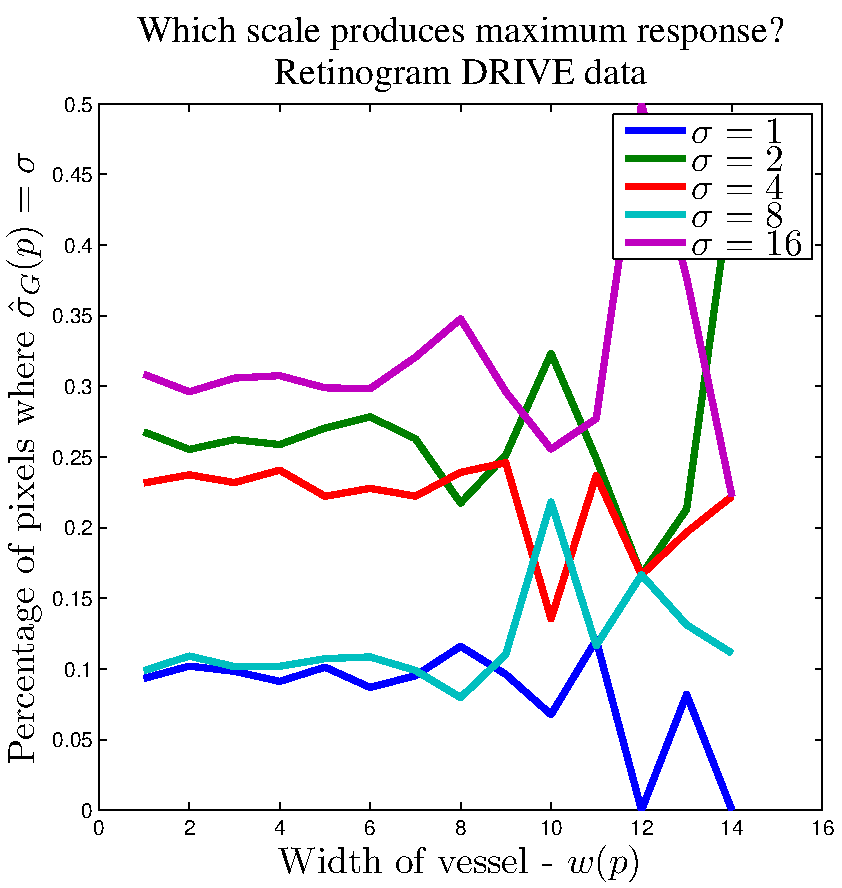
\includegraphics[width=0.18\textwidth]{figs/retina/ret_vessels_g2d_scales} \\
(a) & (b) & (c) & (d) & (e)\\
\noalign{\smallskip}

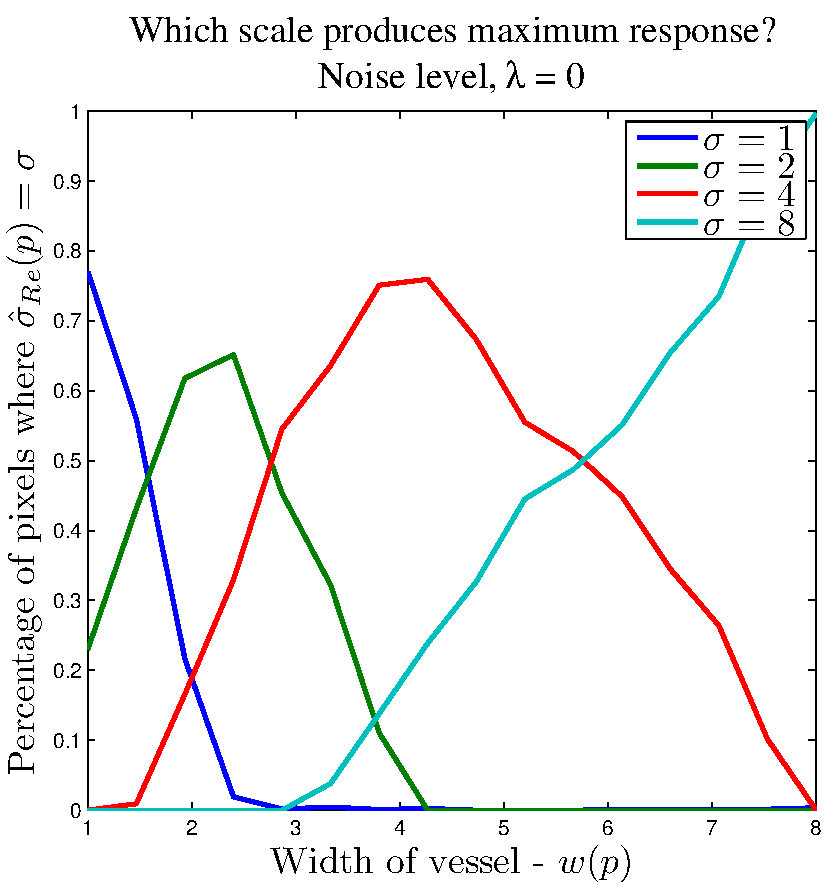
\includegraphics[width=0.18\textwidth]{figs/synthetic/syn_lines_gabor_scales_0} &
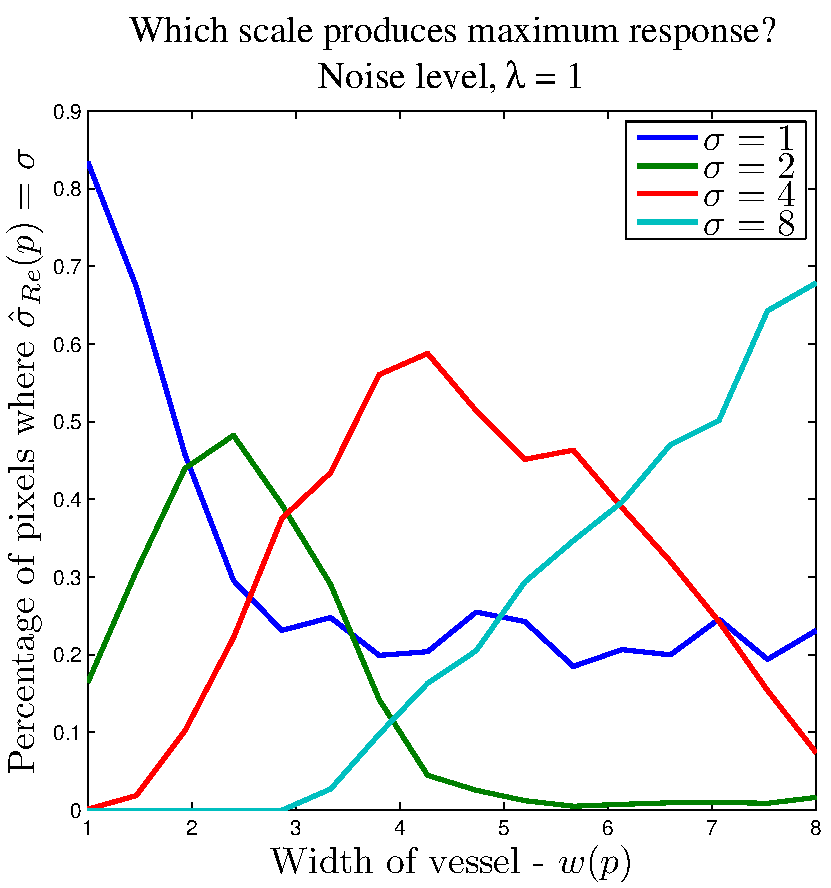
\includegraphics[width=0.18\textwidth]{figs/synthetic/syn_lines_gabor_scales_1} &
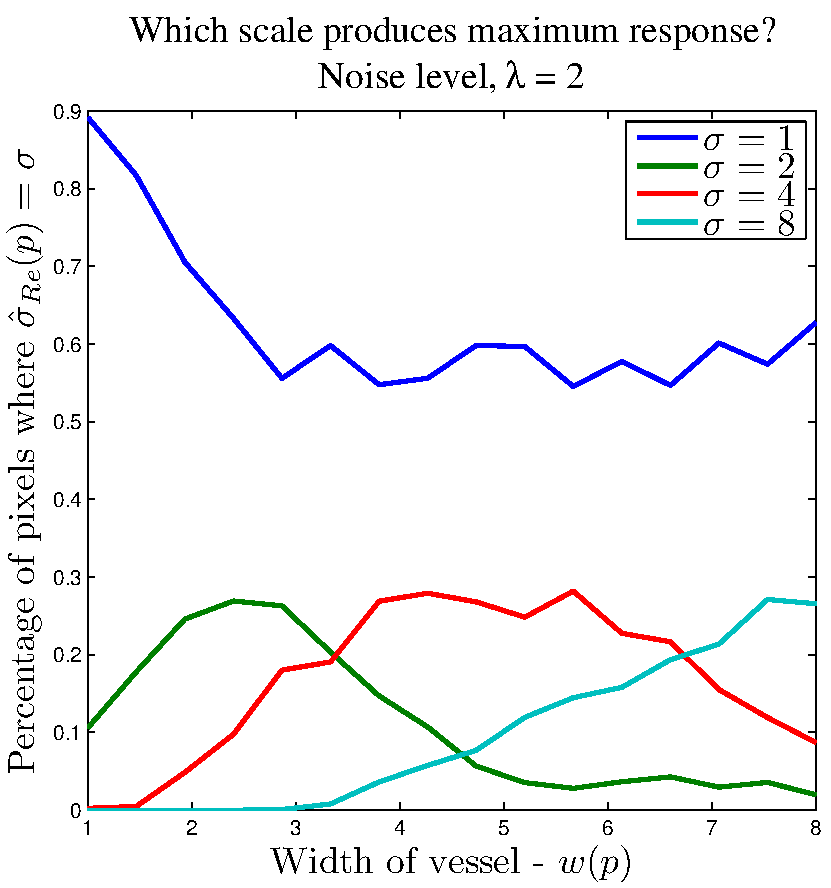
\includegraphics[width=0.18\textwidth]{figs/synthetic/syn_lines_gabor_scales_2} &
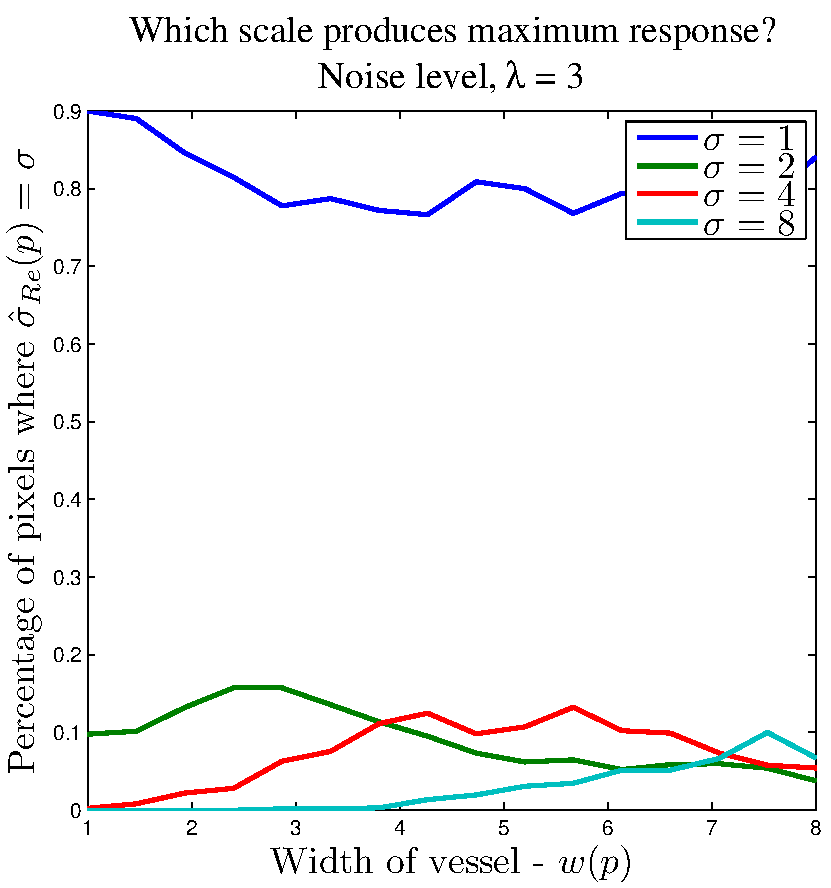
\includegraphics[width=0.18\textwidth]{figs/synthetic/syn_lines_gabor_scales_3} &
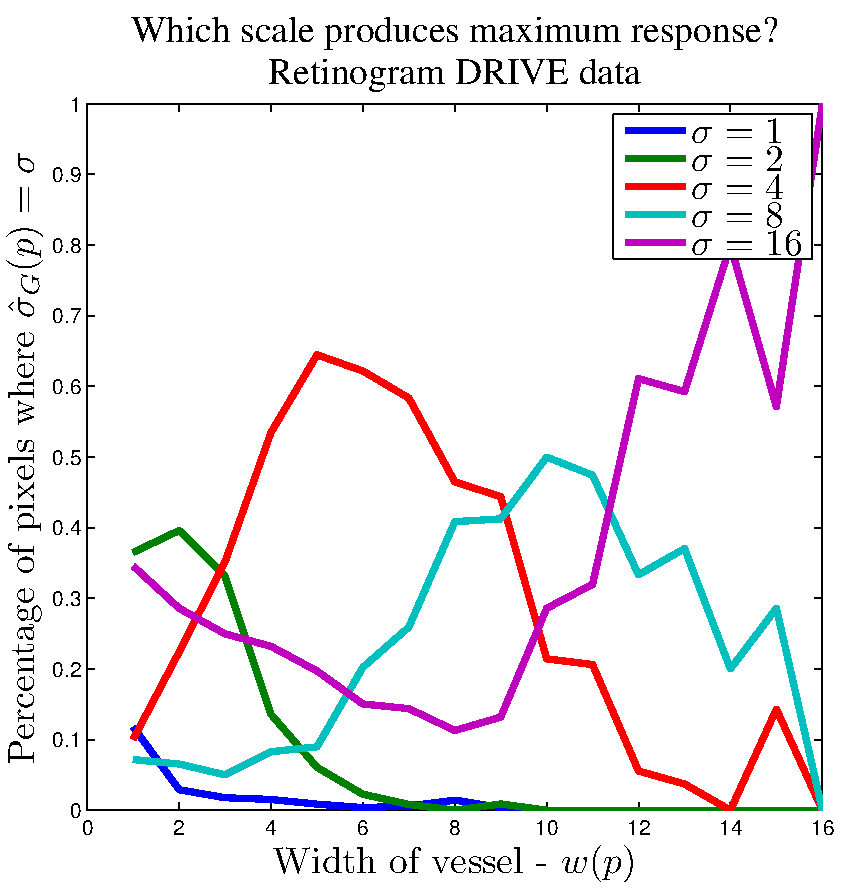
\includegraphics[width=0.18\textwidth]{figs/retina/ret_vessels_gabor_scales} \\
(f) & (g) & (h) & (i) & (j)\\
\noalign{\smallskip}

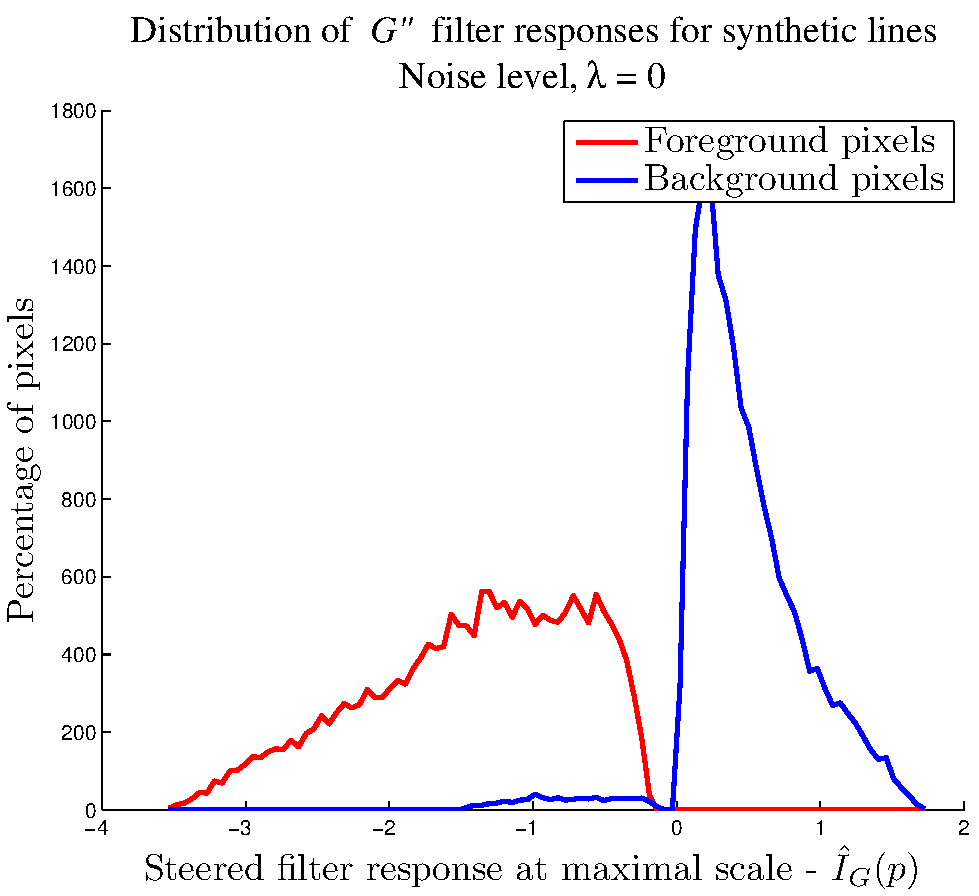
\includegraphics[width=0.18\textwidth]{figs/synthetic/syn_lines_g2d_responses_cdf_0} &
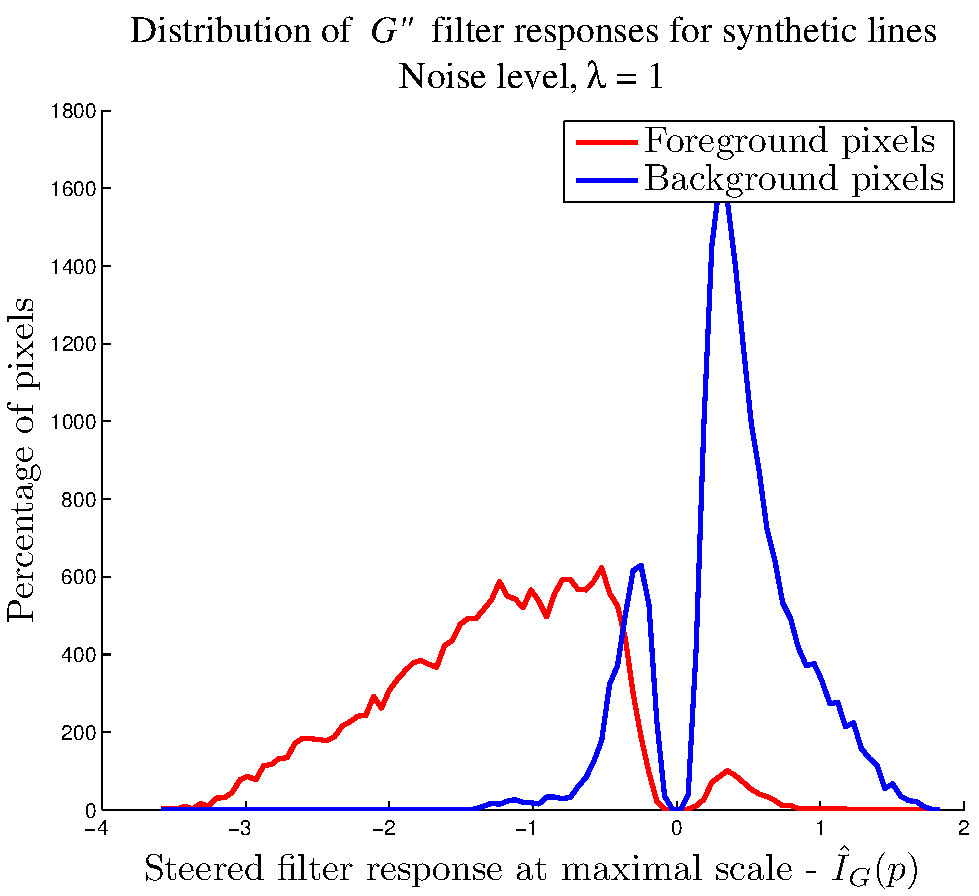
\includegraphics[width=0.18\textwidth]{figs/synthetic/syn_lines_g2d_responses_cdf_1} &
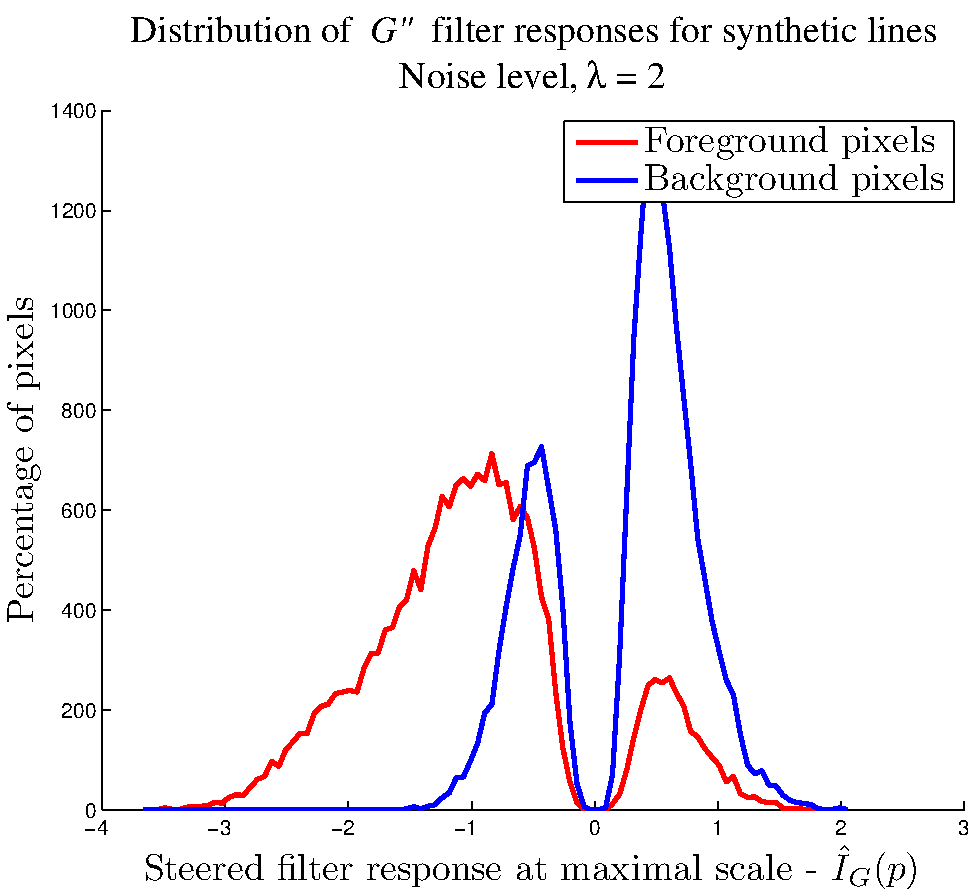
\includegraphics[width=0.18\textwidth]{figs/synthetic/syn_lines_g2d_responses_cdf_2} &
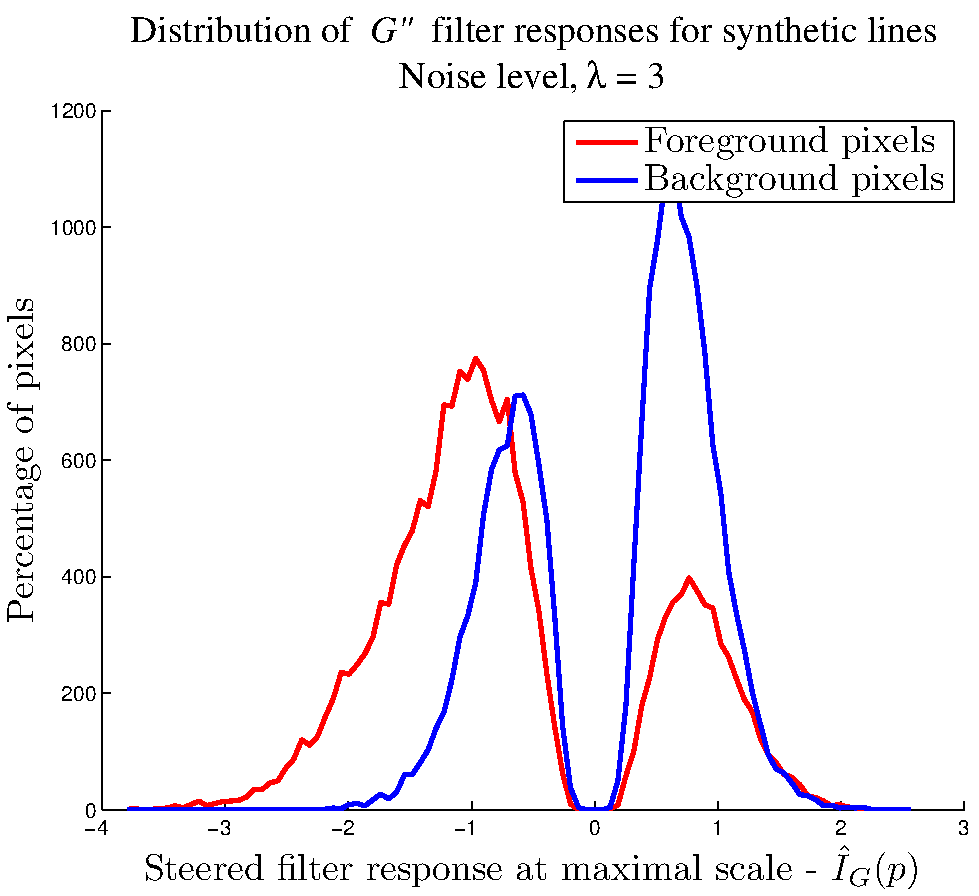
\includegraphics[width=0.18\textwidth]{figs/synthetic/syn_lines_g2d_responses_cdf_3} &
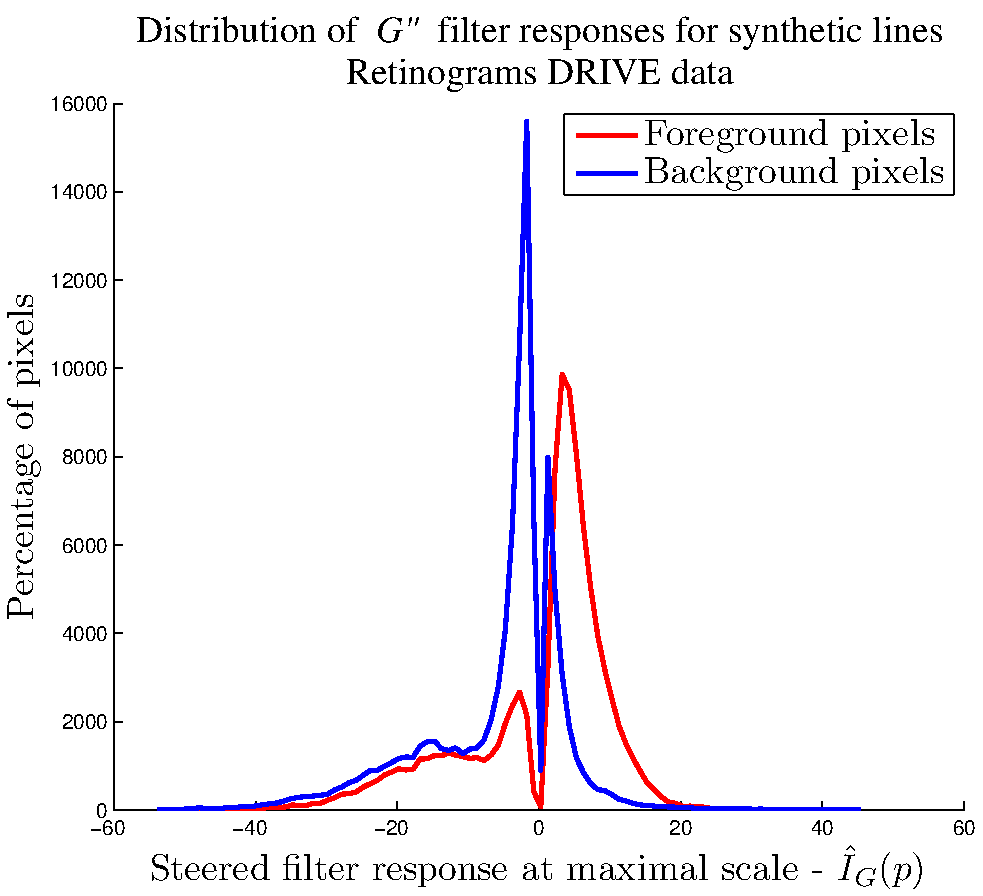
\includegraphics[width=0.18\textwidth]{figs/retina/ret_vessels_g2d_responses_cdf}  \\
(k) & (l) & (m) & (n) & (o)\\
\noalign{\smallskip}

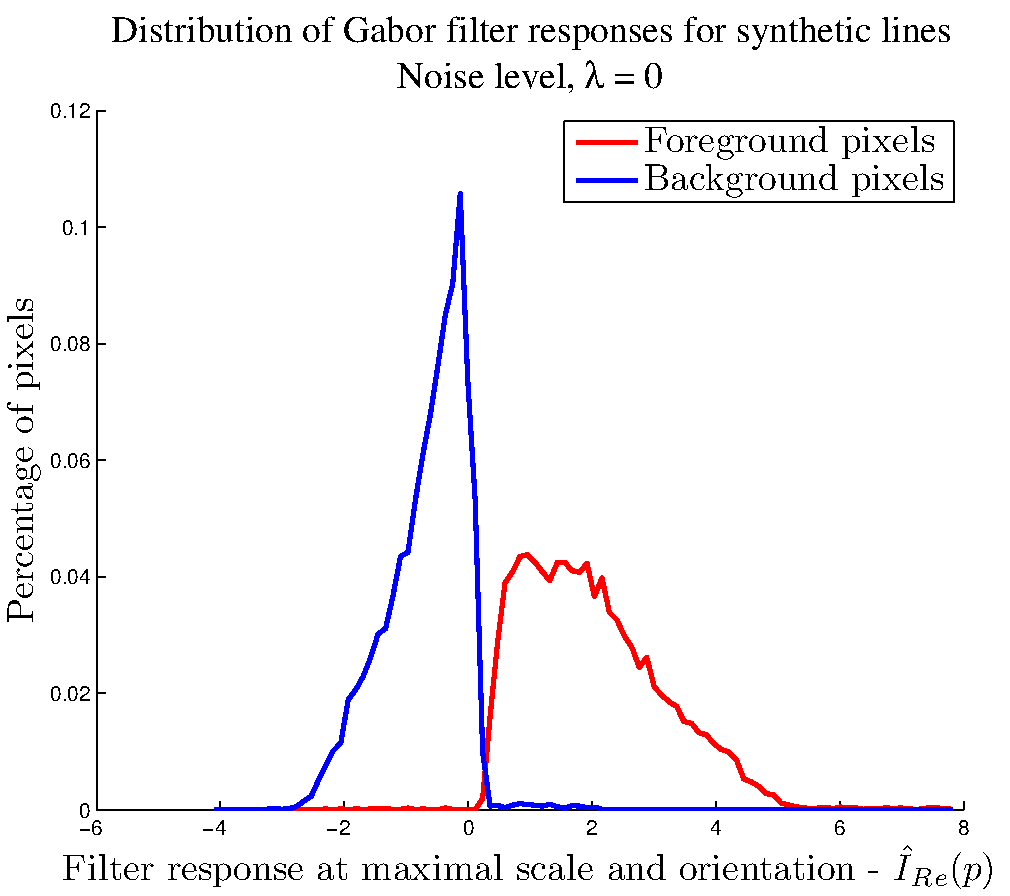
\includegraphics[width=0.18\textwidth]{figs/synthetic/syn_lines_gabor_responses_cdf_0} &
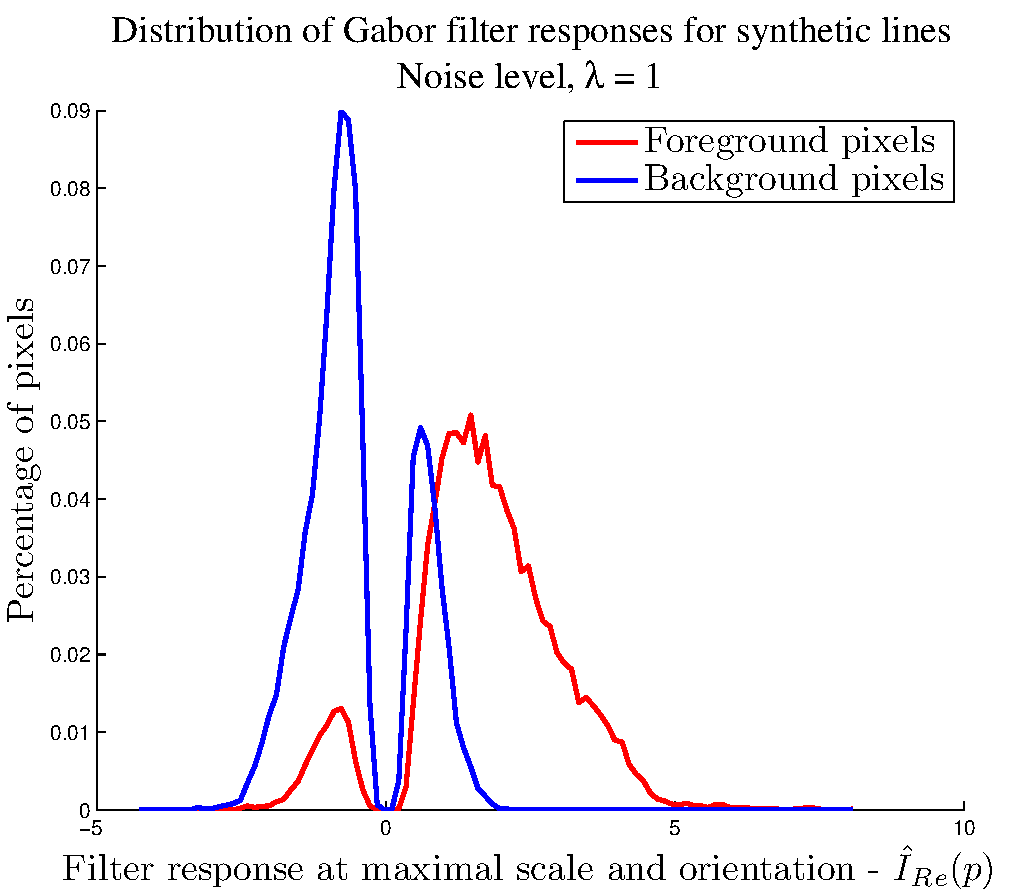
\includegraphics[width=0.18\textwidth]{figs/synthetic/syn_lines_gabor_responses_cdf_1} &
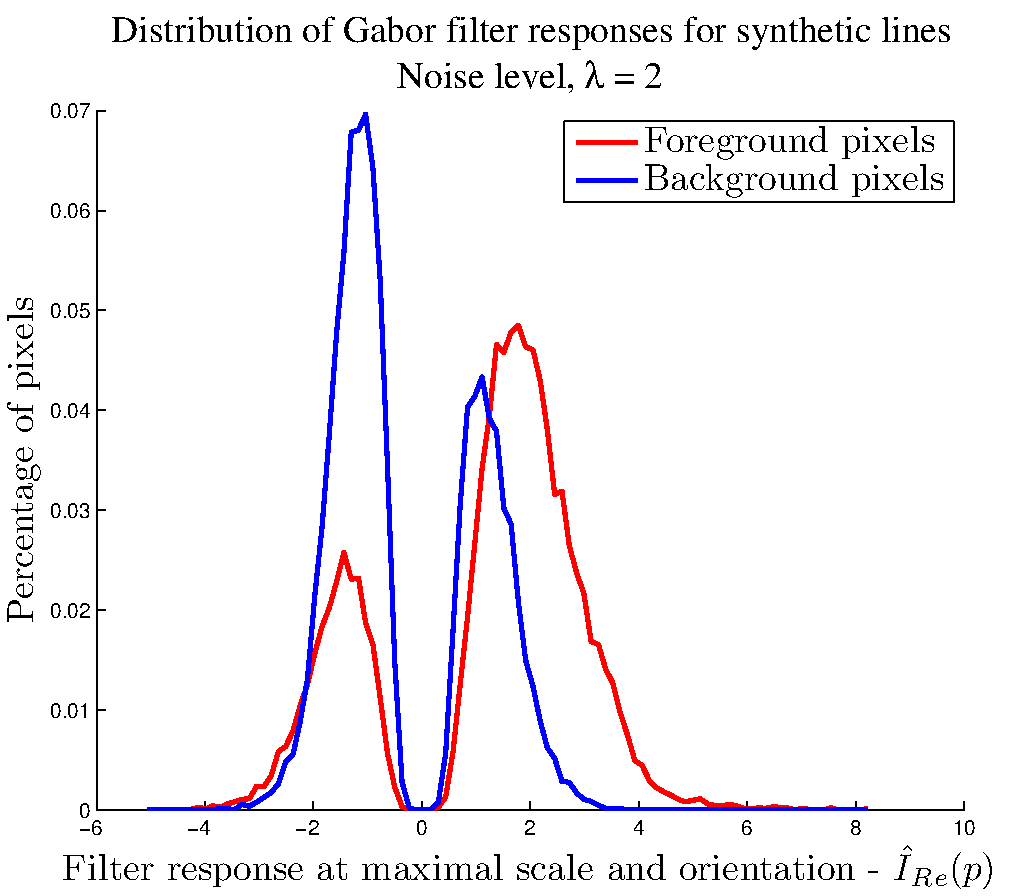
\includegraphics[width=0.18\textwidth]{figs/synthetic/syn_lines_gabor_responses_cdf_2} &
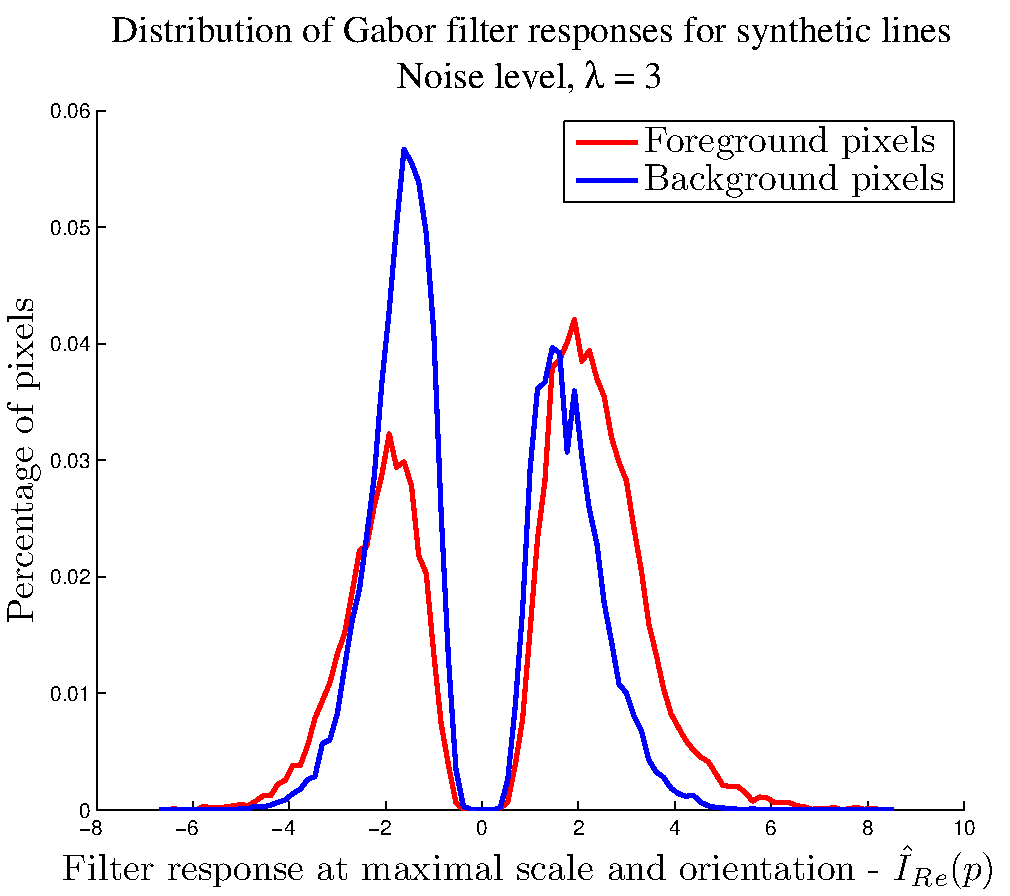
\includegraphics[width=0.18\textwidth]{figs/synthetic/syn_lines_gabor_responses_cdf_3} &
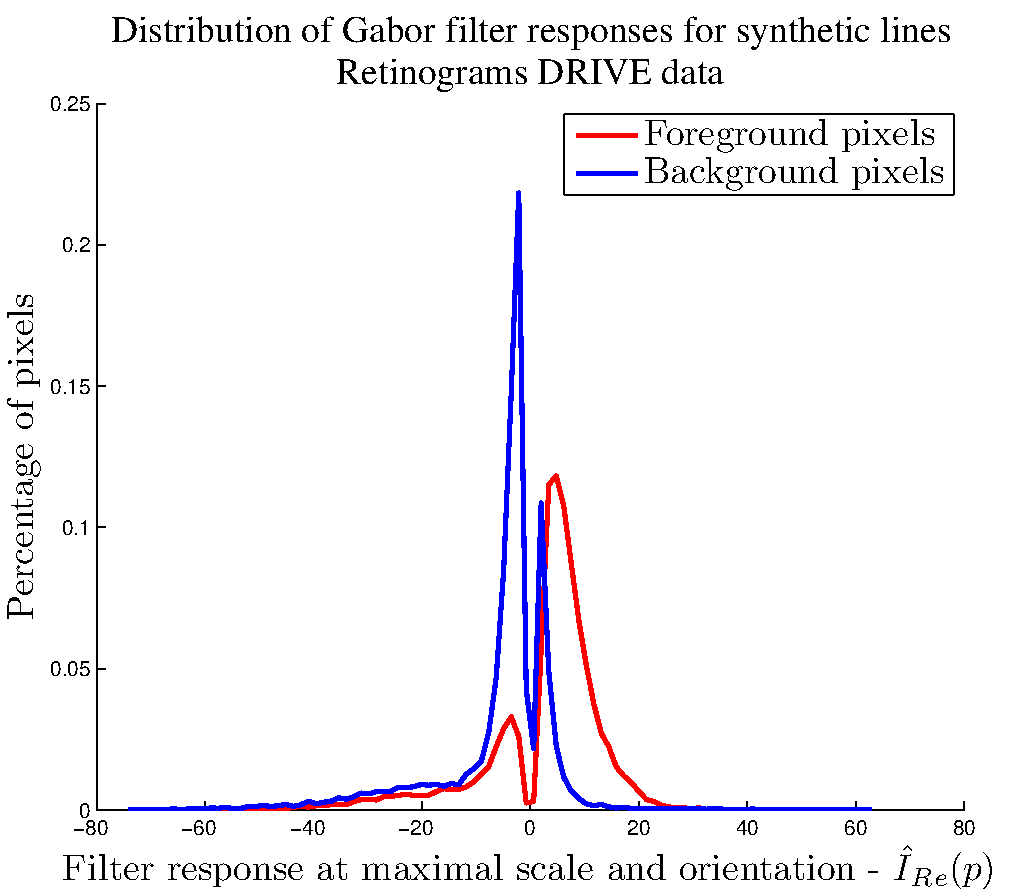
\includegraphics[width=0.18\textwidth]{figs/retina/ret_vessels_gabor_responses_cdf} \\
(p) & (q) & (r) & (s) & (t)\\
\noalign{\smallskip}

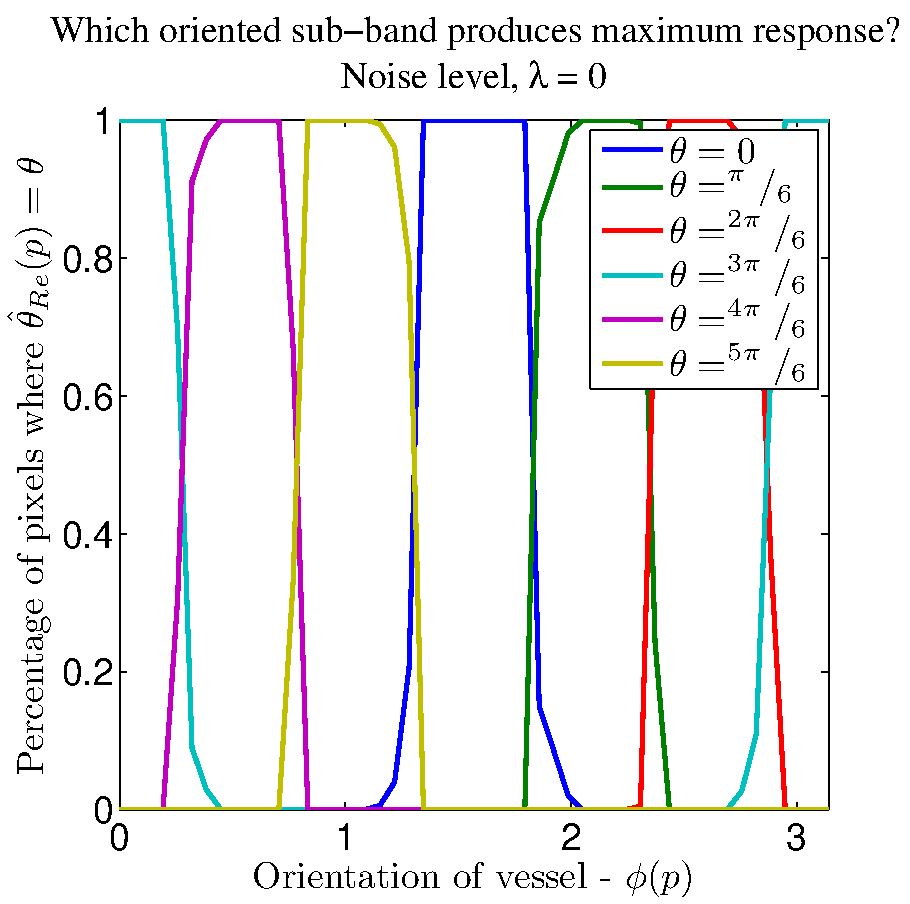
\includegraphics[width=0.18\textwidth]{figs/synthetic/syn_lines_gabor_ori_subbands_0} &
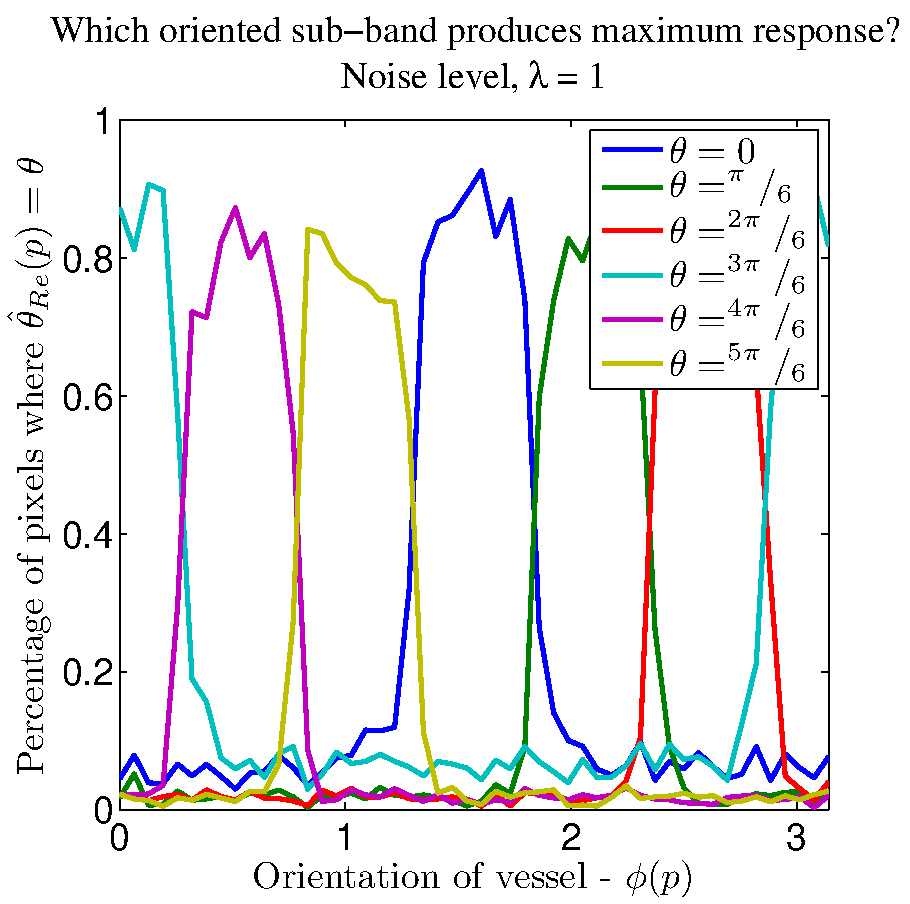
\includegraphics[width=0.18\textwidth]{figs/synthetic/syn_lines_gabor_ori_subbands_1} &
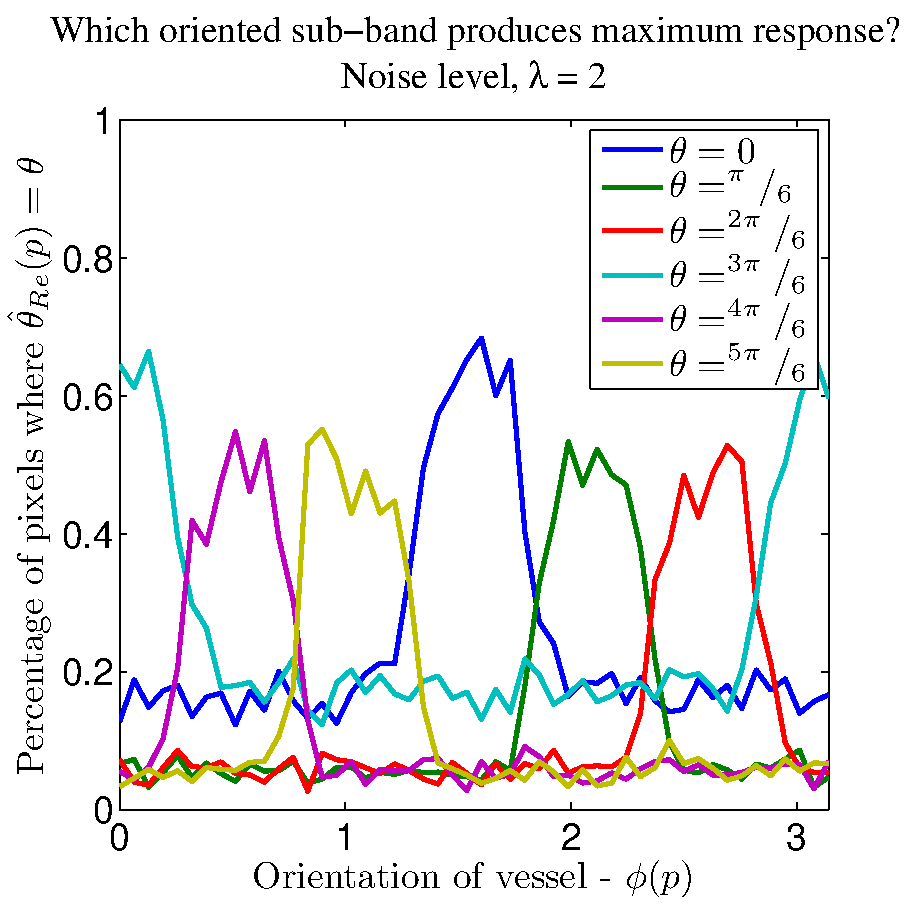
\includegraphics[width=0.18\textwidth]{figs/synthetic/syn_lines_gabor_ori_subbands_2} &
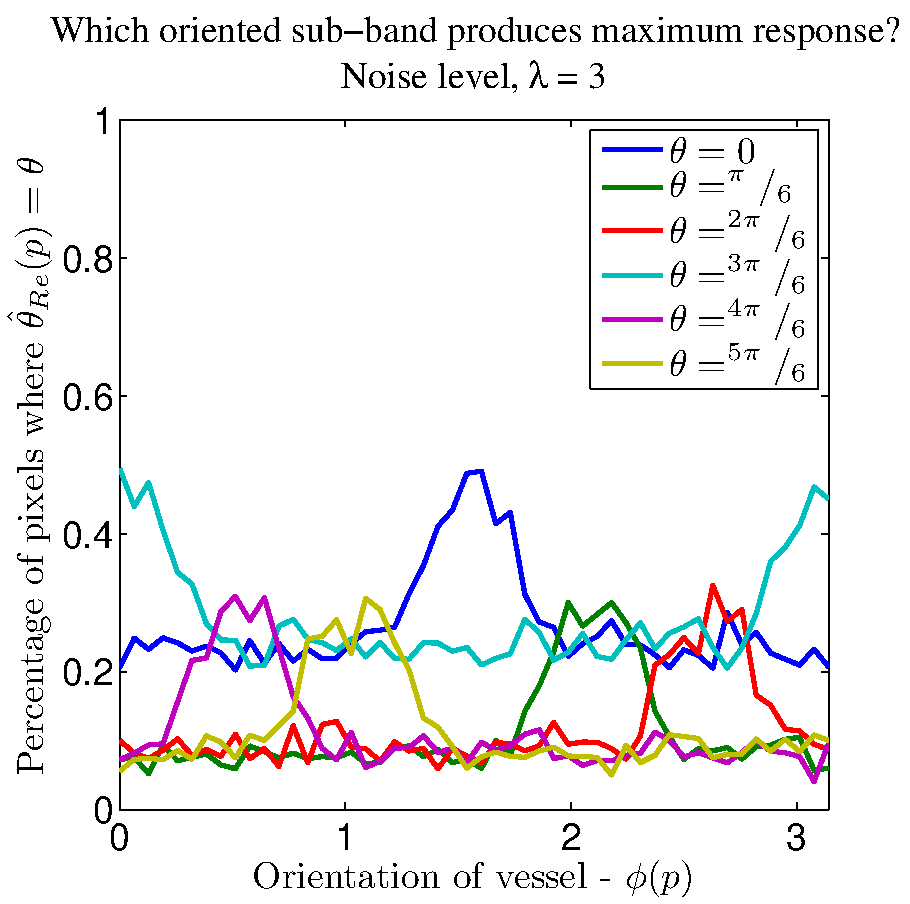
\includegraphics[width=0.18\textwidth]{figs/synthetic/syn_lines_gabor_ori_subbands_3} &
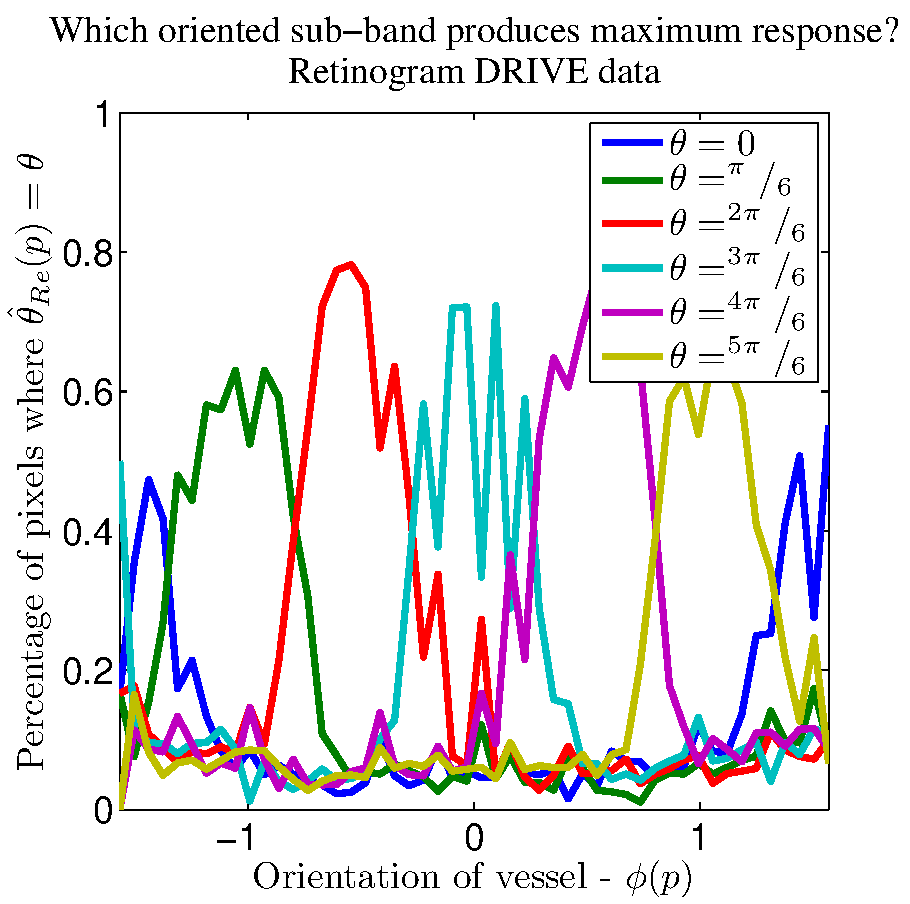
\includegraphics[width=0.18\textwidth]{figs/retina/ret_vessels_gabor_ori_subbands} \\
(u) & (v) & (w) & (x) & (y)\\
\noalign{\smallskip}

\end{tabular}
%
\caption{\emph{Columns from left to right} show results for different datasets: (a-d) synthetic images with noise level of $\eta$ set to 0, 1, 2 and 3 respectively; (e) DRIVE retinograms. Rows top to bottom show: Scale response as a function of CLS width to Gaussian filters(a-e) and Gabor filters (f-j); CLS and background response distribution for Gaussian filters (k-o) and Gabor filters (p-t); Gabor filter response as a function of CLS orientation (u-y).}
\label{f:synthetic_exp1}
\end{figure*}
%
\begin{table*}[t]
\centering
\small
\begin{tabularx}{\linewidth}{p{3.1cm} p{3cm} r r r r r}
\toprule
\multicolumn{7}{l}{DRIVE data} \\
\midrule
            &
            & $w$
            & Size
            & Time
            & \multicolumn{1}{c}{Vessel Detection \linebreak ($A_z$)}
            & \multicolumn{1}{c}{Vessel Orientation \linebreak ($MedAE$)}  \\

\midrule
\multirow{6}{3.1cm}{\centering
    \textbf{Gaussian}
    \newline separable filters,
    \newline
    \newline $\Gxxs$,..., $H_a(\sigma),...$
    \newline  $\sigma = [1, 2, 4, 8, 16]$ }
        & $G$                       & 1 &  15   &  3    & 0.947 $\pm$ 6.4   & 6.89 $\pm$ 0.042 \\
        & $H$                       & 1 &  20   &  4    & 0.838 $\pm$11.0   &10.67 $\pm$ 0.046 \\
        & $G, H$                    & 1 &  35   &  7    & 0.958 $\pm$ 6.4   & 6.67 $\pm$ 0.050 \\
        & $G$                       & 3 & 135   &  3    & 0.959 $\pm$ 5.3   & 6.04 $\pm$ 0.037 \\
        & $H$                       & 3 & 180   &  4    & 0.957 $\pm$ 6.4   & 6.62 $\pm$ 0.031 \\
        & $G, H$                    & 3 & 315   &  7    & 0.961 $\pm$ 6.0   & 5.96 $\pm$ 0.028 \\

\midrule
\multirow{10}{3.1cm}{\centering
    \textbf{Gaussian}
    \newline steered responses,
    \newline
    \newline $G_{\theta}(\sigma)$, $H_{\theta}(\sigma)$
    \newline $\sigma = [1, 2, 4, 8, 16]$
    \newline $\theta = [ \nicefrac{i\pi}{N_\theta} ], N_\theta = 6$ }
        & $G$                       & 1 &  30   &  3    & 0.949 $\pm$ 5.0   & 6.71 $\pm$ 0.038 \\
        & $H$                       & 1 &  30   &  4    & 0.838 $\pm$10.8   &10.39 $\pm$ 0.063\\
        & $G,H$                     & 1 &  60   &  7    & 0.959 $\pm$ 5.7   & 6.46 $\pm$ 0.031 \\
        & $G$                       & 3 & 270   &  4    & 0.961 $\pm$ 5.5   & 5.91 $\pm$ 0.022 \\
        & $H$                       & 3 & 270   &  5    & 0.956 $\pm$ 5.7   & 6.55 $\pm$ 0.029 \\
        & $G,H$                     & 3 & 540   &  9    & 0.962 $\pm$ 5.8   & 5.85 $\pm$ 0.026 \\
        & $Mag$                     & 3 & 270   & 11    & 0.932 $\pm$ 7.6   & 5.82 $\pm$ 0.023 \\
        & $Phase$                   & 3 & 270   & 11    & 0.925 $\pm$ 6.5   & 6.50 $\pm$ 0.043 \\
        & $Mag, Phase$              & 3 & 540   & 11    & 0.961 $\pm$ 5.6   & 5.73 $\pm$ 0.015 \\
        & $\mathbf{Mag, Phase{^*}}$ & \textbf{3} & \textbf{540} & \textbf{11} & \textbf{0.962 $\pm$ 4.7} & \textbf{5.68 $\pm$ 0.020} \\
        & \hspace{2mm} \ldots rotated
                                    & 3 & 540   & 11    & 0.960 $\pm$ 5.4   & --- \\
        & \hspace{2mm} \ldots interpolated
                                    & 3 & 540   &  2    & 0.959 $\pm$ 4.6   & 6.06 $\pm$ 0.034 \\
        & \hspace{2mm} \ldots $N_\theta = 18$
                                    & 3 &1620   & 32    & 0.962 $\pm$ 4.6   & 5.62 $\pm$ 0.027 \\
        & \hspace{2mm} \ldots ${\sigma = [1,...,16]}$
                                    & 3 &1728   & 48    & 0.962 $\pm$ 4.7   & 5.58 $\pm$ 0.025 \\

        & \hspace{2mm} \ldots ${\sigma = 1}$
                                    & 3 & 108   &${<}1$ & 0.941 $\pm$ 7.0   & 6.61 $\pm$ 0.030 \\
        & \hspace{2mm} \ldots ${\sigma = 2}$
                                    & 3 & 108   &${<}1$ & 0.949 $\pm$ 6.3   & 5.87 $\pm$ 0.032 \\
        & \hspace{2mm} \ldots ${\sigma = 4}$
                                    & 3 & 108   &  1    & 0.916 $\pm$ 4.9   & 7.51 $\pm$ 0.037 \\
        & \hspace{2mm} \ldots ${\sigma = 8}$
                                    & 3 & 108   &  2    & 0.820 $\pm$11.0   &13.80 $\pm$ 0.055 \\


\midrule
\multirow{14}{3.1cm}{\centering
    \textbf{Gabor}
    \newline oriented filters,
    \newline
    \newline $W_{re}(\sigma,\theta)$, $W_{im}(\sigma,\theta)$
    \newline $\sigma = [1, 2, 4, 8, 16]$
    \newline $\theta = [ \nicefrac{i\pi}{N_\theta} ], N_\theta = 6$ }
        & $Re$                      & 1 &  30   & 82    & 0.948 $\pm$ 6.0   & 6.15 $\pm$ 0.033 \\
        & $Im$                      & 1 &  30   & 82    & 0.854 $\pm$ 1.2   & 8.08 $\pm$ 0.041 \\
        & $Re,Im$                   & 1 &  60   &164    & 0.959 $\pm$ 5.5   & 5.82 $\pm$ 0.027 \\
        & $Re$                      & 3 & 270   & 82    & 0.960 $\pm$ 5.7   & 5.47 $\pm$ 0.021 \\
        & $Im$                      & 3 & 270   & 82    & 0.953 $\pm$ 6.5   & 5.52 $\pm$ 0.024 \\
        & $Re,Im$                   & 3 & 540   &164    & 0.962 $\pm$ 5.7   & 5.34 $\pm$ 0.019 \\
        & $Mag$                     & 3 & 270   &164    & 0.932 $\pm$ 8.6   & 4.92 $\pm$ 0.023 \\
        & $Phase$                   & 3 & 270   &164    & 0.912 $\pm$ 8.6   & 9.38 $\pm$ 0.059 \\
        & $Mag,Phase$               & 3 & 540   &164    & 0.959 $\pm$ 5.9   & 4.93 $\pm$ 0.015 \\
        & $\mathbf{Mag, Phase{^*}}$ & \textbf{3} & \textbf{540} &\textbf{164} & \textbf{0.962 $\pm$ 6.6} & \textbf{4.85 $\pm$ 0.020} \\
        & \hspace{2mm} \ldots rotated
                                    & 3 & 540   &164    & 0.963 $\pm$ 4.7   & --- \\
        & \hspace{2mm} \ldots interpolated
                                    & 3 & 540   &  7    & 0.959 $\pm$ 5.0   & 5.44 $\pm$ 0.022 \\
        & \hspace{2mm} \ldots $N_\theta = 18$
                                    & 3 &1620   &493    & 0.963 $\pm$ 5.8   & 4.74 $\pm$ 0.021 \\
        & \hspace{2mm} \ldots ${\sigma = [1,...,16]}$
                                    & 3 &1728   &553    & 0.963 $\pm$ 5.5   & 4.59 $\pm$ 0.017 \\

        & \hspace{2mm} \ldots ${\sigma = 1}$
                                    & 3 & 108   &  6    & 0.921 $\pm$ 9.5   & 9.27 $\pm$ 0.033 \\
        & \hspace{2mm} \ldots ${\sigma = 2}$
                                    & 3 & 108   & 11    & 0.952 $\pm$ 6.9   & 5.89 $\pm$ 0.022 \\
        & \hspace{2mm} \ldots ${\sigma = 4}$
                                    & 3 & 108   & 22    & 0.946 $\pm$ 4.7   & 5.00 $\pm$ 0.015 \\
        & \hspace{2mm} \ldots ${\sigma = 8}$
                                    & 3 & 108   & 43    & 0.900 $\pm$ 4.5   & 7.09 $\pm$ 0.040 \\

\midrule
\multirow{14}{3.1cm}{\centering
    \textbf{\dtcwt{}}
    \newline 5 levels
    \newline 6 oriented sub-bands }
        & $Re$                      & 1 &  30   &${<}1$ & 0.920 $\pm$ 7.7   & 7.08 $\pm$ 0.026 \\
        & $Im$                      & 1 &  30   &${<}1$ & 0.900 $\pm$ 6.9   & 7.76 $\pm$ 0.046 \\
        & $Re,Im$                   & 1 &  60   &  1    & 0.952 $\pm$ 5.6   & 5.92 $\pm$ 0.024 \\
        & $Re$                      & 3 & 270   &  1    & 0.951 $\pm$ 6.1   & 5.78 $\pm$ 0.023 \\
        & $Im$                      & 3 & 270   &  1    & 0.951 $\pm$ 6.6   & 5.70 $\pm$ 0.028 \\
        & $Re,Im$                   & 3 & 540   &  2    & 0.956 $\pm$ 5.9   & 5.51 $\pm$ 0.027 \\
        & $Mag$                     & 3 & 270   &  2    & 0.918 $\pm$ 7.2   & 5.05 $\pm$ 0.020 \\
        & $Phase$                   & 3 & 270   &  2    & 0.879 $\pm$ 7.9   & 10.8 $\pm$ 0.063 \\
        & $Mag,Phase$               & 3 & 540   &  2    & 0.955 $\pm$ 5.9   & 4.98 $\pm$ 0.026 \\
        & $\mathbf{Mag, Phase{^*}}$ & \textbf{3} & \textbf{540}   & \textbf{2}    & \textbf{0.953 $\pm$ 5.9}   & \textbf{4.96 $\pm$ 0.024} \\
        & \hspace{2mm} \ldots rotated
                                    & 3 & 540   &  2    & 0.946 $\pm$ 6.0   & --- \\

\midrule
\multirow{2}{3.1cm}{\centering
    \textbf{Monogenic Signal}
    \newline A, $\psi$, $\theta$
    \newline 5 levels}

                                   && \textbf{3} & \textbf{135} &  \textbf{5} & \textbf{0.951 $\pm$ 5.5} & \textbf{7.85 $\pm$ 0.045} \\
                                   &&   &       &       &                   & \\
\midrule
\multicolumn{1}{c}{\textbf{All filters}}
                                   && 3 & 1755  &???    & 0.964 $\pm$ 5.0   & 4.63 $\pm$ 0.024 \\
                                   &&   &       &       &                   & \\

\bottomrule
\noalign{\smallskip}
\end{tabularx}

\caption{Detecting and predicting the orientation of retinal vessels. DRIVE database, training images, all feature vector permutations (features in bold subsequently used to predict test images)}
\label{t:drive_training_c}
\end{table*}
%
\begin{table*}[t]
\centering
\small
\begin{tabularx}{\linewidth}{p{3.1cm} p{3cm} r r r r r}
\toprule
\multicolumn{7}{l}{Fibre data} \\
\midrule
            &
            & $w$
            & Size
            & Time
            & \multicolumn{1}{c}{Vessel Detection \linebreak ($A_z$)}
            & \multicolumn{1}{c}{Vessel Orientation \linebreak ($MedAE$)}  \\

\midrule
\multirow{6}{3.1cm}{\centering
    \textbf{Gaussian}
    \newline separable filters,
    \newline
    \newline $\Gxxs$,..., $H_a(\sigma),...$
    \newline  $\sigma = [1, 2, 4, 8, 16]$ }
        & $G$                       & 1 &    15 &   3   & 0.896 $\pm$ 3.2   & 8.82 $\pm$ 0.16 \\
        & $H$                       & 1 &    20 &   4   & 0.819 $\pm$ 1.8   &16.60 $\pm$ 0.47 \\
        & $G, H$                    & 1 &    35 &   7   & 0.901 $\pm$ 3.0   & 8.68 $\pm$ 0.17 \\
        & $G$                       & 3 &   135 &   3   & 0.902 $\pm$ 3.2   & 8.43 $\pm$ 0.17 \\
        & $H$                       & 3 &   180 &   4   & 0.892 $\pm$ 2.7   & 8.98 $\pm$ 0.24 \\
        & $G, H$                    & 3 &   315 &   7   & 0.903 $\pm$ 3.0   & 8.32 $\pm$ 0.17 \\

\midrule
\multirow{10}{3.1cm}{\centering
    \textbf{Gaussian}
    \newline steered responses,
    \newline
    \newline $G_{\theta}(\sigma)$, $H_{\theta}(\sigma)$
    \newline $\sigma = [1, 2, 4, 8, 16]$
    \newline $\theta = [ \nicefrac{i\pi}{N_\theta} ], N_\theta = 6$ }
        & $G$                       & 1 &  30   &  3    & 0.897 $\pm$ 3.2   & 8.76 $\pm$ 0.16 \\
        & $H$                       & 1 &  30   &  4    & 0.820 $\pm$ 1.9   &16.10 $\pm$ 0.43 \\
        & $G,H$                     & 1 &  60   &  7    & 0.901 $\pm$ 3.0   & 8.60 $\pm$ 0.16 \\
        & $G$                       & 3 & 270   &  4    & 0.903 $\pm$ 3.1   & 8.40 $\pm$ 0.16 \\
        & $H$                       & 3 & 270   &  5    & 0.892 $\pm$ 2.8   & 8.85 $\pm$ 0.23 \\
        & $G,H$                     & 3 & 540   &  9    & 0.903 $\pm$ 2.9   & 8.31 $\pm$ 0.16 \\
        & $Mag$                     & 3 & 270   & 11    & 0.876 $\pm$ 2.5   & 8.65 $\pm$ 0.19 \\
        & $Phase$                   & 3 & 270   & 11    & 0.876 $\pm$ 3.5   & 9.34 $\pm$ 0.21 \\
        & $Mag, Phase$              & 3 & 540   & 11    & 0.901 $\pm$ 2.8   & 8.27 $\pm$ 0.19 \\
        & $\mathbf{Mag, Phase{^*}}$ & \textbf{3} & \textbf{540} & \textbf{11} & \textbf{0.903 $\pm$ 3.1} & \textbf{8.15 $\pm$ 0.17} \\
        & \hspace{2mm} \ldots rotated
                                    & 3 & 540   & 11    & 0.900 $\pm$ 2.7   & --- \\
        & \hspace{2mm} \ldots interpolated
                                    & 3 & 540   &  2    & 0.901 $\pm$ 3.1   & 8.57 $\pm$ 0.18 \\
        & \hspace{2mm} \ldots ${\sigma = 1}$
                                    & 3 & 108   &${<}1$ & 0.851 $\pm$ 3.2   &12.40 $\pm$ 0.38 \\
        & \hspace{2mm} \ldots ${\sigma = 2}$
                                    & 3 & 108   &${<}1$ & 0.885 $\pm$ 3.2   & 9.27 $\pm$ 0.23 \\
        & \hspace{2mm} \ldots ${\sigma = 4}$
                                    & 3 & 108   &  1    & 0.893 $\pm$ 3.3   & 8.48 $\pm$ 0.18 \\
        & \hspace{2mm} \ldots ${\sigma = 8}$
                                    & 3 & 108   &  2    & 0.839 $\pm$ 2.9   &11.70 $\pm$ 0.17 \\

\midrule
\multirow{14}{3.1cm}{\centering
    \textbf{Gabor}
    \newline oriented filters,
    \newline
    \newline $W_{re}(\sigma,\theta)$, $W_{im}(\sigma,\theta)$
    \newline $\sigma = [1, 2, 4, 8, 16]$
    \newline $\theta = [ \nicefrac{i\pi}{N_\theta} ], N_\theta = 6$ }
        & $Re$                      & 1 &  30   & 82    & 0.901 $\pm$ 3.1   & 7.92 $\pm$ 0.15 \\
        & $Im$                      & 1 &  30   & 82    & 0.835 $\pm$ 2.2   &13.11 $\pm$ 0.41 \\
        & $Re,Im$                   & 1 &  60   &164    & 0.906 $\pm$ 3.0   & 7.75 $\pm$ 0.15 \\
        & $Re$                      & 3 & 270   & 82    & 0.907 $\pm$ 3.1   & 7.64 $\pm$ 0.13 \\
        & $Im$                      & 3 & 270   & 82    & 0.895 $\pm$ 3.0   & 7.87 $\pm$ 0.23 \\
        & $Re,Im$                   & 3 & 540   &164    & 0.908 $\pm$ 3.0   & 7.51 $\pm$ 0.13 \\
        & $Mag$                     & 3 & 270   &164    & 0.884 $\pm$ 2.5   & 7.23 $\pm$ 0.14 \\
        & $Phase$                   & 3 & 270   &164    & 0.867 $\pm$ 3.6   &10.41 $\pm$ 0.26 \\
        & $Mag,Phase$               & 3 & 540   &164    & 0.905 $\pm$ 3.1   & 7.07 $\pm$ 0.14 \\
        & $\mathbf{Mag, Phase{^*}}$ & \textbf{3} & \textbf{540} &\textbf{164} & \textbf{0.908 $\pm$ 3.0} & \textbf{7.05 $\pm$ 0.13} \\
        & \hspace{2mm} \ldots rotated
                                    & 3 & 540   &164    & 0.906 $\pm$ 2.6   & --- \\
        & \hspace{2mm} \ldots interpolated
                                    & 3 & 540   &  7    & 0.899 $\pm$ 2.9   & 7.93 $\pm$ 0.17 \\
        & \hspace{2mm} \ldots ${\sigma = 1}$
                                    & 3 & 108   &  6    & 0.814 $\pm$ 3.2   &17.00 $\pm$ 0.54 \\
        & \hspace{2mm} \ldots ${\sigma = 2}$
                                    & 3 & 108   & 11    & 0.866 $\pm$ 3.1   &10.50 $\pm$ 0.31 \\
        & \hspace{2mm} \ldots ${\sigma = 4}$
                                    & 3 & 108   & 22    & 0.893 $\pm$ 3.1   & 7.50 $\pm$ 0.18 \\
        & \hspace{2mm} \ldots ${\sigma = 8}$
                                    & 3 & 108   & 43    & 0.887 $\pm$ 3.3   & 7.91 $\pm$ 0.14 \\

\midrule
\multirow{14}{3.1cm}{\centering
    \textbf{\dtcwt{}}
    \newline 5 levels
    \newline 6 oriented sub-bands }
        & $Re$                      & 1 &  30   &${<}1$ & 0.897 $\pm$ 3.0   & 8.07 $\pm$ 0.14 \\
        & $Im$                      & 1 &  30   &${<}1$ & 0.834 $\pm$ 2.4   &13.42 $\pm$ 0.42 \\
        & $Re,Im$                   & 1 &  60   &  1    & 0.902 $\pm$ 3.0   & 7.91 $\pm$ 0.15 \\
        & $Re$                      & 3 & 270   &  6    & 0.903 $\pm$ 3.0   & 7.80 $\pm$ 0.14 \\
        & $Im$                      & 3 & 270   &  6    & 0.891 $\pm$ 3.0   & 8.06 $\pm$ 0.21 \\
        & $Re,Im$                   & 3 & 540   & 12    & 0.905 $\pm$ 2.9   & 7.65 $\pm$ 0.13 \\
        & $Mag$                     & 3 & 270   & 12    & 0.869 $\pm$ 2.2   & 7.49 $\pm$ 0.15 \\
        & $Phase$                   & 3 & 270   & 12    & 0.845 $\pm$ 4.4   &10.69 $\pm$ 0.21 \\
        & $Mag,Phase$               & 3 & 540   & 12    & 0.898 $\pm$ 2.6   & 7.26 $\pm$ 0.16 \\
        & $\mathbf{Mag, Phase{^*}}$ & \textbf{3} & \textbf{540} & \textbf{2} & \textbf{0.902 $\pm$ 2.6} & \textbf{7.19 $\pm$ 0.15} \\
        & \hspace{2mm} \ldots rotated
                                    & 3 & 540   & 12    & 0.899 $\pm$ 2.3   & --- \\

\midrule
\multirow{2}{3.1cm}{\centering
    \textbf{Monogenic Signal}
    \newline A, $\psi$, $\theta$
    \newline 5 levels}

                                   && \textbf{3} & \textbf{135} &  \textbf{5} & \textbf{0.883 $\pm$ 2.5} & \textbf{12.10 $\pm$ 0.35} \\
                                   &&   &       &       &                   & \\
\midrule
\multicolumn{1}{c}{\textbf{All filters}}
                                   && 3 & 1755  &???    & 0.907 $\pm$ 2.5   & 7.05 $\pm$ 0.22 \\
                                   &&   &       &       &                   & \\

\bottomrule
\noalign{\smallskip}
\end{tabularx}

\caption{Detecting and predicting the orientation of nerve fibres in confocal corneal microscopy images. Training images, all feature vector permutations (features in bold subsequently used to predict test images)}
\label{t:fibre_training_c}
\end{table*}

\FloatBarrier

\subsection{Synthetic images}
\label{s:dataset_synthetic}

In addition to real data, we use synthetic images in which we have complete control over the ground truth and level of noise in the images. To generate each synthetic image we add a line with elliptical profile to an empty $64\times64$ pixel background. Both the contrast and width of the lines are sampled uniformly in the range $[1, 8]$, whilst line orientation is sampled uniformly over the circle.

The image is then corrupted Rician noise \cite{}, so that for each pixel $p$
%
\begin{equation}
I_{noise}(p) = \sqrt(X^2 + Y^2)
\label{e:rician_noise}
\end{equation}
%
where
%
\begin{align}
X &~ N(I(p), \eta^2) //
%
Y &~ N(0, \eta^2)
\label{e:rician_noise_uv}
\end{align}
%
and $\eta$ controls the level noise. This noise model is signal dependant (as we might expect in real images), however it has no spatial correlation.

%\clearpage
\section{Experiments \& Results}
\label{s:experiments}

\subsection{Experiment 1: Synthetic data, increasing noise}
\label{s:experiments_1}
%
\begin{figure*}[t]
\centering
\begin{tabular}{@{}c c c c c@{}} % @{} removes padding around the edge of the table
\includegraphics[width=0.18\textwidth]{figs/synthetic/syn_lines_g2d_noise_cdf} &
\includegraphics[width=0.18\textwidth]{figs/synthetic/syn_lines_g2d_scales_cdf} &
\includegraphics[width=0.18\textwidth]{figs/synthetic/syn_lines_g2d_scales_v_width} &
\includegraphics[width=0.18\textwidth]{figs/retina/ret_vessels_g2d_scales_cdf} &
\includegraphics[width=0.18\textwidth]{figs/retina/ret_vessels_g2d_scales_v_width} \\
(a) & (b) & (c)& &\\
\noalign{\smallskip}
\includegraphics[width=0.18\textwidth]{figs/synthetic/syn_lines_g2d_RF_noise_cdf} &
\includegraphics[width=0.18\textwidth]{figs/synthetic/syn_lines_g2d_RF_scales_cdf} &
\includegraphics[width=0.18\textwidth]{figs/synthetic/syn_lines_g2d_RF_scales_v_width} &
\includegraphics[width=0.18\textwidth]{figs/retina/ret_vessels_g2d_RF_scales_cdf} &
\includegraphics[width=0.18\textwidth]{figs/retina/ret_vessels_g2d_RF_scales_v_width} \\
(d) & (e) & (f)& &\\
\noalign{\smallskip}
\end{tabular}
%
\caption{\emph{Columns left to right}: ; ; ; ;. \emph{Top row}: analytically computed predictions; \emph{bottom row}: random forest predictions}
\label{f:synthetic_exp2}
\end{figure*}
%
In our first experiments we use a series of synthetic datasets, to each of which we've added an increasing amount of noise. With these we show how the assumptions needed to make accurate predictions of orientation analytically are violated as noise increases. As a result, we show the advantage a learning approach brings and the relevance of this to real data.

For now, we use only the even parts of both Gaussian second derivatives and Gabor filters.

For the former we use the three separable filters $\Gxxs$, $\Gyys$ and $\Gxys$, applied across 5 scales, $\sigma \in S=\{1, 2, 4, 8, 16\}$. Using their responses $\Ixxs$, $\Iyys$ and $\Ixys$ together with equation \eref{e:secondderivs_orientation}, we compute the maximum steered response $I_{\hat{\theta}}(\sigma)$. For a given pixel $p$, we can thus define the scale of maximum response as
%
\begin{equation}
\hat{\sigma}_G(p) = \argmax_{\sigma} |I_{\theta}(p ; \sigma)|
\label{e:max_scale_gauss}
\end{equation}
%
and label the associated orientation and response $\hat{\theta}_G(p)$, $\hat{I}_{G}(p)$.

Likewise, for Gabor filters, we use $W_{re}(\theta,\sigma)$, defined in equation \eref{e:gabor_real}, at 5 scales and 6 orientations ($ \sigma = S$, $\theta = \{ \nicefrac{i\pi}{6}\}$), producing image responses $I_{W_{Re}}(p ; \sigma, \theta)$ at pixel $p$.

We can thus define
%
\begin{equation}
\hat{\sigma}_{W}(p), \hat{\theta}_{W}(p) = \argmax_{\sigma, \theta} |I_{W_{Re}}(p ; \sigma, \theta)|
\end{equation}
%
with associated response $\hat{I}_{W}(p)$.

From each set of synthetic data, with noise level $\eta$, we sample sets of $20,000$ CLS and background pixels, labelled as $\mathfrak{F}(\eta)$ and $\mathfrak{B}(\eta)$ respectively.

In \fref{f:synthetic_exp1} and \fref{f:synthetic_exp2} we show the following:

\begin{itemize}

    \item For $p \in \mathfrak{F}(\lambda)$, how often does $\hat{\sigma}_{G}(p) = \sigma$ and $\hat{\sigma}_{W}(p) = \sigma$ as the real line width $w_{gt}(p)$ varies? \fref{f:synthetic_exp1}(a-i).
    %
    \item How do the distributions of $\hat{I}_{G}(p)$ and $\hat{I}_{W}(p)$ compare for $p \in \mathfrak{F}(\lambda)$ and $p \in \mathfrak{B}(\lambda)$? \fref{f:synthetic_exp1}(k-t).
    %
    \item For $p \in \mathfrak{F}(\lambda)$, how often does $\hat{\theta}_{Re}(p) = \theta$ as the $\theta_{gt}(p)$ varies? \fref{f:synthetic_exp1}(u-x).
    %
    \item For $p \in \mathfrak{F}(\lambda)$, how accurate is $\hat{\theta}_G(p)$ as a predictor of $\theta_{gt}(p)$? \fref{f:synthetic_exp2}(a).
    %
\end{itemize}

If we analyse the left most column of \fref{f:synthetic_exp1}, in which results are shown synthetic images with no added noise, we can see that both sets of filters behave in an ideal manner: that is, *scale (both filters), and orientation (Gabor) sub-bands divide up properly*; the distributions of $\hat{I}_{G}(p)$ and $\hat{I}_{W}(p)$ divide perfectly for CLS and background pixels; and, as shown by the blue line in \fref{f:synthetic_exp2}a, $\hat{\theta}_G(p)$ is a near perfect predictor of $\phi(p)$, with over 95\% of pixels having a prediction error of less than $\pm5^{\deg}$.

However, as noise is added to the images, this ideal behaviour degenerates. In \fref{f:synthetic_exp1} (b-e) and (g-i), we can see that the filter scale that produces maximum response is no longer a reliable indicator of line width. Likewise, for Gabor filters, the correct $\hat{\theta}_{W}(p)$ (in the sense that $\hat{\theta}_{Re}(p)$ lies closest to $\phi(p)$), is selected for less than half the pixels, and worse still, the likelihood of the correct band being selected appears to vary with orientation, with lines near to the horizontal or vertical more likely to be produce a correct match. In \fref{f:synthetic_exp2} we see that a direct prediction of orientation using $\hat{\theta}_{G}(p)$ reduces in accuracy, to the point where, for $\eta=3$ only half the pixels have a prediction error less than $\pm20^{\deg}$. In terms of separating CLS and background pixels, the distributions of $\hat{I}_{G}$ and $\hat{I}_{W}$ become significantly overlapped (\fref{f:synthetic_exp1}(k-n, p-s)).

The difficulty in selecting a filter scale based on maximum absolute response in noisy images, leads us to question whether, for analytical methods, applying multiple scales really is beneficial. This idea is explored further in \fref{f:synthetic_exp2}(b), in which the error distributions

\begin{equation}
E_{\hat{\theta}_{G}}(p) = \frac{|\angle(t_{gt}(p) \cdot \hat{t}_{G}^*(p))|}{2}, \; p \in \mathfrak{F}(\eta)
\end{equation}
%
where
%
\begin{align}
t_{gt}(p) = \cos2\theta_{gt}(p) + i\sin2\theta_{gt}(p) \\
\hat{t}(p) = \cos2\hat{\theta}(p) + i\sin2\hat{\theta}_{G}(p)
\end{align}
%
are shown using each scale separately, along with the original multiscale method, for data with a noise level of $\lambda = 2$.

We can see that the multiscale is clearly outperformed by at least two of the individual scales ($\sigma=4$ and $\sigma=8$). The problem with selected an individual scale, is that prediction accuracy is naturally biased towards line widths close to the selected filter scale. This is highlighted in \fref{f:synthetic_exp2}c, in which an estimate of the mean absolute prediction error is shown as a function of the true line width. As expected, the predictions using a filter with $\sigma=8$ are much more accurate for the widest lines, with a drop off in accuracy between $w(p) = 8$ and $w(p) = 1$ of over $13\deg$.

Of course, the specific relationship between the responses at different scales is a product of the non-spatially correlated noise model (which increases the random high-frequency components in the images, leading to disproportionately  high responses to the $\sigma = 1$ filters) coupled with lines that effectively have infinite length (thus biasing prediction accuracy in favour of large scale filters, regardless of line width, because they have the benefit of smoothing out noise over a larger area without the penalty of including neighbouring structures in their support region). However, to show the relevance of these experiments to real data, we repeat each of the above analyses with a set of foreground and background pixels randomly sampled from the retinogram DRIVE training database. The relevant plots are shown in the rightmost column of \fref{f:synthetic_exp2} and in \fref{f:synthetic_exp2} d and e. We see that the relationship between scales has changed, with the finest scale filter much lesser likely to produce maximum response and the bias towards large filters for prediction accuracy removed. However, the general problems associated with analytically selecting response and predicting orientation remain, and we again see that in terms of overall errors, we are better off using a single scale (although again, whichever scale we choose will have a performance biased towards lines with widths matched to that scale).

We conclude these initial experiments by building our first forests. Using the responses to the Gaussian second derivatives as features, and orientation as output we train forests using all scales, and each scale individually, for each noise level in the synthetic data (using samples from an independently generated set of training images) and for the DRIVE data (using a set of pixels from the training images sampled to have no overlap with the set tested), using the method described in \sref{s:learning_methods}. The resulting plots of prediction error are shown in the second row of figure \fref{f:synthetic_exp2}.

For the synthetic data, we see how the addition of noise causes a much smaller reduction in prediction accuracy than for the analytic method (\fref{f:synthetic_exp2}(f)). Indeed, even with a noise level of $\eta = 3$, the prediction error at the 50th percentile is just $\pm5\deg$. Moreover, forests using all scales in the feature vector outperforms any of forests using a single scale (although for the reasons discussed above, using just filters with $\sigma=8$ perform very strongly in these data), suggesting that by regressing over the training data we have been better able to combine the information across all filter scales.

These trends are repeated for the real retinogram data (\fref{f:synthetic_exp2}(j-k)), with the advantage of including all scales in the feature vectors even more clearly in evidence. Note in particular, how flat the estimation of mean errors in the regressed "All scales" predictions of \fref{f:synthetic_exp2}(k) are as a function of vessel width compared to any of the individual scale, analytic predictions in \fref{f:synthetic_exp2}(e).

Thus we can conclude from these experiments that whilst analytic methods work as intended for images with no or very little noise, with a realistic level of noise the assumptions required to accurately predict orientation or obtain a response that clearly separates CLS and background pixels are invalidated. In such situations, using the same filter responses as input to a random forest regressor will produce significantly more accurate predictions. Moreover, regressing allows us to successfully integrate information across multiple filter scales, thus providing a more consistent prediction for structures of varying width.



\subsection{Experiment 2: Comparing Filters banks and Feature Vector Compositions}
\label{s:experiments_2}

Having established a case for regressing orientation, and the advantages of learning methods in general, we now apply random forests to predicting both detection and orientation. In these experiments we seek to test all possible configurations of feature vectors discussed in \sref{s:filtering}.

As a result, for the Gaussian 2nd derivatives we now also apply its Hilbert transform, using the separable filters $H_a$, $H_b$, $H_c$ and $H_d$ (equations \eref{e:secondderivs_hilberta}-\eref{e:secondderivs_hilbertd}). Similarly for Gabor filters, we use both $W_{re}$ and $W_{im}$. To these, we add the \dtcwt{} and Monogenic Signal filtering schemes introduced in \sref{s:filtering_dtcwt} and \sref{s:filtering_monogenic}.

For data, we use the retinal DRIVE and fibre CCM images described in \sref{s:data}\footnote{We have also applied these experiment to the retinal STARE database, however the results are so similar to those of the DRIVE data that have been omitted here. They are available...}. In each case, we use only the training images, from which we randomly sample 10 training and test sets, each of which contain 100,000 CLS and background pixels.

For each set of training data and feature vector combination, we train a random forest classifier to detect CLS and a regressor to predict orientation. Each forest is applied to its respective test set, and the results recorded. For detection, we compute an ROC curve and summarise performance by the area under the curve ($A_z$), for orientation we use the median absolute error ($mae$). The results for each test are presented in \tref{t:drive_training_c} and \tref{t:fibre_training_c}, giving the mean and standard deviation of each test statistic over the 10 repeats.

In addition to $A_z$ and $mae$, we compute the time taken to generate a single feature vector for each filter combination. This comprises the time for filtering the image and the time for combining the raw filter responses into a feature vector, and is computed under the assumption that we are extracting feature vectors for all pixels in an image. We also give the total number of dimensions in each vector, which itself will have an effect on the time taken for training and making predictions, and will also effect the total number of feature vectors that can be held in memory at any moment.

*Should we discuss considerations of training set size, and if so, where?*.

Overall, feature vectors composed of Gabor or Gaussian filter outputs proved most successful at the detection task and were both significantly better than the \dtcwt, which in turn was significantly better than the Monogenic Signal. For orientation prediction, there was a clear and significant hierarchy of performance, in the order Gabor, \dtcwt, Gaussian then Monogenic.

For the Gaussian filters, steering the coefficients to generate responses equally spaced around the circle benefitted both tasks, with a greater effect for predicting orientation.

For all filter banks, including odd filters along with the even filters proved beneficial, and is particularly necessary for the \dtcwt (where neither filter is completely odd or even, thus neither is an ideal match for the majority of structures found in the images). Converting the odd and even responses into a magnitude/phase pair appears to make little difference to detection, but significantly benefits orientation. Similarly, "folding phase" (see \sref{s:composing_features_complex}) to make feature vectors invariant to $180\deg$ shifts produces a further improvement in performance for predicting orientation, whilst not affecting the results of detection significantly.

Attempting to make feature vectors rotationally invariant to smaller shifts in angle by circularly permuting responses about the oriented sub-band of maximal response also proved to be of no significant benefit to Gaussian and Gabor filters, whilst it significantly reduced performance for the \dtcwt.

In contrast, pooling neighbourhood responses proved beneficial in all cases, regardless of filter type and combination (note that for reasons of space we have shown $W=1$ and $W=3$ comparisons for just the initial combination of filters, and displayed results for $W=3$ thereafter. However all results are available...). Doing so provides most benefit where only one of an odd/even filter pair is used, particularly so for odd filters which, unless responses are pooled, are a poor match for CLS.

In \sref{s:experiments_1} we showed that including multiple scales in the feature vectors is beneficial when using just the even part of the Gaussian filters, and this result is confirmed here for all filter banks using magnitude/phase features. Adding further scales in between the octave scales for Gaussian and Gabor filters, provides a small benefit for detection and a significant improvement in predicting orientation. Likewise, adding additional oriented sub-bands within each scale also help orientation prediction, although it appears adding additional scales is more beneficial. However, in both cases the size of the resulting feature vectors are too large to make them practically useful on a standard PC (we used a dedicated high-performance computational cluster with 16GB of memory to produce these results).

Similarly, including responses from all feature banks in a single feature vector improves upon the results of any of the filter banks individually, but at an impractical computational cost. Moreover, the improvement in performance is less than adding additional scales to either the Gaussian or Gabor filter banks.

In terms of comparing the two datasets, the trends observed between the different feature vector combinations were the same in both cases. Overall the performance was lower in fibre set. This is likely to be a reflection of the harder nature of the task (noisier images, with less well-defined structures) and the fact that the ground truths annotations show only an approximate centreline for each CLS (and unlike \cite{Dabbah}, we did not allow any spatial tolerance in the detection task).

*Do we also need to mention: effect of balancing foreground/background sets, number of pixels in training sets, number of trees in forest, stopping parameters in forest, etc? We have results for all of these...*

\subsection{Experiment 3: Predicting Real test Data}
\label{s:experiments_3}
%
\begin{table*}[t]
\centering
\small
\begin{tabularx}{\linewidth}{X X X X X X X X X X}

\toprule
    & \multicolumn{3}{c}{ DRIVE } & \multicolumn{3}{c}{ STARE } & \multicolumn{3}{c}{ Fibre } \\

\midrule
    & \multicolumn{2}{l}{ Detection } & Orientation
    & \multicolumn{2}{l}{ Detection } & Orientation
    & \multicolumn{2}{l}{ Detection } & Orientation \\

    & $A_z$    & EER  &   $MedAE$
    & $A_z$    & EER  &   $MedAE$
    & $A_z$    & EER  &   $MedAE$ \\

\midrule
Gaussian \newline \ldots $analytic$
    & 0.967    &    & 5.88 \newline $(7.25)$    & 0.955 &   & 5.29 \newline $(5.87)$ & 0.912    & 15.83 & 7.91 \newline $(11.00)$  \\

Gabor \newline \ldots $analytic$
    & 0.967    &    & 5.03 \newline $(6.25)$    & 0.956 &   & 4.74 \newline $(5.63)$ & 0.917    & 15.09 & 7.25 \newline $(8.85)$   \\

Monogenic \newline \ldots $analytic$
    & 0.956    &    & 7.56 \newline $(14.41)$   & 0.947 &   & 7.53 \newline $(14.23)$& 0.890    & 18.40 & 10.46 \newline $(29.40)$ \\

\dtcwt{}
    & 0.958    &    & 5.23                      & 0.936 &   & 5.09                   & 0.903    & 16.45 & 7.25                     \\



Staal
    & 0.952    &    &                           &       &   &                        &          &       &                           \\

Gonzalez
    & 0.961    &    &                           &       &   &                        &          &       &                           \\

\bottomrule
\noalign{\smallskip}
\end{tabularx}  
\caption{Test results for the filter banks, applied to the DRIVE, STARE and Fibre datasets. Where appropriate, analytic predictions of orientation are given in brackets.}
\label{t:test_all}
\end{table*}

\begin{figure*}[t]
\centering
\begin{tabular}{@{}c c c c@{}} % @{} removes padding around the edge of the table
\includegraphics[width=0.24\textwidth]{figs/retina/DRIVE_test_detection_roc_zoom} &
\includegraphics[width=0.24\textwidth]{figs/retina/DRIVE_test_orientation_cdf} &
\includegraphics[width=0.24\textwidth]{figs/retina/STARE_detection_roc_zoom} &
\includegraphics[width=0.24\textwidth]{figs/retina/STARE_orientation_cdf} \\
%
(a) & (b) & (c) & (d) \\
%
\noalign{\smallskip}
\end{tabular}
%
\caption{Test results. %
(a) DRIVE detection ROC curves; %
(b) DRIVE orientation prediction error CDFs; %
(c) STARE detection ROC curves; %
(d) STARE orientation prediction error CDFs; %
}
\label{f:retinal results}
\end{figure*}
%
\begin{figure*}[t]
\centering
\begin{tabular}{@{}c c c c c@{}} % @{} removes padding around the edge of the table
\includegraphics[width=0.18\textwidth]{figs/retina/19_DRIVE_ret} &
\includegraphics[width=0.18\textwidth]{figs/retina/19_DRIVE_segmentation_gabor_inv} &
\includegraphics[width=0.18\textwidth]{figs/retina/19_DRIVE_segmentation_gh2da_inv} &
\includegraphics[width=0.18\textwidth]{figs/retina/19_DRIVE_segmentation_mono_inv} &
\includegraphics[width=0.18\textwidth]{figs/retina/19_DRIVE_segmentation_dt_inv} \\
(a) & (b) & (c) & (d) & (e) \\
\noalign{\smallskip}
%
\includegraphics[width=0.18\textwidth]{figs/retina/08_DRIVE_ret} &
\includegraphics[width=0.18\textwidth]{figs/retina/08_DRIVE_segmentation_gabor_inv} &
\includegraphics[width=0.18\textwidth]{figs/retina/08_DRIVE_segmentation_gh2da_inv} &
\includegraphics[width=0.18\textwidth]{figs/retina/08_DRIVE_segmentation_mono_inv} &
\includegraphics[width=0.18\textwidth]{figs/retina/08_DRIVE_segmentation_dt_inv} \\
(f) & (g) & (h) & (i)  & (j) \\
\noalign{\smallskip}
\end{tabular}
%
\caption{Detecting vessels in retinography: Best (a-e) and worst (f-j) results in the test set. %
(a,f) original image; %
(b,g) Gabor; %
(c,h) Gaussian; %
(d,i) Monogenic Signal; %
(e,j) \dtcwt; %
}
\label{f:drive_segmentations}
\end{figure*}
%
\begin{figure*}[t]
\centering
\begin{tabular}{@{}c c c c c@{}} % @{} removes padding around the edge of the table
\includegraphics[width=0.18\textwidth]{figs/fibre/03_fibre_ccm} &
\includegraphics[width=0.18\textwidth]{figs/fibre/03_fibre_segmentation_gabor_inv} &
\includegraphics[width=0.18\textwidth]{figs/fibre/03_fibre_segmentation_gh2da_inv} &
\includegraphics[width=0.18\textwidth]{figs/fibre/03_fibre_segmentation_mono_inv} &
\includegraphics[width=0.18\textwidth]{figs/fibre/03_fibre_segmentation_dt_inv} \\
(a) & (b) & (c) & (d) & (e) \\
\noalign{\smallskip}
%
\includegraphics[width=0.18\textwidth]{figs/fibre/51_fibre_ccm} &
\includegraphics[width=0.18\textwidth]{figs/fibre/51_fibre_segmentation_gabor_inv} &
\includegraphics[width=0.18\textwidth]{figs/fibre/51_fibre_segmentation_gh2da_inv} &
\includegraphics[width=0.18\textwidth]{figs/fibre/51_fibre_segmentation_mono_inv} &
\includegraphics[width=0.18\textwidth]{figs/fibre/51_fibre_segmentation_dt_inv} \\
(f) & (g) & (h) & (i)  & (j) \\
\noalign{\smallskip}
\end{tabular}
%
\caption{Detecting fibres in CCM images: Best (a-e) and worst (f-j) results in the test set. %
(a,f) original image; %
(b,g) Gabor; %
(c,h) Gaussian; %
(d,i) Monogenic Signal; %
(e,j) \dtcwt; %
}
\label{f:fibre_segmentations}
\end{figure*}
%
We conclude our experiments by predicting the presence of structure and its associated orientation in the test sets of each of our real datasets. For the DRIVE and fibre data, there are separate training and test sets, and so we can apply the training method directly as described in \sref{s:learning_methods}.

For the STARE data, there is only a single set of 20 images, and thus we run a 10-fold (*2 fold at the moment1*) cross validation to make an unbiased prediction for each image. To compute out-of-bag errors and thus generate maps of sampling probability for each image, we first predicted CLS and orientation for each filter bank using the forests trained on the DRIVE data.

Following the experiments on the training data described in the previous section, for Gaussian and Gabor filters, and the \dtcwt, we choose the following combinations of features:

\begin{itemize}
  \item Gaussian filters:
  \begin{equation*}
    \{ M_\theta(\sigma), \psi_\theta(\sigma) \}, \; \theta = [ \nicefrac{i\pi}{N_\theta} ] \; N_\theta = 6, \sigma = [1,2,4,8,16]
  \end{equation*}


  \item Gabor filters:
  \begin{equation*}
    \{ M(\theta,\sigma), \psi(\theta,\sigma) \}, \; \theta = [ \nicefrac{i\pi}{N_\theta} ] \; N_\theta = 6, \sigma = [1,2,4,8,16]
  \end{equation*}

  \item \dtcwt{}
    Magnitude, phase; all sub-bands, 5 levels

  \item Monogenic Signal
  \begin{equation*}
    \{ M(\omega), \psi(\omega) \}, \theta(\omega) \; \omega = [2,4,8,16,32]
  \end{equation*}

\end{itemize}

This combination of features was chosen because they provided the best performance on the training data described in the previous section. Note that the option of using additional scales and orientations, or aggregating responses from all filter banks into a single feature vector were not tested here, because as discussed earlier, their computational requirements make them impractical on any standard machine.

The results for these experiments are shown in \tref{t:test_all}. Again, we use summarise detection performance using $A_z$, along with the equal error rate (the average of false positives and true negatives at the operating point at which the two are closest values - equivalent to the intersection of an ROC curve with a diagonal from top left to bottom right). All pixels within the field-of-view of each image in the test data are included in this measure. For orientation we use the median of the absolute prediction error ($mae$) over all CLS pixels. For filter banks where an analytic prediction of orientation can be made, the median absolute error of these predictions is also shown.

Of these data, DRIVE provides the most reliable comparison to earlier work, as both the ground truth and field-of-view masks are well defined and publicly available. On these data, we believe an $A_z$ of 0.967 (achieved using the Gabor filters) currently represents the state-of-the-art, and, using individual image $A_z$ scores as a samples, is significantly higher that the score of 0.962 achieved by Soares et al. \cite{Soares_etal_TMI06}, which we believe to be the highest score published thus far. For comparison, the original paper by Staal et al. \cite{Staal_etal_TMI04} achieved an $A_Z$ of 0.952. As Staal et al have made their images publicly available, we have included an ROC for their data, along with a curve for each filter bank using our own method, in \fref{f:retinal_results}(a). We also show the single point of sensitivity and specificity for the second manual annotation of ground truth for the DRIVE data relative to the first. The Gaussian and Gabor curves show that if the respective detection prediction images are thresholded at the appropriate operating point, the resulting binary vessel maps would should as much agreement to the ground truth as the second manual annotation.

For each filtering scheme, the best and worst prediction maps for vessel detection are shown in \fref{f:drive_segmentations}.

Whilst STARE is a publicly available dataset, the images are not supplied with definitive field-of-view masks. Previous works have described using their own masks \cite{Staal_etal_TMI04}, however as discussed in \sref{s:dataset_stare}, without knowing exactly how these were generated it is difficult to make direct comparisons of results. Using our masks, the Gabor filters again produce the best detection performance ($A_z=0.956$). ROC curves for each filter bank are shown in \fref{f:retinal_results}(b).

Like STARE, the images in the fibre dataset have been used previously, although the images are not publicly available. However, the exact images used to generate the results in \cite{Dabbah_etal_MICCAI10} and \cite{Dabbah_etal_MIA11} are unknown and the method for allowing a small spatial tolerance to a true fibre for each positive prediction is not unambiguously described. As a result, we are again unable to make a direct comparison. However, computing a standard ROC with no spatial tolerance allowed, we achieve a detection $A_z$ of 0.917 using Gabor filters. Example fibre detection prediction maps are shown in \fref{f:fibre_segmentations}.

When predicting orientation, we again observe the trends seen in the experiments on the training data. Thus whilst Gabor filters still generate optimal performance, the \dtcwt{} is now superior to Gaussian filtering. The improved accuracy of regressed predictions compared to analytic predictions are also in evidence, both in $mae$ and in the plot of cumulative distribution of error depicted in \fref{f:retinal results}(b,d).

\begin{figure}[t]
\centering
\begin{tabular}{@{}c c@{}} % @{} removes padding around the edge of the table
\includegraphics[width=0.48\columnwidth]{figs/retina/ret_vessels_gabor_scales_v_width}
\includegraphics[width=0.48\columnwidth]{figs/retina/drive_RF_err_v_var}
(a) & (b) \\
\noalign{\smallskip}
\end{tabular}
%
\caption{DRIVE data: prediction of orientation as a function of (a) vessel width -- the random forest predictions remain fairly constant at all widths; the analytic predictions are much less accurate for thin vessels; (b) angular variance of orientation prediction -- prediction error consistently reduces as $|t_{est}|$ varies from 0 to 1}
\label{f:drive_gabor_v_width}
\end{figure}

The advantage of learning is further highlighted in \fref{f:drive_gabor_v_width}a, in which an estimate of mean prediction error is shown as a function of vessel width for the regressed and analytic predictions using Gabor filters. For large vessels, both methods provide an accurate prediction of orientation, and as these provide the majority pixels in the data, learning enjoys only a small advantage overall. However, because such vessels are so easily detected, it is trivial to compute an orientation for them from the detection map. Arguably it is at the finest vessels, where the SNR in the images is weakest and detection prediction hardest, that obtaining an accurate orientation prediction is most useful for further processing. In these vessels, the prediction errors diverge and the advantage of regressing is most apparent. Taking, for example, a vessel width of 2.0, the estimate of prediction error for the analytic method is $21.2\deg$ whilst for the regression method it is just $11.5\deg$.

*I've not mentioned the effect of resampling (\ie out-of-bag classifying the training data, then building a second forest, with weighted sampling given the prediction errors on the training pixels). We can give quantitative results for the difference this makes, and it is also shown pictorially in \fref{f:drive_resampling}.*
%
\begin{figure}[t]
\centering
\begin{tabular}{@{}c c@{}} % @{} removes padding around the edge of the table
\includegraphics[width=0.48\columnwidth]{figs/retina/34_DRIVE_ret} &
\includegraphics[width=0.48\columnwidth]{figs/retina/34_resampling_difference} \\
(a) & (b) \\
\noalign{\smallskip}
\end{tabular}
%
\caption{What effect does resampling have? %
(a) Retinogram; %
(b) Difference between prediction maps with and without resampling. Red indicates a reduced vessel probability with resampling, blue an increased vessel probability. Note the reduced prediction probability at the edge of vessels and for the false predictions caused by pathology in the image; %
}
\label{f:drive_resampling}
\end{figure}
%

%\clearpage
\section{Discussion}
\label{discussion}
%
The experiments in \sref{s:experiments_2} provided an interesting insight into how information from odd and even filters are used by the learning algorithms when detecting CLS or predicting orientation. As noted earlier, using information from both odd and even filters should provide two advantages: it allows for a complete description of structure shape, and thus allows the learning algorithm to better differentiate between CLS and other background structures; it allows a reliable estimation of orientation to be made where noise has disrupted the even symmetry of a CLS. The results provide evidence for this theory, as for all filter banks, in all datasets, using both odd and even filters, rather than even filters alone, improved results for both the detection and orientation prediction task.

For detection, it appears that as long feature vectors contain both parts, it does not matter whether they are kept as an odd/even pair or are combined into magnitude and phase. In contrast, when predicting orientation there is always a clear performance improvement by using magnitude and phase. Indeed, even without the inclusion of phase, magnitude alone is a better feature for orientation prediction than separate odd and even features. This is explained by noting that the magnitude of a response tells us whether some image structure is present at a particular scale and orientation, whilst the phase relays information about the its shape. For predicting orientation, it is the former that provides the most important information, and thus by computing magnitude as a feature we are making the learning algorithms job easier. For detection, both pieces of information are equally important (or else any image structure will be considered as CLS), and thus regardless of whether we use odd/even or magnitude/phase pairs, the classifier must combine two features at each orientation and scale.

In terms of the relative performance of the individual feature banks. As expected, Gabor filters provided the best performance overall. However, this is only true providing: 1) both odd and even filters are used (if only filters even filters are used, it would appear Gaussian second derivatives are better suited to detection, and are certainly more efficient); 2) the full image is filtered at all scales.

When the image is instead downsampled to generate responses for each coarser scale, results using the interpolated responses are significantly worse and are outperformed by the \dtcwt~ when predicting orientation and Gaussian filters when detecting structure. Of course, non-decimating Gabor filters are many orders of magnitude more expensive to compute than any of the other methods, and thus if speed is a critical issue Gaussian filters or the \dtcwt{} may be more suitable. We suggest that in previous work, the negative effect of downsampling or the need to include an odd Gabor filters has often been overlooked \cite{}.

Directional Gaussian second derivative filters were used as features in several landmark CLS detection papers \cite{Frangi_etal_MICCAI98,Staal_etal_TMI04}. Combined with a modern machine learning algorithm and a well-designed training scheme, they match Gabor filters in producing state-of-the art detection results on the DRIVE database. However, as with Gabor filters, optimal performance is obtained when the second derivative is match with a odd filter. Here we have used its Hilbert transform, as recommended in \cite{Freeman_Adelson_TPAMI91}. This allowed us to create magnitude/phase pairs from steered responses, which in turn produced significant improvement in predicting orientation. That said, Gaussian filters were still outperformed in this task by Gabor filters and the \dtcwt{} in this task, a result most probably caused by the lack of directional selectivity in the steered responses compared to the filter banks (\eg see \fref{f:oriented_responses} as discussed in \sref{s:filtering_gabor}). Consequently, if Gaussian filters are to be used only for detection, it may be easier (and more efficient) to use the raw responses to the separable filters, and for further simplicity, the Hilbert transform may be replaced by a Gaussian first derivative.

The \dtcwt{} was the most efficient filtering scheme in our tests. Indeed \dtcwt{} features are in the region of 100 times faster to compute than their Gabor equivalents. However, the instability inherent in interpolating decimated responses means they performed worse than Gabor filter in both tasks and worse than Gaussian filters at detecting structure. That said, when the other filters are also decimated, their performance suffers accordingly, and thus if speed is a critical issue, the \dtcwt{} may still be a sensible choice. In addition to speed, a decimating scheme is also preferable in cases where a full decomposition of the image across scale and orientation cannot be stored in working memory. During training, full feature vectors can be sampled from the decimated transform as and when needed (and typically we will only sample a small percentage of the pixels in each image). Prediction can then be carried out by sampling blockwise features in a test image. Whilst a similar blockwise processing scheme is possible for full filtering, it is more complicated and less efficient to compute, as overlapping border pixels must be included for each block.

Unlike the \dtcwt{}, there is little reason to recommend ever using the Monogenic Signal as a filtering scheme if the objects of interest in an image are CLS. As noted in section X, because the even filter is isotropic, we cannot accurately estimate the orientation of even symmetric structures (although pooling neighbourhood responses in a regressor helps somewhat, performance here still lags behind the other method). As a detector, the performance is limited by the fact that magnitude and phase are extracted in one direction only at each scale. Thus a blob cannot be properly differentiated from a CLS. This effect can be seen in the detection prediction maps of vessels shown in \fref{f:drive_segmentations}(e,j) and is particularly clear in the CCM images, where bright blobs are a feature of the background that should not be mistaken for fibres (\fref{f:fibre_segmentations}(e,j)).

Perhaps one of the more surprising results we have shown is the lack of benefit in rearranging responses to generate theoretically more rotationally invariant features. That this should have a negative effect on the \dtcwt{} is not surprising, given the lack of rotational symmetry between the sub-band responses (see \fref{f:oriented_responses}(c)). However, at first glance, it seems strange such a scheme does not benefit the Gaussian and Gabor filters, both of which have perfect rotational symmetry between their oriented sub-bands (\fref{f:oriented_responses}(a,b)). We think there are two factors behind this result. Firstly, whilst making a feature vector rotationally invariant to up to some discrete orientation shift should produce a more compact feature space, it does not necessarily follow that the resulting space is any easier for the learning algorithm to separate CLS and background pixels. Secondly, consider again our original experiments in \sref{s:experiments_1}, and particularly the plots shown in \fref{f:synthetic_exp1}(u-y). When there is noise in the image, for a significant percentage of pixels (potentially as many as 40\%), the oriented sub-band that produces maximum response will not correspond to the true orientation of the structure. Thus we may be rearranging the feature space without actually compacting it in any meaningful way. In either case, it seems that provided we have sufficient data (and as we are sub-sampling pixels from a sets of images this is rarely a problem), and a flexible learning algorithm like a random forest, then there is no need to try and create rotationally invariant features.

Whereas creating rotationally invariant features is a theoretically elegant trick that doesn't actually appear to offer practical benefit, pooling neighbourhood responses is a simple idea that always improved performance. The only downside to sampling a $3\times3$ neighbourhood of responses is the 9-fold increase the dimensions of the feature vectors. However, provided it is possible to sample enough pixels to populate the increased size of the feature space, we recommend pooling responses should always be used.

As discussed in section \sref{s:learning_forest}, when constructing trees, at each leaf node we are left with a sample of the training data output labels. For orientation, our approach is to replace this sample with summary statistics -- the angular mean and variance, computed by taking mean of the complex vectors $t_{gt}(p_i)$. When we further compile the leaf outputs from each tree in the forest, we repeat the process, to estimate an overall prediction of angular mean and variance.

Thus far, we have only used the angular mean in our results, and have shown how this makes for a more accurate prediction of structure orientation than analytic predictions. However, the angular variance of the Random Forest predictions may also be a useful value in further processing.

The variance can be seen as a confidence in the forest's prediction: a test pixel with feature vector well matched to a pattern in the training data, will be associated with a set of leaf samples that have a very similar direction, and so the variance (\ie the magnitude of the mean direction vectors) will be close to one; in contrast, a feature vector not matched to a consistent pattern in the training data will be associated with leaf samples randomly distributed about the circle, the mean of which will have a magnitude close to zero.

This relationship is confirmed in \fref{f:drive_gabor_v_width}b, in which the mean error in orientation prediction is shown as a function of the predicted angular variance, for each filter bank applied to the DRIVE data. Note the consistent reduction in angular error as the predicted variance moves from 0 to 1 for all feature types.

This relationship is explored further in \fref{f:first_pic}(c), in which we show orientation predictions for a retinogram in the DRIVE data, with colour hue representing the predicted angle at each each pixel, and intensity proportional to the predicted angular variance.

We can see that while angular variance is generally high at vessels (indeed as a classifier it achieves $A_z = 0.901$) it is much lower at bifurcations and crossings where orientation is not well defined, and thus provides information in addition to the detection probabilities predicted by the Random Forest classifier. For example, where angular measurements are of direct interest (\eg~vessel tortuosity~\cite{Hart_etal_IJMI99}) the detection predictions may suggest which pixels to include in the analysis with orientation confidence weighting the inputs. Thus the orientation confidence could sensibly down-weight the contribution of points where orientation is ill-defined even though vessel probability may be high.

Alternatively, in further processing of detection probabilities such as using a tracking algorithm to group connected pixels, the confidence in orientation prediction could be used to control the spread of potential paths, with a narrow focus along CLS and a wide spread at bifurcations where the paths necessarily diverge.

Continuing this idea, we note that summarising the leaf samples by their angular mean and variance is akin to assuming they form a single unimodal distribution of orientations about the circle. However, we can also choose to fit a bimodal (or higher order) distributions, that can better model the samples obtained at branching points. Indeed, an approach that has found success when using Random Forest regressors to locate objects, is to sample predictions directly from the leaf samples, thus avoiding having to make any assumptions about their distribution. Thus in a tracking algorithm alluded to above, at each step we could directly sample the direction of our next step from the leaf distributions of training pixels similar to our current location, which may provide an elegant and efficient way of navigating bifurcations. This approach is more memory intensive (because we need to store all training samples, rather than replacing them with summary statistics) but would be an interesting avenue for further research.

Overall, it is pleasing to note that with a principled selection of filters and feature vectors, and an up-to-date learning algorithm, it is possible to generate state-of-the-art results for a variety of data, without having to make handcrafted solutions specific to any one set of images. The method described here may be applied to any images in which CLS exist and for which we have ground truth.

\section{Conclusions}
\label{conclusions}
*Rewrite these when have decided on the final content of the paper*

Combining suitable filters with Random Forests produces vessel segmentation that matches the state of the art without application specific post-processing as used in rival methods (and that we would expect to improve results further).
Moreover, we have shown that regressing orientation estimates using similar machinery is more accurate than relying on analytical estimations.
Though demonstrated on retinograms, our methods are generally applicable to linear structures in any images where ground truth is available.
Most promisingly, we note the larger improvement in orientation estimation for particularly challenging structures such as thin, low-contrast vessels. As a further advantage of regressing with random forests, we propose that both the predicted orientation \emph{and} its associated magnitude may be useful features in further processing.

\comment{We must, however, take care when building regressors for orientation prediction in order to ensure that angles wrap around the circle correctly.}


\section*{Acknowledgements}
We thank Nick Kingsbury for the \dtcwt{} Matlab toolbox. Mammograms were provided by the Nightingale Breast Centre, South Manchester University Hospitals Trust, UK and were annotated by Dr Caroline Boggis and Dr Rumana Rahim. This work was funded by EPSRC grant EP/E031307/1.

%\section*{Additional tables}
%
\begin{table}[h]
\centering
\small
%Retinograms: vessel detection and orientation prediction,

\begin{tabularx}{\columnwidth}{X X r r}
\toprule
\multicolumn{4}{p{\columnwidth}}{ DRIVE data ($w = 3$)} \\
\midrule
        &                               & \multicolumn{1}{c}{Detection  \linebreak ($A_z$)}
                                        & \multicolumn{1}{c}{Orientation  \linebreak ($mae$)} \\
\midrule
\multirow{5}{2cm}{Gaussian, steered to 6 directions}
        & 1     & 0.941 $\pm$  0.00070  & 6.61 $\pm$  0.030 \\
        & 2     & 0.949 $\pm$  0.00063  & 5.87 $\pm$  0.032 \\
        & 4     & 0.916 $\pm$  0.00049  & 7.51 $\pm$  0.037 \\
        & 8     & 0.820 $\pm$  0.00110  & 13.8 $\pm$  0.055 \\
        & 16    & 0.727 $\pm$  0.00140  & 20.4 $\pm$  0.090 \\

\midrule
\multirow{5}{2cm}{Gabor, 6 directions}
        & 1     & 0.921 $\pm$  0.00095  & 9.27 $\pm$  0.033 \\
        & 2     & 0.952 $\pm$  0.00069  & 5.89 $\pm$  0.022 \\
        & 4     & 0.946 $\pm$  0.00047  & 5.00 $\pm$  0.015 \\
        & 8     & 0.900 $\pm$  0.00045  & 7.09 $\pm$  0.040 \\
        & 16    & 0.833 $\pm$  0.00083  & 12.2 $\pm$  0.070 \\
\midrule
\multirow{5}{2cm}{\dtcwt{}}
        & 1     & 0.786 $\pm$  0.00110  & 11.91 $\pm$  0.074 \\
        & 2     & 0.916 $\pm$  0.00091  & 5.93 $\pm$  0.029 \\
        & 4     & 0.916 $\pm$  0.00051  & 5.60 $\pm$  0.018\\
        & 8     & 0.857 $\pm$  0.00079  & 10.00 $\pm$  0.038 \\
        & 16    & 0.845 $\pm$  0.00130  & 12.10 $\pm$  0.076 \\

\bottomrule
\noalign{\smallskip}
\end{tabularx}

\caption{Detecting and predicting the orientation of retinal vessels. DRIVE database, training images:
effect of pooling responses from all scales}
\label{t:drive_training_a1}
\end{table}
%
\begin{table*}[t]
\centering
\small
\begin{tabularx}{\linewidth}{p{3cm} p{3cm} r r r r r}
\toprule
\multicolumn{7}{l}{DRIVE data} \\
\midrule
            &
            & $w$
            & Size
            & Time
            & \multicolumn{1}{c}{Vessel Detection \linebreak ($A_z$)}
            & \multicolumn{1}{c}{Vessel Orientation \linebreak ($mae$)}  \\
\dtcwt{}& $Re$                      & 1 &     30    &${<}1$  & 0.920 $\pm$ 7.7   &  7.08 $\pm$ 0.026  \\
\dtcwt{}& $Im$                      & 1 &     30    &${<}1$  & 0.900 $\pm$ 6.9   &  7.76 $\pm$ 0.046 \\
\dtcwt{}& $Re,Im$                   & 1 &     60    &  1     & 0.952 $\pm$ 5.6   &  5.92 $\pm$ 0.024 \\

Gaussian& $G$                       & 1 &     15    &  3     & 0.947 $\pm$ 6.4 & 6.89 $\pm$ 0.042   \\
Gaussian (steered)& $G$             & 1 &     30    &  3     & 0.949 $\pm$ 5.0   & 6.71 $\pm$ 0.038 \\
Gaussian& $G$                       & 3 &    135    &  3     & 0.959 $\pm$ 5.3 & 6.04 $\pm$ 0.037 \\
Gaussian (steered)& $G$             & 3 &    270    &  4     & 0.961 $\pm$ 5.5   & 5.91 $\pm$ 0.022 \\
Gaussian& $H$                       & 1 &     20    &  4     & 0.838 $\pm$ 11.0& 10.67 $\pm$ 0.046  \\
Gaussian (steered)& $H$             & 1 &     30    &  4     & 0.838 $\pm$ 10.8   & 10.39 $\pm$ 0.063\\
Gaussian& $H$                       & 3 &    180    &  4     & 0.957 $\pm$ 6.4 & 6.62 $\pm$ 0.031 \\
Gaussian (steered)& $H$             & 3 &    270    &  5     & 0.956 $\pm$ 5.7   & 6.55 $\pm$ 0.029 \\

\multicolumn{2}{l}{Monogenic}       & 3 &    135    &  5     & 0.951 $\pm$ 5.5     & 7.85 $\pm$ 0.045 \\

\dtcwt{}& $Re$                      & 3 &    270    &  6     & 0.951 $\pm$ 6.1   & 5.78 $\pm$ 0.023 \\
\dtcwt{}& $Im$                      & 3 &    270    &  6     & 0.951 $\pm$ 6.6   & 5.70 $\pm$ 0.028 \\

Gaussian& $G, H$                    & 1 &     35    &  7     & 0.958 $\pm$ 6.4 & 6.67 $\pm$ 0.050   \\
Gaussian (steered)& $G,H$           & 1 &     60    &  7     & 0.959 $\pm$ 5.7   & 6.46 $\pm$ 0.031 \\
Gaussian& $G, H$                    & 3 &    315    &  7     & 0.961 $\pm$ 6.0 & 5.96 $\pm$ 0.028 \\
Gaussian (steered)& $Mag, Phase$ interpolated
                                    & 3 &    540    &  7     & 0.959 $\pm$ 4.6     & 6.06 $\pm$ 0.034 \\
Gaussian (steered)& $G,H$           & 3 &    540    &  9     & 0.962 $\pm$ 5.8   & 5.85 $\pm$ 0.026 \\

Gabor   & $Mag, Phase$ interpolated & 3 &    540    & 10     & 0.959 $\pm$ 5.0     & 5.44 $\pm$ 0.022 \\

Gaussian (steered)& $Mag$           & 3 &    270    & 11     & 0.932 $\pm$ 7.6     & 5.82 $\pm$ 0.023 \\
Gaussian (steered)& $Phase$         & 3 &    270    & 11     & 0.925 $\pm$ 6.5    & 6.50 $\pm$ 0.043 \\
Gaussian (steered)& $Mag, Phase$    & 3 &    540    & 11     & 0.961 $\pm$ 5.6     & 5.73 $\pm$ 0.015 \\
Gaussian (steered)& $Mag,Phase$ using $|Im|$       
                                    & 3 &    540    & 11     & 0.962 $\pm$ 4.7     & 5.68 $\pm$ 0.020 \\
Gaussian (steered)& $Mag,Phase$ rotated  
                                    & 3 &    540    & 11     & 0.960 $\pm$ 5.4     & --- \\

\dtcwt{}& $Re,Im$                   & 3 &    540    & 12     & 0.956 $\pm$ 5.9   & 5.51 $\pm$ 0.027 \\

\dtcwt{}& $Mag$                     & 3 &    270    & 12     & 0.918 $\pm$ 7.2     & 5.05 $\pm$  0.02 \\
\dtcwt{}& $Phase$                   & 3 &    270    & 12     & 0.879 $\pm$ 7.9     & 10.8 $\pm$  0.063 \\
\dtcwt{}& $Mag,Phase$               & 3 &    540    & 12     & 0.955 $\pm$ 5.9     & 4.98 $\pm$  0.026 \\
\dtcwt{}& $Mag,Phase$ using $|Im|$  & 3 &    540    & 12     & 0.953 $\pm$ 5.9     & 4.96 $\pm$  0.024 \\
\dtcwt{}& $Mag,Phase$ rotated       & 3 &    540    & 12     & 0.946 $\pm$ 6.0     & --- \\

Gaussian (steered)& $Mag,Phase$ additional scales  
                                    & 3 &   1728    &  ?     & 0.962 $\pm$ 4.7     & 5.58 $\pm$ 0.025 \\
Gaussian (steered)& $Mag,Phase$ additional directions
                                    & 3 &   1620    & 33     & 0.962 $\pm$ 4.6     & 5.62 $\pm$ 0.027 \\

Gabor   & $Re$                      & 1 &     30    & 82     & 0.948 $\pm$ 6.0   & 6.15 $\pm$ 0.033 \\
Gabor   & $Im$                      & 1 &     30    & 82     & 0.854 $\pm$ 1.2   & 8.08 $\pm$ 0.041  \\
Gabor   & $Re$                      & 3 &    270    & 82     & 0.960 $\pm$ 5.7   & 5.47 $\pm$ 0.021 \\
Gabor   & $Im$                      & 3 &    270    & 82     & 0.953 $\pm$ 6.5   & 5.52 $\pm$ 0.024 \\

Gabor   & $Re,Im$                   & 1 &     60    &164     & 0.959 $\pm$ 5.5   & 5.82 $\pm$ 0.027 \\
Gabor   & $Re,Im$                   & 3 &    540    &164     & 0.962 $\pm$ 5.7   & 5.34 $\pm$ 0.019 \\
Gabor   & $Mag$                     & 3 &    270    &164     & 0.932 $\pm$ 8.6     & 4.92 $\pm$  0.023 \\
Gabor   & $Phase$                   & 3 &    270    &164     & 0.912 $\pm$ 8.6     & 9.38 $\pm$  0.059 \\
Gabor   & $Mag,Phase$               & 3 &    540    &164     & 0.959 $\pm$ 5.9     & 4.93 $\pm$  0.015 \\
Gabor   & $Mag,Phase$ using $|Im|$  & 3 &    540    &164     & 0.962 $\pm$ 6.6     & 4.85 $\pm$  0.020 \\
Gabor   & $Mag,Phase$ rotated       & 3 &    540    &164     & 0.963 $\pm$ 4.7     & --- \\
Gabor   & $Mag,Phase$ additional scales  
                                    & 3 &   1728    &?       & 0.963 $\pm$ 5.5     & 4.59 $\pm$ 0.017 \\
Gabor   & $Mag,Phase$ additional directions
                                    & 3 &   1620    &?       & 0.963 $\pm$ 5.8     & 4.74 $\pm$ 0.021 \\


\multicolumn{2}{l}{All filters}     & 3 &   1755    &?       & 0.964 $\pm$ 5.0     & 4.63 $\pm$ 0.024 \\

\bottomrule
\noalign{\smallskip}
\end{tabularx}

\caption{Detecting and predicting the orientation of retinal vessels. DRIVE database, training images:
effect of pooling neighbourhood filter responses.}
\label{t:drive_training_a2}
\end{table*}
%
\begin{table*}[t]
\centering
\small
\begin{tabularx}{\linewidth}{p{3cm} p{3cm} r r r r r}
\toprule
\multicolumn{7}{l}{DRIVE data} \\
\midrule
            &
            & $w$
            & Size
            & Time
            & \multicolumn{1}{c}{Vessel Detection \linebreak ($A_z$)}
            & \multicolumn{1}{c}{Vessel Orientation \linebreak ($mae$)}  \\

Gaussian& $H$                       & 1 &     20    &  4     & 0.838 $\pm$ 11.0& 10.67 $\pm$ 0.046  \\

Gaussian (steered)& $H$             & 1 &     30    &  4     & 0.838 $\pm$ 10.8   & 10.39 $\pm$ 0.063\\

Gabor   & $Im$                      & 1 &     30    & 82     & 0.854 $\pm$ 1.2   & 8.08 $\pm$ 0.041  \\

\dtcwt{}& $Phase$                   & 3 &    270    & 12     & 0.879 $\pm$ 7.9     & 10.8 $\pm$  0.063 \\

\dtcwt{}& $Im$                      & 1 &     30    &${<}1$  & 0.900 $\pm$ 6.9   &  7.76 $\pm$ 0.046 \\

Gabor   & $Phase$                   & 3 &    270    &164     & 0.912 $\pm$ 8.6     & 9.38 $\pm$  0.059 \\

\dtcwt{}& $Mag$                     & 3 &    270    & 12     & 0.918 $\pm$ 7.2     & 5.05 $\pm$  0.02 \\

\dtcwt{}& $Re$                      & 1 &     30    &${<}1$  & 0.920 $\pm$ 7.7   &  7.08 $\pm$ 0.026  \\

Gaussian (steered)& $Phase$         & 3 &    270    & 11     & 0.925 $\pm$ 6.5    & 6.50 $\pm$ 0.043 \\

Gaussian (steered)& $Mag$           & 3 &    270    & 11     & 0.932 $\pm$ 7.6     & 5.82 $\pm$ 0.023 \\

Gabor   & $Mag$                     & 3 &    270    &164     & 0.932 $\pm$ 8.6     & 4.92 $\pm$  0.023 \\

\dtcwt{}& $Mag,Phase$ rotated       & 3 &    540    & 12     & 0.946 $\pm$ 6.0     & --- \\

Gaussian& $G$                       & 1 &     15    &  3     & 0.947 $\pm$ 6.4 & 6.89 $\pm$ 0.042   \\

Gabor   & $Re$                      & 1 &     30    & 82     & 0.948 $\pm$ 6.0   & 6.15 $\pm$ 0.033 \\

Gaussian (steered)& $G$             & 1 &     30    &  3     & 0.949 $\pm$ 5.0   & 6.71 $\pm$ 0.038 \\

\multicolumn{2}{l}{Monogenic}       & 3 &    135    &  5     & 0.951 $\pm$ 5.5     & 7.85 $\pm$ 0.045 \\

\dtcwt{}& $Re$                      & 3 &    270    &  6     & 0.951 $\pm$ 6.1   & 5.78 $\pm$ 0.023 \\

\dtcwt{}& $Im$                      & 3 &    270    &  6     & 0.951 $\pm$ 6.6   & 5.70 $\pm$ 0.028 \\

\dtcwt{}& $Re,Im$                   & 1 &     60    &  1     & 0.952 $\pm$ 5.6   &  5.92 $\pm$ 0.024 \\

\dtcwt{}& $Mag,Phase$ using $|Im|$  & 3 &    540    & 12     & 0.953 $\pm$ 5.9     & 4.96 $\pm$  0.024 \\

Gabor   & $Im$                      & 3 &    270    & 82     & 0.953 $\pm$ 6.5   & 5.52 $\pm$ 0.024 \\

\dtcwt{}& $Mag,Phase$               & 3 &    540    & 12     & 0.955 $\pm$ 5.9     & 4.98 $\pm$  0.026 \\

\dtcwt{}& $Re,Im$                   & 3 &    540    & 12     & 0.956 $\pm$ 5.9   & 5.51 $\pm$ 0.027 \\

Gaussian (steered)& $H$             & 3 &    270    &  5     & 0.956 $\pm$ 5.7   & 6.55 $\pm$ 0.029 \\

Gaussian& $H$                       & 3 &    180    &  4     & 0.957 $\pm$ 6.4 & 6.62 $\pm$ 0.031 \\

Gaussian& $G, H$                    & 1 &     35    &  7     & 0.958 $\pm$ 6.4 & 6.67 $\pm$ 0.050   \\

Gaussian& $G$                       & 3 &    135    &  3     & 0.959 $\pm$ 5.3 & 6.04 $\pm$ 0.037 \\

Gaussian& $G$                       & 3 &    135    &  3     & 0.959 $\pm$ 5.3 & 6.04 $\pm$ 0.037 \\

Gaussian (steered)& $Mag, Phase$ interpolated
                                    & 3 &    540    &  7     & 0.959 $\pm$ 4.6     & 6.06 $\pm$ 0.034 \\

Gaussian (steered)& $G,H$           & 1 &     60    &  7     & 0.959 $\pm$ 5.7   & 6.46 $\pm$ 0.031 \\

Gabor   & $Mag, Phase$ interpolated & 3 &    540    & 10     & 0.959 $\pm$ 5.0     & 5.44 $\pm$ 0.022 \\

Gabor   & $Re,Im$                   & 1 &     60    &164     & 0.959 $\pm$ 5.5   & 5.82 $\pm$ 0.027 \\

Gabor   & $Mag,Phase$               & 3 &    540    &164     & 0.959 $\pm$ 5.9     & 4.93 $\pm$  0.015 \\

Gaussian (steered)& $Mag,Phase$ rotated
                                    & 3 &    540    & 11     & 0.960 $\pm$ 5.4     & --- \\

Gabor   & $Re$                      & 3 &    270    & 82     & 0.960 $\pm$ 5.7   & 5.47 $\pm$ 0.021 \\

Gaussian (steered)& $G$             & 3 &    270    &  4     & 0.961 $\pm$ 5.5   & 5.91 $\pm$ 0.022 \\

Gaussian& $G, H$                    & 3 &    315    &  7     & 0.961 $\pm$ 6.0 & 5.96 $\pm$ 0.028 \\

Gaussian (steered)& $Mag, Phase$    & 3 &    540    & 11     & 0.961 $\pm$ 5.6     & 5.73 $\pm$ 0.015 \\

Gaussian (steered)& $G,H$           & 3 &    540    &  9     & 0.962 $\pm$ 5.8   & 5.85 $\pm$ 0.026 \\

Gaussian (steered)& $Mag,Phase$ using $|Im|$       
                                    & 3 &    540    & 11     & 0.962 $\pm$ 4.7     & 5.68 $\pm$ 0.020 \\
Gaussian (steered)& $Mag,Phase$ additional scales  
                                    & 3 &   1728    &  ?     & 0.962 $\pm$ 4.7     & 5.58 $\pm$ 0.025 \\
Gaussian (steered)& $Mag,Phase$ additional directions
                                    & 3 &   1620    & 33     & 0.962 $\pm$ 4.6     & 5.62 $\pm$ 0.027 \\

Gabor   & $Re,Im$                   & 3 &    540    &164     & 0.962 $\pm$ 5.7   & 5.34 $\pm$ 0.019 \\

Gabor   & $Mag,Phase$ using $|Im|$  & 3 &    540    &164     & 0.962 $\pm$ 6.6     & 4.85 $\pm$  0.020 \\

Gabor   & $Mag,Phase$ rotated       & 3 &    540    &164     & 0.963 $\pm$ 4.7     & --- \\

Gabor   & $Mag,Phase$ additional scales  
                                    & 3 &   1728    &?       & 0.963 $\pm$ 5.5     & 4.59 $\pm$ 0.017 \\
Gabor   & $Mag,Phase$ additional directions
                                    & 3 &   1620    &?       & 0.963 $\pm$ 5.8     & 4.74 $\pm$ 0.021 \\


\multicolumn{2}{l}{All filters}     & 3 &   1755    &?       & 0.964 $\pm$ 5.0     & 4.63 $\pm$ 0.024 \\

\bottomrule
\noalign{\smallskip}
\end{tabularx}

\caption{Detecting and predicting the orientation of retinal vessels. DRIVE database, training images:
effect of pooling neighbourhood filter responses.}
\label{t:drive_training_a3}
\end{table*}
%
\begin{table*}[t]
\centering
\small
\begin{tabularx}{\linewidth}{p{3cm} p{3cm} r r r r r}
\toprule
\multicolumn{7}{l}{DRIVE data} \\
\midrule
            &
            & $w$
            & Size
            & Time
            & \multicolumn{1}{c}{Vessel Detection \linebreak ($A_z$)}
            & \multicolumn{1}{c}{Vessel Orientation \linebreak ($mae$)}  \\

\dtcwt{}& $Phase$                   & 3 &    270    & 12     & 0.879 $\pm$ 7.9  & 10.8 $\pm$  0.063 \\

Gaussian& $H$                       & 1 &     20    &  4     & 0.838 $\pm$ 11.0 & 10.67 $\pm$ 0.046  \\

Gaussian (steered)& $H$             & 1 &     30    &  4     & 0.838 $\pm$ 10.8 & 10.39 $\pm$ 0.063\\

Gabor   & $Phase$                   & 3 &    270    &164     & 0.912 $\pm$ 8.6  & 9.38 $\pm$  0.059 \\

Gabor   & $Im$                      & 1 &     30    & 82     & 0.854 $\pm$ 1.2  & 8.08 $\pm$ 0.041  \\

\multicolumn{2}{l}{Monogenic}       & 3 &    135    &  5     & 0.951 $\pm$ 5.5  & 7.85 $\pm$ 0.045 \\

\dtcwt{}& $Im$                      & 1 &     30    &${<}1$  & 0.900 $\pm$ 6.9  & 7.76 $\pm$ 0.046 \\

\dtcwt{}& $Re$                      & 1 &     30    &${<}1$  & 0.920 $\pm$ 7.7  & 7.08 $\pm$ 0.026  \\

Gaussian& $G$                       & 1 &     15    &  3     & 0.947 $\pm$ 6.4  & 6.89 $\pm$ 0.042   \\

Gaussian (steered)& $G$             & 1 &     30    &  3     & 0.949 $\pm$ 5.0  & 6.71 $\pm$ 0.038 \\

Gaussian& $G, H$                    & 1 &     35    &  7     & 0.958 $\pm$ 6.4  & 6.67 $\pm$ 0.050   \\

Gaussian& $H$                       & 3 &    180    &  4     & 0.957 $\pm$ 6.4  & 6.62 $\pm$ 0.031 \\

Gaussian (steered)& $H$             & 3 &    270    &  5     & 0.956 $\pm$ 5.7  & 6.55 $\pm$ 0.029 \\

Gaussian (steered)& $Phase$         & 3 &    270    & 11     & 0.925 $\pm$ 6.5  & 6.50 $\pm$ 0.043 \\

Gaussian (steered)& $G,H$           & 1 &     60    &  7     & 0.959 $\pm$ 5.7  & 6.46 $\pm$ 0.031 \\

Gabor   & $Re$                      & 1 &     30    & 82     & 0.948 $\pm$ 6.0  & 6.15 $\pm$ 0.033 \\

Gaussian (steered)& $Mag, Phase$ interpolated
                                    & 3 &    540    &  7     & 0.959 $\pm$ 4.6  & 6.06 $\pm$ 0.034 \\

Gaussian& $G$                       & 3 &    135    &  3     & 0.959 $\pm$ 5.3  & 6.04 $\pm$ 0.037 \\

Gaussian& $G$                       & 3 &    135    &  3     & 0.959 $\pm$ 5.3  & 6.04 $\pm$ 0.037 \\

Gaussian& $G, H$                    & 3 &    315    &  7     & 0.961 $\pm$ 6.0  & 5.96 $\pm$ 0.028 \\

\dtcwt{}& $Re,Im$                   & 1 &     60    &  1     & 0.952 $\pm$ 5.6  & 5.92 $\pm$ 0.024 \\

Gaussian (steered)& $G$             & 3 &    270    &  4     & 0.961 $\pm$ 5.5  & 5.91 $\pm$ 0.022 \\

Gaussian (steered)& $G,H$           & 3 &    540    &  9     & 0.962 $\pm$ 5.8  & 5.85 $\pm$ 0.026 \\

Gabor   & $Re,Im$                   & 1 &     60    &164     & 0.959 $\pm$ 5.5  & 5.82 $\pm$ 0.027 \\

Gaussian (steered)& $Mag$           & 3 &    270    & 11     & 0.932 $\pm$ 7.6  & 5.82 $\pm$ 0.023 \\

\dtcwt{}& $Re$                      & 3 &    270    &  6     & 0.951 $\pm$ 6.1  & 5.78 $\pm$ 0.023 \\

Gaussian (steered)& $Mag, Phase$    & 3 &    540    & 11     & 0.961 $\pm$ 5.6  & 5.73 $\pm$ 0.015 \\

\dtcwt{}& $Im$                      & 3 &    270    &  6     & 0.951 $\pm$ 6.6  & 5.70 $\pm$ 0.028 \\

Gaussian (steered)& $Mag,Phase$ using $|Im|$
                                    & 3 &    540    & 11     & 0.962 $\pm$ 4.7  & 5.68 $\pm$ 0.020 \\

Gaussian (steered)& $Mag,Phase$ additional directions
                                    & 3 &   1620    & 33     & 0.962 $\pm$ 4.6  & 5.62 $\pm$ 0.027 \\

Gaussian (steered)& $Mag,Phase$ additional scales
                                    & 3 &   1728    &  ?     & 0.962 $\pm$ 4.7  & 5.58 $\pm$ 0.025 \\

Gabor   & $Im$                      & 3 &    270    & 82     & 0.953 $\pm$ 6.5  & 5.52 $\pm$ 0.024 \\

\dtcwt{}& $Re,Im$                   & 3 &    540    & 12     & 0.956 $\pm$ 5.9  & 5.51 $\pm$ 0.027 \\

Gabor   & $Re$                      & 3 &    270    & 82     & 0.960 $\pm$ 5.7  & 5.47 $\pm$ 0.021 \\

Gabor   & $Mag, Phase$ interpolated & 3 &    540    & 10     & 0.959 $\pm$ 5.0  & 5.44 $\pm$ 0.022 \\

Gabor   & $Re,Im$                   & 3 &    540    &164     & 0.962 $\pm$ 5.7  & 5.34 $\pm$ 0.019 \\

\dtcwt{}& $Mag$                     & 3 &    270    & 12     & 0.918 $\pm$ 7.2  & 5.05 $\pm$  0.02 \\

\dtcwt{}& $Mag,Phase$               & 3 &    540    & 12     & 0.955 $\pm$ 5.9  & 4.98 $\pm$  0.026 \\

\dtcwt{}& $Mag,Phase$ using $|Im|$  & 3 &    540    & 12     & 0.953 $\pm$ 5.9  & 4.96 $\pm$  0.024 \\

Gabor   & $Mag,Phase$               & 3 &    540    &164     & 0.959 $\pm$ 5.9  & 4.93 $\pm$  0.015 \\

Gabor   & $Mag$                     & 3 &    270    &164     & 0.932 $\pm$ 8.6  & 4.92 $\pm$  0.023 \\

Gabor   & $Mag,Phase$ using $|Im|$  & 3 &    540    &164     & 0.962 $\pm$ 6.6  & 4.85 $\pm$  0.020 \\

Gabor   & $Mag,Phase$ additional directions
                                    & 3 &   1620    &?       & 0.963 $\pm$ 5.8  & 4.74 $\pm$ 0.021 \\

\multicolumn{2}{l}{All filters}     & 3 &   1755    &?       & 0.964 $\pm$ 5.0  & 4.63 $\pm$ 0.024 \\

Gabor   & $Mag,Phase$ additional scales
                                    & 3 &   1728    &?       & 0.963 $\pm$ 5.5  & 4.59 $\pm$ 0.017 \\

Gaussian (steered)& $Mag,Phase$ rotated
                                    & 3 &    540    & 11     & 0.960 $\pm$ 5.4  & --- \\

Gabor   & $Mag,Phase$ rotated       & 3 &    540    &164     & 0.963 $\pm$ 4.7  & --- \\

\dtcwt{}& $Mag,Phase$ rotated       & 3 &    540    & 12     & 0.946 $\pm$ 6.0  & --- \\

\bottomrule
\noalign{\smallskip}
\end{tabularx}

\caption{Detecting and predicting the orientation of retinal vessels. DRIVE database, training images:
effect of pooling neighbourhood filter responses.}
\label{t:drive_training_a4}
\end{table*}
%
\begin{table}[h]
\centering
\small
%Fibre detection and orientation prediction

\begin{tabularx}{\columnwidth}{X X r r}
\toprule
\multicolumn{4}{p{\columnwidth}}{ Fibre data ($w = 3$)} \\
\midrule
        &                               & \multicolumn{1}{c}{Detection  \linebreak $A_z$}
                                        & \multicolumn{1}{c}{Orientation  \linebreak $mae$} \\
\midrule
\multirow{5}{2cm}{Gaussian, steered to 6 directions}
        & 1     & 0.851 $\pm$ 0.0032    & 12.40 $\pm$ 0.38 \\
        & 2     & 0.885 $\pm$ 0.0032    & 9.27 $\pm$ 0.23 \\
        & 4     & 0.893 $\pm$ 0.0033    & 8.48 $\pm$ 0.18 \\
        & 8     & 0.839 $\pm$ 0.0029    & 11.70 $\pm$ 0.17 \\
        & 16    & 0.706 $\pm$ 0.0028    & 19.70 $\pm$ 0.34 \\

\midrule
\multirow{5}{2cm}{Gabor, 6 directions}
        & 1     & 0.814 $\pm$ 0.0032    & 17.00 $\pm$ 0.54 \\
        & 2     & 0.866 $\pm$ 0.0031    & 10.50 $\pm$ 0.31 \\
        & 4     & 0.893 $\pm$ 0.0031    & 7.50 $\pm$ 0.18 \\
        & 8     & 0.887 $\pm$ 0.0033    & 7.91 $\pm$ 0.14 \\
        & 16    & 0.806 $\pm$ 0.0019    & 12.2 $\pm$ 0.20 \\
\midrule
\multirow{5}{2cm}{\dtcwt{}}
        & 1     & 0.781 $\pm$ 0.0026    & 18.90 $\pm$ 0.58 \\
        & 2     & 0.847 $\pm$ 0.0027    & 10.30 $\pm$ 0.27 \\
        & 4     & 0.874 $\pm$ 0.0031    & 7.66 $\pm$ 0.18\\
        & 8     & 0.860 $\pm$ 0.0030    & 8.87 $\pm$ 0.15 \\
        & 16    & 0.763 $\pm$ 0.0021    & 13.80 $\pm$ 0.25 \\


\bottomrule
\noalign{\smallskip}
\end{tabularx} 
\caption{Detecting and predicting the orientation of nerve fibres in confocal corneal microscopy images. Training images:
effect of pooling responses from all scales.}
\label{t:fibre_training_a1}
\end{table}
%
\begin{table*}[t]
\centering
\small
\begin{tabularx}{\linewidth}{p{3.1cm} p{3cm} r r r r r}
\toprule
\multicolumn{7}{l}{Fibre data} \\
\midrule
            &
            & $w$
            & Size
            & Time
            & \multicolumn{1}{c}{Vessel Detection \linebreak ($A_z$)}
            & \multicolumn{1}{c}{Vessel Orientation \linebreak ($MedAE$)}  \\

\midrule
\multirow{6}{3.1cm}{\centering
    \textbf{Gaussian}
    \newline separable filters,
    \newline
    \newline $\Gxxs$,..., $H_a(\sigma),...$
    \newline  $\sigma = [1, 2, 4, 8, 16]$ }
        & $G$                       & 1 &    15 &   3   & 0.896 $\pm$ 3.2   & 8.82 $\pm$ 0.16 \\
        & $H$                       & 1 &    20 &   4   & 0.819 $\pm$ 1.8   &16.60 $\pm$ 0.47 \\
        & $G, H$                    & 1 &    35 &   7   & 0.901 $\pm$ 3.0   & 8.68 $\pm$ 0.17 \\
        & $G$                       & 3 &   135 &   3   & 0.902 $\pm$ 3.2   & 8.43 $\pm$ 0.17 \\
        & $H$                       & 3 &   180 &   4   & 0.892 $\pm$ 2.7   & 8.98 $\pm$ 0.24 \\
        & $G, H$                    & 3 &   315 &   7   & 0.903 $\pm$ 3.0   & 8.32 $\pm$ 0.17 \\

\midrule
\multirow{10}{3.1cm}{\centering
    \textbf{Gaussian}
    \newline steered responses,
    \newline
    \newline $G_{\theta}(\sigma)$, $H_{\theta}(\sigma)$
    \newline $\sigma = [1, 2, 4, 8, 16]$
    \newline $\theta = [ \nicefrac{i\pi}{N_\theta} ], N_\theta = 6$ }
        & $G$                       & 1 &  30   &  3    & 0.897 $\pm$ 3.2   & 8.76 $\pm$ 0.16 \\
        & $H$                       & 1 &  30   &  4    & 0.820 $\pm$ 1.9   &16.10 $\pm$ 0.43 \\
        & $G,H$                     & 1 &  60   &  7    & 0.901 $\pm$ 3.0   & 8.60 $\pm$ 0.16 \\
        & $G$                       & 3 & 270   &  4    & 0.903 $\pm$ 3.1   & 8.40 $\pm$ 0.16 \\
        & $H$                       & 3 & 270   &  5    & 0.892 $\pm$ 2.8   & 8.85 $\pm$ 0.23 \\
        & $G,H$                     & 3 & 540   &  9    & 0.903 $\pm$ 2.9   & 8.31 $\pm$ 0.16 \\
        & $Mag$                     & 3 & 270   & 11    & 0.876 $\pm$ 2.5   & 8.65 $\pm$ 0.19 \\
        & $Phase$                   & 3 & 270   & 11    & 0.876 $\pm$ 3.5   & 9.34 $\pm$ 0.21 \\
        & $Mag, Phase$              & 3 & 540   & 11    & 0.901 $\pm$ 2.8   & 8.27 $\pm$ 0.19 \\
        & $\mathbf{Mag, Phase{^*}}$ & \textbf{3} & \textbf{540} & \textbf{11} & \textbf{0.903 $\pm$ 3.1} & \textbf{8.15 $\pm$ 0.17} \\
        & \hspace{2mm} \ldots rotated
                                    & 3 & 540   & 11    & 0.900 $\pm$ 2.7   & --- \\
        & \hspace{2mm} \ldots interpolated
                                    & 3 & 540   &  2    & 0.901 $\pm$ 3.1   & 8.57 $\pm$ 0.18 \\
        & \hspace{2mm} \ldots ${\sigma = 1}$
                                    & 3 & 108   &${<}1$ & 0.851 $\pm$ 3.2   &12.40 $\pm$ 0.38 \\
        & \hspace{2mm} \ldots ${\sigma = 2}$
                                    & 3 & 108   &${<}1$ & 0.885 $\pm$ 3.2   & 9.27 $\pm$ 0.23 \\
        & \hspace{2mm} \ldots ${\sigma = 4}$
                                    & 3 & 108   &  1    & 0.893 $\pm$ 3.3   & 8.48 $\pm$ 0.18 \\
        & \hspace{2mm} \ldots ${\sigma = 8}$
                                    & 3 & 108   &  2    & 0.839 $\pm$ 2.9   &11.70 $\pm$ 0.17 \\

\midrule
\multirow{14}{3.1cm}{\centering
    \textbf{Gabor}
    \newline oriented filters,
    \newline
    \newline $W_{re}(\sigma,\theta)$, $W_{im}(\sigma,\theta)$
    \newline $\sigma = [1, 2, 4, 8, 16]$
    \newline $\theta = [ \nicefrac{i\pi}{N_\theta} ], N_\theta = 6$ }
        & $Re$                      & 1 &  30   & 82    & 0.901 $\pm$ 3.1   & 7.92 $\pm$ 0.15 \\
        & $Im$                      & 1 &  30   & 82    & 0.835 $\pm$ 2.2   &13.11 $\pm$ 0.41 \\
        & $Re,Im$                   & 1 &  60   &164    & 0.906 $\pm$ 3.0   & 7.75 $\pm$ 0.15 \\
        & $Re$                      & 3 & 270   & 82    & 0.907 $\pm$ 3.1   & 7.64 $\pm$ 0.13 \\
        & $Im$                      & 3 & 270   & 82    & 0.895 $\pm$ 3.0   & 7.87 $\pm$ 0.23 \\
        & $Re,Im$                   & 3 & 540   &164    & 0.908 $\pm$ 3.0   & 7.51 $\pm$ 0.13 \\
        & $Mag$                     & 3 & 270   &164    & 0.884 $\pm$ 2.5   & 7.23 $\pm$ 0.14 \\
        & $Phase$                   & 3 & 270   &164    & 0.867 $\pm$ 3.6   &10.41 $\pm$ 0.26 \\
        & $Mag,Phase$               & 3 & 540   &164    & 0.905 $\pm$ 3.1   & 7.07 $\pm$ 0.14 \\
        & $\mathbf{Mag, Phase{^*}}$ & \textbf{3} & \textbf{540} &\textbf{164} & \textbf{0.908 $\pm$ 3.0} & \textbf{7.05 $\pm$ 0.13} \\
        & \hspace{2mm} \ldots rotated
                                    & 3 & 540   &164    & 0.906 $\pm$ 2.6   & --- \\
        & \hspace{2mm} \ldots interpolated
                                    & 3 & 540   &  7    & 0.899 $\pm$ 2.9   & 7.93 $\pm$ 0.17 \\
        & \hspace{2mm} \ldots ${\sigma = 1}$
                                    & 3 & 108   &  6    & 0.814 $\pm$ 3.2   &17.00 $\pm$ 0.54 \\
        & \hspace{2mm} \ldots ${\sigma = 2}$
                                    & 3 & 108   & 11    & 0.866 $\pm$ 3.1   &10.50 $\pm$ 0.31 \\
        & \hspace{2mm} \ldots ${\sigma = 4}$
                                    & 3 & 108   & 22    & 0.893 $\pm$ 3.1   & 7.50 $\pm$ 0.18 \\
        & \hspace{2mm} \ldots ${\sigma = 8}$
                                    & 3 & 108   & 43    & 0.887 $\pm$ 3.3   & 7.91 $\pm$ 0.14 \\

\midrule
\multirow{14}{3.1cm}{\centering
    \textbf{\dtcwt{}}
    \newline 5 levels
    \newline 6 oriented sub-bands }
        & $Re$                      & 1 &  30   &${<}1$ & 0.897 $\pm$ 3.0   & 8.07 $\pm$ 0.14 \\
        & $Im$                      & 1 &  30   &${<}1$ & 0.834 $\pm$ 2.4   &13.42 $\pm$ 0.42 \\
        & $Re,Im$                   & 1 &  60   &  1    & 0.902 $\pm$ 3.0   & 7.91 $\pm$ 0.15 \\
        & $Re$                      & 3 & 270   &  6    & 0.903 $\pm$ 3.0   & 7.80 $\pm$ 0.14 \\
        & $Im$                      & 3 & 270   &  6    & 0.891 $\pm$ 3.0   & 8.06 $\pm$ 0.21 \\
        & $Re,Im$                   & 3 & 540   & 12    & 0.905 $\pm$ 2.9   & 7.65 $\pm$ 0.13 \\
        & $Mag$                     & 3 & 270   & 12    & 0.869 $\pm$ 2.2   & 7.49 $\pm$ 0.15 \\
        & $Phase$                   & 3 & 270   & 12    & 0.845 $\pm$ 4.4   &10.69 $\pm$ 0.21 \\
        & $Mag,Phase$               & 3 & 540   & 12    & 0.898 $\pm$ 2.6   & 7.26 $\pm$ 0.16 \\
        & $\mathbf{Mag, Phase{^*}}$ & \textbf{3} & \textbf{540} & \textbf{2} & \textbf{0.902 $\pm$ 2.6} & \textbf{7.19 $\pm$ 0.15} \\
        & \hspace{2mm} \ldots rotated
                                    & 3 & 540   & 12    & 0.899 $\pm$ 2.3   & --- \\

\midrule
\multirow{2}{3.1cm}{\centering
    \textbf{Monogenic Signal}
    \newline A, $\psi$, $\theta$
    \newline 5 levels}

                                   && \textbf{3} & \textbf{135} &  \textbf{5} & \textbf{0.883 $\pm$ 2.5} & \textbf{12.10 $\pm$ 0.35} \\
                                   &&   &       &       &                   & \\
\midrule
\multicolumn{1}{c}{\textbf{All filters}}
                                   && 3 & 1755  &???    & 0.907 $\pm$ 2.5   & 7.05 $\pm$ 0.22 \\
                                   &&   &       &       &                   & \\

\bottomrule
\noalign{\smallskip}
\end{tabularx}

\caption{Detecting and predicting the orientation of retinal vessels. DRIVE database, training images:
effect of pooling neighbourhood filter responses.}
\label{t:fibre_training_a2}
\end{table*}
%
\begin{table*}[t]
\centering
\small
\begin{tabularx}{\linewidth}{p{3cm} X X X X r r}
\toprule
\multicolumn{7}{l}{Fibre data} \\
\midrule
            &
            & $w$
            & Size
            & Time
            & \multicolumn{1}{c}{Vessel Detection \linebreak ($A_z$)}
            & \multicolumn{1}{c}{Vessel Orientation \linebreak ($mae$)}  \\

\midrule

\dtcwt{}& $Re$                      & 1 &    30 &${<}1$ & 0.897 $\pm$ 3.0   & 8.07 $\pm$ 0.14  \\
\dtcwt{}& $Im$                      & 3 &    30 &${<}1$ & 0.834 $\pm$ 2.4   &13.42 $\pm$ 0.42 \\
\dtcwt{}& $Re,Im$                   & 3 &    60 &   1   & 0.902 $\pm$ 3.0   & 7.91 $\pm$ 0.15 \\

Gaussian    & $G$                   & 1 &    15 &   3   & 0.896 $\pm$ 3.2   & 8.82 $\pm$ 0.16   \\
Gaussian    & $G$                   & 3 &   135 &   3   & 0.902 $\pm$ 3.2   & 8.43 $\pm$ 0.17 \\
Gaussian (steered)& $G$             & 1 &    30 &   3   & 0.897 $\pm$ 3.2   & 8.76 $\pm$ 0.16 \\
Gaussian (steered)& $H$             & 3 &    30 &   3   & 0.820 $\pm$ 1.9   &16.10 $\pm$ 0.43\\

Gaussian    & $H$                   & 1 &    20 &   4   & 0.819 $\pm$ 1.8   &16.60 $\pm$ 0.47  \\
Gaussian    & $H$                   & 3 &   180 &   4   & 0.892 $\pm$ 2.7   & 8.98 $\pm$ 0.24 \\
Gaussian (steered)& $G$             & 3 &   270 &   4   & 0.903 $\pm$ 3.1   & 8.40 $\pm$ 0.16 \\
Gaussian (steered)& $H$             & 3 &   270 &   5   & 0.892 $\pm$ 2.8   & 8.85 $\pm$ 0.23 \\

\multicolumn{2}{l}{Monogenic}       & 3 &   135 &   5   & 0.883 $\pm$ 2.5   &12.10 $\pm$ 0.35 \\

\dtcwt{}& $Re$                      & 3 &   270 &   6   & 0.903 $\pm$ 3.0   & 7.80 $\pm$ 0.14 \\
\dtcwt{}& $Im$                      & 3 &   270 &   6   & 0.891 $\pm$ 3.0   & 8.06 $\pm$ 0.21 \\

Gaussian    & $G, H$                & 1 &    35 &   7   & 0.901 $\pm$ 3.0   & 8.68 $\pm$ 0.17   \\
Gaussian    & $G, H$                & 3 &   315 &   7   & 0.903 $\pm$ 3.0   & 8.32 $\pm$ 0.17 \\
Gaussian (steered)& $Mag, Phase$ interpolated
                                    & 3 &   540 &   7   & 0.901 $\pm$ 3.1   & 8.57 $\pm$ 0.18 \\
Gaussian (steered)& $G,H$           & 1 &    60 &   7   & 0.901 $\pm$ 3.0   & 8.60 $\pm$ 0.16 \\
Gaussian (steered)& $G,H$           & 3 &   540 &   9   & 0.903 $\pm$ 2.9   & 8.31 $\pm$ 0.16 \\

Gabor   & $Mag, Phase$ interpolated & 3 &   540 &  10   & 0.899 $\pm$ 2.9   & 7.93 $\pm$ 0.17 \\

Gaussian (steered)& $Mag$           & 3 &   270 &  11   & 0.876 $\pm$ 2.5   & 8.65 $\pm$ 0.19 \\
Gaussian (steered)& $Phase$         & 3 &   270 &  11   & 0.876 $\pm$ 3.5   & 9.34 $\pm$ 0.21 \\
Gaussian (steered)& $Mag, Phase$    & 3 &   540 &  11   & 0.901 $\pm$ 2.8   & 8.27 $\pm$ 0.19 \\
Gaussian (steered)& $Mag, Phase$ using $|Im|$       
                                    & 3 &   540 &  11   & 0.903 $\pm$ 3.1   & 8.15 $\pm$ 0.17 \\
Gaussian (steered)& $Mag, Phase$ rotated            
                                    & 3 &   540 &  11   & 0.900 $\pm$ 2.7   & --- \\
\dtcwt{}& $Re,Im$                   & 3 &   540 &  12   & 0.905 $\pm$ 2.9   & 7.65 $\pm$ 0.13 \\
\dtcwt{}& $Mag$                     & 3 &   270 &  12   & 0.869 $\pm$ 2.2   & 7.49 $\pm$ 0.15 \\
\dtcwt{}& $Phase$                   & 3 &   270 &  12   & 0.845 $\pm$ 4.4   &10.69 $\pm$ 0.21 \\
\dtcwt{}& $Mag,Phase$               & 3 &   540 &  12   & 0.898 $\pm$ 2.6   & 7.26 $\pm$ 0.16 \\
\dtcwt{}& $Mag, Phase$ using $|Im|$ & 3 &   540 &  12   & 0.902 $\pm$ 2.6   & 7.19 $\pm$ 0.15 \\
\dtcwt{}& $Mag, Phase$ rotated      & 3 &   540 &  12   & 0.899 $\pm$ 2.3   & --- \\
        

Gabor   & $Re$                      & 1 &    30 &  82   & 0.901 $\pm$ 3.1   & 7.92 $\pm$ 0.15 \\
Gabor   & $Im$                      & 3 &    30 &  82   & 0.835 $\pm$ 2.2   &13.08 $\pm$ 0.4  \\
Gabor   & $Re$                      & 3 &   270 &  82   & 0.907 $\pm$ 3.1   & 7.64 $\pm$ 0.13 \\
Gabor   & $Im$                      & 3 &   270 &  82   & 0.895 $\pm$ 3.0   & 7.87 $\pm$ 0.23 \\
Gabor   & $Re,Im$                   & 3 &    60 & 164   & 0.906 $\pm$ 3.0   & 7.75 $\pm$ 0.15 \\
Gabor   & $Re,Im$                   & 3 &   540 & 164   & 0.908 $\pm$ 3.0   & 7.51 $\pm$ 0.13 \\
Gabor   & $Mag$                     & 3 &   270 & 164   & 0.884 $\pm$ 2.5   & 7.23 $\pm$ 0.14 \\
Gabor   & $Phase$                   & 3 &   270 & 164   & 0.867 $\pm$ 3.6   &10.41 $\pm$ 0.26 \\
Gabor   & $Mag,Phase$               & 3 &   540 & 164   & 0.905 $\pm$ 3.1   & 7.07 $\pm$ 0.14 \\
Gabor   & $Mag, Phase$ using $|Im|$ & 3 &   540 & 164   & 0.908 $\pm$ 3.0   & 7.05 $\pm$ 0.13 \\
Gabor   & $Mag, Phase$ rotated      & 3 &   540 & 164   & 0.906 $\pm$ 2.6   & --- \\            

\midrule
\multicolumn{2}{l}{All filters}     & 3 &  1755 & ???   & 0.907 $\pm$ 2.5   & 7.05 $\pm$ 0.22 \\

\bottomrule
\noalign{\smallskip}
\end{tabularx}

\caption{Detecting and predicting the orientation of retinal vessels. DRIVE database, training images:
effect of pooling neighbourhood filter responses.}
\label{t:fibre_training_a3}
\end{table*}
%
\begin{table*}[t]
\centering
\small
\begin{tabularx}{\linewidth}{p{3cm} X X X X r r}
\toprule
\multicolumn{7}{l}{Fibre data} \\
\midrule
            &
            & $w$
            & Size
            & Time
            & \multicolumn{1}{c}{Vessel Detection \linebreak ($A_z$)}
            & \multicolumn{1}{c}{Vessel Orientation \linebreak ($mae$)}  \\

\midrule

Gaussian (steered)& $Mag, Phase$ rotated
                                    & 3 &   540 &  11   & 0.900 $\pm$ 2.7   & --- \\
Gabor   & $Mag, Phase$ rotated      & 3 &   540 & 164   & 0.906 $\pm$ 2.6   & --- \\
\dtcwt{}& $Mag, Phase$ rotated      & 3 &   540 &  12   & 0.899 $\pm$ 2.3   & --- \\

Gaussian    & $H$                   & 1 &    20 &   4   & 0.819 $\pm$ 1.8   &16.60 $\pm$ 0.47  \\
Gaussian (steered)& $H$             & 3 &    30 &   3   & 0.820 $\pm$ 1.9   &16.10 $\pm$ 0.43\\
\dtcwt{}& $Im$                      & 3 &    30 &${<}1$ & 0.834 $\pm$ 2.4   &13.42 $\pm$ 0.42 \\
Gabor   & $Im$                      & 3 &    30 &  82   & 0.835 $\pm$ 2.2   &13.08 $\pm$ 0.4  \\

\multicolumn{2}{l}{Monogenic}       & 3 &   135 &   5   & 0.883 $\pm$ 2.5   &12.10 $\pm$ 0.35 \\
\dtcwt{}& $Phase$                   & 3 &   270 &  12   & 0.845 $\pm$ 4.4   &10.69 $\pm$ 0.21 \\
Gabor   & $Phase$                   & 3 &   270 & 164   & 0.867 $\pm$ 3.6   &10.41 $\pm$ 0.26 \\

Gaussian (steered)& $Phase$         & 3 &   270 &  11   & 0.876 $\pm$ 3.5   & 9.34 $\pm$ 0.21 \\
Gaussian    & $H$                   & 3 &   180 &   4   & 0.892 $\pm$ 2.7   & 8.98 $\pm$ 0.24 \\
Gaussian (steered)& $H$             & 3 &   270 &   5   & 0.892 $\pm$ 2.8   & 8.85 $\pm$ 0.23 \\
Gaussian    & $G$                   & 1 &    15 &   3   & 0.896 $\pm$ 3.2   & 8.82 $\pm$ 0.16   \\
Gaussian (steered)& $G$             & 1 &    30 &   3   & 0.897 $\pm$ 3.2   & 8.76 $\pm$ 0.16 \\
Gaussian    & $G, H$                & 1 &    35 &   7   & 0.901 $\pm$ 3.0   & 8.68 $\pm$ 0.17   \\

Gaussian (steered)& $Mag$           & 3 &   270 &  11   & 0.876 $\pm$ 2.5   & 8.65 $\pm$ 0.19 \\
Gaussian (steered)& $G,H$           & 1 &    60 &   7   & 0.901 $\pm$ 3.0   & 8.60 $\pm$ 0.16 \\
Gaussian (steered)& $Mag, Phase$ interpolated
                                    & 3 &   540 &   7   & 0.901 $\pm$ 3.1   & 8.57 $\pm$ 0.18 \\
Gaussian    & $G$                   & 3 &   135 &   3   & 0.902 $\pm$ 3.2   & 8.43 $\pm$ 0.17 \\
Gaussian (steered)& $G$             & 3 &   270 &   4   & 0.903 $\pm$ 3.1   & 8.40 $\pm$ 0.16 \\

Gaussian    & $G, H$                & 3 &   315 &   7   & 0.903 $\pm$ 3.0   & 8.32 $\pm$ 0.17 \\
Gaussian (steered)& $G,H$           & 3 &   540 &   9   & 0.903 $\pm$ 2.9   & 8.31 $\pm$ 0.16 \\
Gaussian (steered)& $Mag, Phase$    & 3 &   540 &  11   & 0.901 $\pm$ 2.8   & 8.27 $\pm$ 0.19 \\
Gaussian (steered)& $Mag, Phase$ using $|Im|$
                                    & 3 &   540 &  11   & 0.903 $\pm$ 3.1   & 8.15 $\pm$ 0.17 \\

\dtcwt{}& $Re$                      & 1 &    30 &${<}1$ & 0.897 $\pm$ 3.0   & 8.07 $\pm$ 0.14  \\
\dtcwt{}& $Im$                      & 3 &   270 &   6   & 0.891 $\pm$ 3.0   & 8.06 $\pm$ 0.21 \\

Gabor   & $Mag, Phase$ interpolated & 3 &   540 &  10   & 0.899 $\pm$ 2.9   & 7.93 $\pm$ 0.17 \\

\dtcwt{}& $Re,Im$                   & 1 &    60 &   1   & 0.902 $\pm$ 3.0   & 7.91 $\pm$ 0.15 \\
Gabor   & $Re$                      & 1 &    30 &  82   & 0.901 $\pm$ 3.1   & 7.92 $\pm$ 0.15 \\
Gabor   & $Im$                      & 3 &   270 &  82   & 0.895 $\pm$ 3.0   & 7.87 $\pm$ 0.23 \\
\dtcwt{}& $Re$                      & 3 &   270 &   6   & 0.903 $\pm$ 3.0   & 7.80 $\pm$ 0.14 \\
Gabor   & $Re,Im$                   & 3 &    60 & 164   & 0.906 $\pm$ 3.0   & 7.75 $\pm$ 0.15 \\
\dtcwt{}& $Re,Im$                   & 3 &   540 &  12   & 0.905 $\pm$ 2.9   & 7.65 $\pm$ 0.13 \\
Gabor   & $Re$                      & 3 &   270 &  82   & 0.907 $\pm$ 3.1   & 7.64 $\pm$ 0.13 \\
Gabor   & $Re,Im$                   & 3 &   540 & 164   & 0.908 $\pm$ 3.0   & 7.51 $\pm$ 0.13 \\


\dtcwt{}& $Mag$                     & 3 &   270 &  12   & 0.869 $\pm$ 2.2   & 7.49 $\pm$ 0.15 \\
\dtcwt{}& $Mag,Phase$               & 3 &   540 &  12   & 0.898 $\pm$ 2.6   & 7.26 $\pm$ 0.16 \\
Gabor   & $Mag$                     & 3 &   270 & 164   & 0.884 $\pm$ 2.5   & 7.23 $\pm$ 0.14 \\
\dtcwt{}& $Mag, Phase$ using $|Im|$ & 3 &   540 &  12   & 0.902 $\pm$ 2.6   & 7.19 $\pm$ 0.15 \\

Gabor   & $Mag,Phase$               & 3 &   540 & 164   & 0.905 $\pm$ 3.1   & 7.07 $\pm$ 0.14 \\

Gabor   & $Mag, Phase$ using $|Im|$ & 3 &   540 & 164   & 0.908 $\pm$ 3.0   & 7.05 $\pm$ 0.13 \\

\multicolumn{2}{l}{All filters}     & 3 &  1755 & ???   & 0.907 $\pm$ 2.5   & 7.05 $\pm$ 0.22 \\

\bottomrule
\noalign{\smallskip}
\end{tabularx}

\caption{Detecting and predicting the orientation of retinal vessels. DRIVE database, training images:
effect of pooling neighbourhood filter responses.}
\label{t:fibre_training_a4}
\end{table*}

%
\bibliographystyle{plain}
\bibliography{%
./bib/_aliases,%
./bib/mobio,%
./bib/mammography,%
./bib/ml,%
./bib/nailfold,%
./bib/papers_by_year,%
./bib/local}

\end{document} 